 %% Das Layout des Dokumentes wird festgelegt. Hier A4 mit einer 10er Schrift. Typ: Report 
\documentclass[a4paper,10pt,oneside]{article}

\usepackage[ngerman]{babel}
\usepackage[utf8]{inputenc}
\usepackage[T1]{fontenc}
\usepackage{amsmath}
\usepackage{graphicx} 
\usepackage{a4wide}

%%Wenn ein Absatz nicht eingerückt werden soll
\setlength{\parindent}{0cm}
 
%%Abstand zwischen Absätzen
\setlength{\parskip}{2.0ex plus 1.0ex minus 0.5ex}
 
%% das war der Vorspann, in dem die Formatierungsregeln festgelegt werden
 
%%Nun kommt das Dokument:
 
%%Anfang
\begin{document}

\tableofcontents
 
\section{Einleitung}
\subsection{Biosignale}
\begin{itemize}
	\item Chemische und elektrische Biosignale
	\item Zuständig für Steuerung, Regelung, Informationsübertragung
\end{itemize}
\subsection{Definitionen}
\begin{itemize}
	\item Biosignale: Nachrichten, die von physikalischen (oder chemischen) Aktionen des menschlichen Körpers ausgehen
	\item Biosignale: autonome, energetisch-stofflich messbare physikalische Größen
	\item Kommunikation:  Übertragung/Austausch von Informationen
	\item Interaktion: Wechselseitiges Einwirken
	\item Kooperation: Zusammenarbeit (zum gegenseitigen Nutzen)
	\item Mensch-Maschine Interaktion = M-M Kommunikation
\end{itemize}

\subsection{Arten}
\begin{itemize}
	\item Kinetische Biosignale
	\item Optische Biosignale
	\item chemische Biosignale
	\item Elektrische Biosignale
	\item Akustische Biosignale
	\item Thermische Biosignale
\end{itemize}

\subsection{Bewusste vs Unbewusste Benutzerschnittstellen}
Wichtig ist nur, dass das Biosignal reproduzierbar ist \\
Passive Schnittstelle beobachtet Benutzer und interpretiert \\
Aktive Schnittstelle = Steuerung der Maschine

\subsection{Bewertungskriterien Benutzerschnittstellen}
\begin{itemize}
	\item Effektivität (Wirksamkeit, Verlässlichkeit, Erhaltbarkeit)
	\item Effizienz (Anstrengung des Nutzers vs. benötigte Arbeitsschritte)
	\item Zufriedenheit (Bewertung durch Nutzer, kein technisches Attribut)
	\item Privatsphäre
	\item Sicherheit
	\item Flexibilität
	\item Natürlichkeit
	\item User Experience
	\item Preis
\end{itemize}

Verschiedene Sensoren zur Erfassung von Biosignalen des lebenden Organismus. \\
Ein Sensor kann mehrere Funktionen erfassen (Elektrode: EEG, EKG, EMG, EOG).

\subsection{Vor/Nachteile Biosignal basierter Benutzerschnittstellen}
Effektivität:
\begin{itemize}
	\item Robustheit (Umwelteinflüsse, Temperatur, Feuchtigkeit, Wasser, Dunkelheit etc.)
	\item Bandbreite (Nutzen unbewusster Signale vergrößert Bandbreite)
	\item Signale mit geringen Bandbreiten (EMG besser als Sprache)
	\item Throughput (Handschrift, Tippen, Sprache, Bewegung, Gestik, Mimik)
\end{itemize}
Andere Kriterien
\begin{itemize}
 \item Zufriedenheit (Tragekomfort, Bequemlichkeit)
 \item Flexibilität - Mobilität
 \item Privatsphäre (anderer und von sich selbst)
\end{itemize}

\subsection{Systemarchitektur}
\begin{itemize}
	\item Benötigt Information über Signal, Signalerfassung, Vorverarbeitung und Mustererkennung
	\item Typischer Aufbau Biosignal->Signalverarbeitung->Decoder->Adaption, wobei Applikationen, Modelle und Wissen nur auf Decoder und Adaption Einfluss nehmen
\end{itemize}

\subsection{Sprache}
\begin{itemize}
	\item Spracherkennung, Synthese, Übersetzung, Verstehen/Zusammenfassung, Sprechererkennung
	\item Z.T. Körpervibration als Biosignal verwendet für Spracherkennung, Vorteil unabhängig von Hintergrundgeräuschen
	\item Z.T. Spracherkennung über Kontraktion der Artikulationsmuskeln (lautloses Sprechen, Robust ggnüber Hintergrundgeräuschen, aber Elektroden im Gesicht)
\end{itemize}

\subsection{EEG}
\begin{itemize}
	\item Erfasst Gehirnströme
	\item Erkennt Emotionen, Mentale Auslastung, momentane Beschäftigung
\end{itemize}

\subsection{Bewegung}
\begin{itemize}
	\item Aufwändige Analyse
	\item Airwriting mithilfte von Inertialsensoren
\end{itemize}

\section{Messen von Biosignalen}
\subsection{Messen - Definitionen}
Bestimmung eines Meswertes durch Verglecih mit Vergleichsgröße \\
Messwert = Zahlenwert $\times$ Maßeinheit

\subsection{Messfehler}
Systematische und zufällige Messfehler \\
Abhängig von
\begin{itemize}
	\item Gewähltes Messverfahren
	\item Messgerät
	\item Umwelteinflüssen
\end{itemize}

\subsection{Messverfahren}
\begin{itemize}
	\item Direkte / Indirekte Messverfahren
	\item Direkt: Blutdruck, Körpertemperatur, Herzfrequenz, Bioelektrische Potenziale (EEG, EKG, EMG, EOG)
	\item Indirekt: Extinktion (Lichtabsorption), Ionenaktivität, Durchlässigkeit für elektrische Felder, magnetische Reaktionsfähigkeit
	\item Dauer: kurzzeitig vs. langzeitig Überwachen
	\item In Medizin: Messen, um Zustand zu erfahren (zum Lebenretten)
	\item In Informatik: Messen, für Informationsgewinn (Proband, keine Kranken)
	\item Dient Erfassung, Wandlung, Verarbeitung und Übertragung von Biosignalen
\end{itemize}
	
\subsection{Auswertung einer Messung}
\begin{itemize}
	\item Inter-Individuelle Variabilität: Verschiedene Zielpersonen
	\item Intra-Individuelle Variabilität: Tagesform
	\item Grad der Belästigung: Dauer, Schmerz
	\item Biologische Störquellen: physioligische Artefakte (Augenbewegung bei EEG), Methodenart, Dauer und Wiederholbarkeit (Ermüdung, Lerneffekt)
\end{itemize}

\subsection{Messgröße Biosignal}
\begin{itemize}
	\item Biosignal = Messgröße
	\item Beschreibt Zustand/Zustandsänderung des Organismus
	\item Geben Auskunft über Änderungen von: Stoffwechsel, Organen, funktionelle Änderungen, patho- physiologische Zustände, Dynamik von Prozessen
	\item Ort und zeitlich/räumliche Zuordnung wichtig für Analyse
\end{itemize}

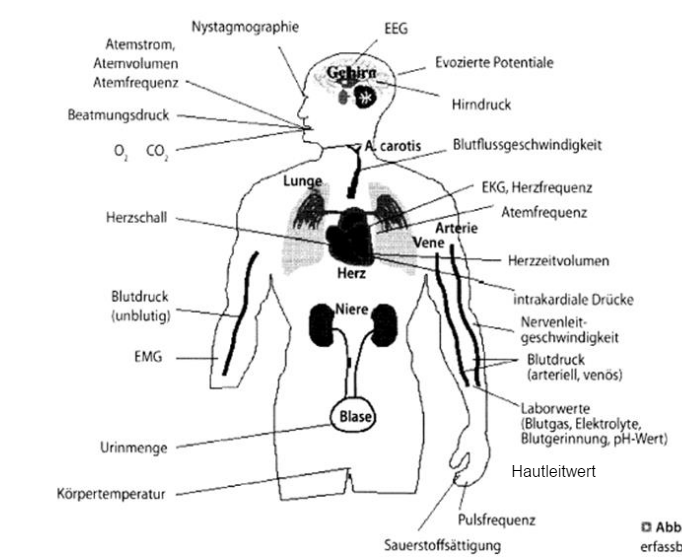
\includegraphics[scale=0.65]{Grafiken/beispielbiosig.png}

\subsection{Eigenschaften, Beschreibung, Darstellung}
Eigenschaften
\begin{itemize}
	\item Strukturgrößen: Länge, Fläche, menge, Volumen, Elastizität
	\item Funktionsgrößen: Temperatur, Druck, elektrische Potenziale, akustische Geräusche
	\item Beschreibung: Frequenz, Amplitude, Form, Auftrittszeitpunkt
	\item Darstellung: Zeit/Frequenzbereich, 2D oder 3D
	\item Auftreten: Stochastisch, stationär, periodisch, diskret
\end{itemize}

\subsection{Einteilung nach physikalischen Eigenschaften}
\begin{itemize}
	\item Bioakustische Signale: Herzschall, Lungengeräusche, Sprache
	\item Biochemische Signale: Stoffzusammensetzung, Konzentration
	\item Bioelektrische und biomagnetische Signale: Elektrische Potenziale, Ionenströme
	\item Biomechanische Signale: Größe, Form, Bewegung, Beschleunigung
	\item Biooptische Signale: Farbe, Lumineszenz
	\item Biothermische Signale: Körpertemperatur
\end{itemize}



\subsection{Messkette}
\begin{itemize}
	\item Applikation von Reizen, Strahlen, Substanzen, Wellen
	\item Primäres Messsignal Messen mit Fühler
	\item Signalverarbeiten (Linearisieren, Artefakterkennung, Rauschen entfernen)
	\item Biostatistik, Signalanalyse, Bildverarbeitung
	\item Bewertung
\end{itemize}


\subsection{Primäres Messsignal}
\begin{itemize}
	\item Medizin: Messsignal durch äußere Substanzen/Strahlen
	\item Biosignale: Invasiv, keine Anwendung äußerer Reize
	\item Meistens Signale, die vorhanden sind
	\item Primäres Messsignal: direkt vom Körper abgegriffen
\end{itemize}

\subsection{Reize}
\begin{itemize}
	\item Reize -> Reaktionen
	\item Mechanische, Elektrische, Akustische, Optische Reize, radioaktiv markierte Substanzen, Ultraschall, Röntgen, physische/psychische Reize
	\item Unwichtig für Benutzerschnittstellen, wichtig fürs Training
\end{itemize}

\subsection{Biosensoren}
\begin{itemize}
	\item Biosensoren erfassen Biosignale
	\item Mit Wandler verbunden oder ist direkt Wandler
	\item Wandler wandelt primär in sekundäres Messsignal um
	\item Sekundär Signal meist elektrisch
	\item Fühler ist eine biologische Detektionskomponente
\end{itemize}

\subsection{Biologische Detektionskomponente}
\begin{itemize}
	\item Sensitiv, spezifisch mit der Substanz
	\item Es können entstehen Wärme, Elektronen,Protonen, Lich, Gase, etc.
	\item Komponente besteht aus Enzymen, Mikroorganismen, Organellen, Zellverbände, Antikörper
\end{itemize}

\subsection{Anforderungen an Biosensoren}
\begin{itemize}
	\item Rückwirkungsfrei
	\item Reproduzierbar
	\item Konstantes Übertragungsverhalten
	\item Hohe Bioverträglichkeit
	\item Geringe Belastung
	\item Einfache Anwendung (Reinigung etc.)
	\item Entwicklungsziele für nächste Generation: Zuverlässiger, weniger Artefakte, Miniaturisierung, bessere Inkorporation, höhere Komplexität, Kanalanzahl, Berührungslosigkeit
\end{itemize}

\subsection{Wandler}
\begin{itemize}
	\item Wandeln primäres in sekundäres Messsignal
	\item Meist elektrisches Sekundärsignal
	\item Chemoelektrische Wandler, elektrische und magnetische Wandler, Mechanoelektrische Wandler, photoelektrische Wandler, thermoelektrische Wandler1
\end{itemize}

\subsection{Elektrische Wandler}
\begin{itemize}
	\item Ionenstrom->Elektronenstrom
	\item Ausdehnung (Dichte der Elektrodenplatzierung), Umgebungseinflüsse (Dreck, Tragekomfort) wichtig
	\item Größe: Mikro, Makroelektroden
	\item Platzierung: Oberflächen, Nadelelektroden
	\item Baufrom: Nadel, Schlaufe, Napf
	\item Materialien: Metallelektroden
\end{itemize}

\subsection{Mechanoelektrische Wandler}
\begin{itemize}
	\item Messung von Längenänderungen, Dehnungen, Druckschwankungen, Vibrationen, Blutfluss
	\item Besitzt Membran, die Kraftänderung detektiert (Auslenkung)
	\item Resistive Wandler: Membran = Spule, Längenveränderung des Dehnmessstreifens => Änderung des Widerstands
	\item Induktive Wandler: Membran = Spule, Verschiebung von Eisen/Ferritkern
	\item Kapazitive Wandler: Membran = Kondensator, Veränderung des Plattenabstandes => Kapazitätsänderung
	\item Kapazitive Wandler Beispiel: Kondensatormikrofon: Membran => Kondensator => Vibrationen verändern Entfernung der Platten => Kapazitätsänderung => Umwandlung in Spannungsschwankungen
	\item Piezoelektrische Wandler: Piezoelektrische Kristalle, mechanische Einflüsse in Richtung der polaren elektrischen Achsen bewirken Verformung => Verschiebung der Atome => Elektrische Ladung => Oberflächenladung
	\item Ladung ist Piezoelektrische Konstante $\times$ äußere Kraft
	\item Hall-Sonden: Nutzt Hall-Effekt: Strom durchflossen -> in orthogonales Magnetfeld => Spannung
	\item Photoelektrische Wandler: Erfassen Lichtabsorption und Lichtreflexion: Photowiderstand, Photodiode, Photoelement, Phototransistor: Lichtstärke => Stromänderung
	\item Thermoelektrische Wandler: Messung Atemstrom, Körpertemperatur
	\item Thermoelement: Temperaturdifferenz => Thermospannung
\end{itemize}

\subsection{Weitere Wandler - Indirekte Messung}
\begin{itemize}
	\item Biosignale oft indirekt erfasst
	\item Durch Einfluss von Strahlen, Wellen, radioaktive Stoffe
	\item PET, SPECT, MRT, CT; Angiographie
\end{itemize}

\subsection{Vorverarbeitung}
Elektrisches Sekundärsignal digitalisieren \\

\subsection{Vorverarbeitung - Differenzverstärker}
\begin{itemize}
	\item Zwei Eingänge, ein Ausgang
	\item $U_a = V*(U_e1-U_e2)$
	\item V Verstärkungsfaktor
	\item Wenn beide Eingänge gleich sind, Ausgangsspannung 0
	\item Brummen von Wechselstrom wird unterdrückt
	\item Linearität zwischen Eingangs und Ausgangssignal
	\item Verstärkung und Frequenzgang in Abhängigkeit des Biosignals
\end{itemize}

\subsection{Vorverarbeitung - Filterung}
\begin{itemize}
	\item Wirkt auf Frequenzkomponenten eines Signals
	\item Tiefpass- und Hochpassfilter
	\item Tiefpassfilter lässt tiefe Frequenzen passieren, dämpft hohe Frequenzen (EMG, EEG)
	\item Hochpassfilter lässt hohe Frequenzen passieren, dämpft langsame Wellen
\end{itemize}

Ideal: Linear, d.h. Änderung der Messgröße entspricht Änderung des Messwerts\\
Real nicht linear, da Außeneinwirkungen (Beispiel Messung Blutdruck, Gebilde zum Messen ist schwingungsfähig, daher leichte Änderungen)\\
Wesentliches Ziel ist Verbesserung der nicht-linearen Teile der Messkette

\subsection{Digitalisierung}
\begin{itemize}
	\item Sekundäres Messsignal ist kontinuierlich in Zeit und Amplitude
	\item Muss diskret im Computer sein
	\item Sampling und Quantisierung
	\item Quantisierung = Diskretisierung der y-Achse
	\item Sampling = Diskretisierung der x-Achse
\end{itemize}

\subsection{Digitale Signalverarbeitung}
\begin{itemize}
	\item Digitale Filterung
	\item Fensterung: Signal wird in Fenster unterteilt, um Zeitverlauf nachweisen zu können (Sprache, 16000 Samples/Sekunde -> 100 Fenster/Sekunde)
	\item Merkmalsextraktion (Wichtige Merkmale bezogen auf Kontext extrahieren)
	\item Kompression (Verringerung der Dimensionalität)
\end{itemize}

\subsection{Speicherung, Registrierung}
\begin{itemize}
	\item Direktschreibeverfahren: Ausgabe auf Registrierpapier
	\item Indirektschreibeverfahren: Photoschreiber und UV-Licht Schreiber
	\item Monitor: Analog oder Digitale Anzeige
	\item Speicherung auf Speichermedien
	\item Für Benutzerschnittstellen nur digitale Direktschreibung sinnvoll
\end{itemize}

\subsection{Übertragung}
\begin{itemize}
	\item Signale aus Körper
	\item Signale, die Auskunft geben über Person/implantierte Geräte
	\item Wired-Wireless, Bluetooth etc.
\end{itemize}

\subsection{Datenanalyse}
\begin{itemize}
	\item Messwerte: Zeitbereich/Frequenzbereich/Bildverarbeitung
	\item Beschreiben mit Systemen/Modellen/Simulationen
	\item Studien: Blindstudie (kein Placebo-Effekt), Doppelblindstudie (Untersucher kennt Faktoren nicht), Abhängige und unabhängige Stichproben, Langzeituntersuchungen
	\item Datenanalyse maschinell!
	\item Ablauf: Training + Klassifikation
\end{itemize}

\section{Erfassen von Biosignalen}


\subsection{Spracherkennung}
\begin{itemize}
	\item Traditionell: Mikrofon, Signal wird in elektrische Energie transformiert
	\item Probleme: Hörbarkeit (leise), Interferenz (Hintergrund), Privacy (öffentliche Orte)
	\item Alternativen?
\end{itemize}


\subsection{Stethoskop/NAM}
\begin{itemize}
	\item Kondensatormikrofon in Stethoskop
	\item "Hört" Körpervibrationen
	
\end{itemize}

\subsection{Bone-Conduction}
\begin{itemize}
	\item Resonanzkörper menschlicher Körper
\end{itemize}


\subsection{Geflüsterte Sprache}
\begin{itemize}
	\item keine/kleine Vibration der Stimmbänder
	\item gewisse Adaptionsschritte
	\item Throat microphone
	\item Close Talking microfone
\end{itemize}

\subsection{Bioelektrische Signale}
\begin{itemize}
	\item Potentialdifferenzen aus Nerven/Muskelvorgängen
	\item Elektroden leiten Signal ab
	\item Spannungsdifferenz benötigt
	\item Bipolare Ableitung: Potentialdifferenz zwischen zwei Elektroden auf elektrisch aktiven Gebieten
	\item Unipolare Ableitung/Referenzableitung: Eine Elektrode auf inaktivem Gebiet (Referenz)
\end{itemize}

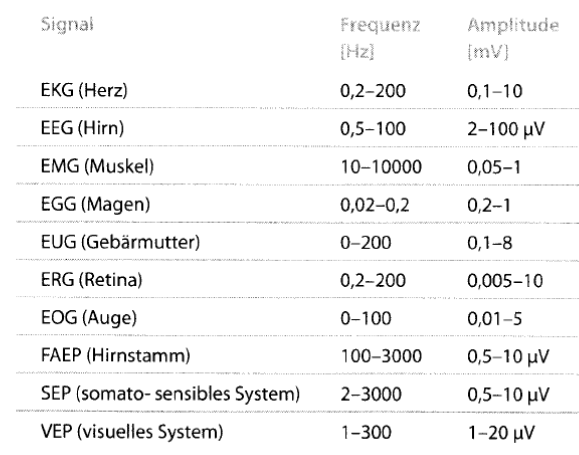
\includegraphics[scale=0.65]{Grafiken/bioelektrischesignalefreq.png}

\subsection{Erfassen elektrischer Felder}
\begin{itemize}
	\item Problem 1: Lokalisierung des elektrischen Feldes
	\item Anzahl Elektroden begrenzt
	\item Man geht bei EEG phänomenologisch vor, man erkennt Muster wieder, ohne alles zu verstehen
	\item Problem 2: Wandlung von Ionenstrom in Elektronenstrom
	\item Im Körper: elektr. Signalübertraung durch Ionenbewegungen
	\item Nötig, Ionen in Elektronenstrom zu wandeln, um erfassen zu können
	\item Elektroden erledigen dies
	\item Zwei Elektrodenarten:
	\item Redoxelektrode: Elektronen treten als Ladungsträger durch die Phasengrenze auf
	\item Ionen-Elektrode Ionen treten als Ladungsträger durch die Phasengrenze auf
\end{itemize}


\subsection{Nadelelektroden}
\begin{itemize}
	\item 2-6cm lang <1cm dick
	\item Verschiedene Seelen, Bipolare haben 2 Seelen
	\item Nadelelektronen unwichtig, da unkomfortabel (Einstich)
\end{itemize}


\subsection{Trockene/Feuchte Oberflächenelektroden}
\begin{itemize}
	\item Trockene: Direkter Körperkontakt, höherer Elektrode-haut Widerstand => Vorverstärker, groß, unhandlich
	\item Feuchte: Gel, meist verwendet
\end{itemize}

\subsection{Ionenelektrode}
\begin{itemize}
	\item Potenziale an Körperoberfläche gemessen
	\item Ankopplung mit Elektrolytpaste
	\item Metallischer Körper in Flüssigkeit => An Phasengrenze verschieben sich Ionen gegenseitig, Konzentrationen von Flüssigkeit/Metall ändern sich
	\item Ladungsverteilung
	\item Materialien haben chemische Potentiale
	\item => Ionenaustausch
	\item Gleichgewicht => Potentialdifferenz = Spannung (Galvani-Spannung)
	\item Stört Messung
	\item Messung über Referenzelektrode, da Bestimmung der Galvani-Spannung nicht möglich (Messung über Differenzen von zwei Galvani-Spannungen, zwischen bezugselektrode und untersuchende Elektrode)
	\item Durch Abnahme (Messen) von Strom, entsteht Stromfluss an Phasengrenze
	\item Dadurch Polarisation, Abweichung der Galvani Spannung
\end{itemize}

\subsection{Polarisation}
\begin{itemize}
	\item Thermodynamisches Gleichgewicht, kein Strom zuwischen Kathode und Anode
	\item Fließt durch Elektrode Strom, nicht Elektrodenpotenzial einen anderen Wert an
	\item Positiver(Anodischer) Strom = positive Abweichung
	\item Negativer (Kathodischer) Strom = Negative Abweichung
	\item Auslenkung der Elektrode heißt Polarisation oder Überspannung
	\item Durchtrittsüberspannung: Durchtritt durch Phasengrenze
	\item Diffusionsüberspannung: Ionentransport zur Phasengrenze
	\item Chemische Überspannung: Hemmung chemischer Reaktionen (Kristallisation)
	\item Polarisierbare Elektroden: Höher Überganswiderstand zwischen Körper und Elektrode, Verhalten wie Kondensator
	\item Bei Potenzialänderung erfolgt Stromfluss => Aufladung der Elektrode
	\item Unpolarisierbare Elektroden: Keine Hemmung des Ladungstransportes
	\item Ionenaustausch über Phasengrenze, Stromdichte S des Ladungstransports nur diffusionsbegrenz
	\item Reale Elektroden dazwischen (polarisierbar und unpolar.)
	\item Polarisierbare Metallelektrode: Positiv geladenene Metallionen in Elektrolytlösung: Osmostischer Druck und Feldkraft dagegen => elektrische Aufladung
	\item Aufbau einer entgegengesetzter Ladungsschickt im molekularen Abstand von der Phasengrenze
	\item Helmholtzsche Doppelschicht wie Kondensator => Polarisierbar
	\item Anwendungsbeispiel Ableitung höherfrequenter Signale
	\item Unpolarisierbare Metallelektrode: Metallelektrode wird mit Salz überzogen, Anion muss Bestandteil des Salzes sein
	\item Galvanispannungen kleiner und stabiler
	\item Geringere Überganswiderstände überall
	\item Ag/AgCl Elektroden für fast alle Signale einsetzbar
	\item Bei EEG wird Elektrolyt oder mit Kochsalzgetränktem Überzug verwendet
\end{itemize}

\subsection{Die Haut}
\begin{itemize}
	\item Wasserundurchlässig
	\item Leitfähigkeit durch Drüsen
	\item Kapazität umfasst Schichtaufbau der Haut
	\item Absenkung der Impedanz: Entfettung, Elektrodenpaste, Abtragen mit Sandpapier 
\end{itemize}

\subsection{Biokinetische Signale}
\begin{itemize}
	\item Messung von Bewegungen
	\item Direkte Erfassung EMG/EOG (Elektromyografie, Elektrookulografie)
	\item Indirekte Erfassung: Marker/Videoaufzeichnung
\end{itemize}


\subsection{Artefakte}
\begin{itemize}
	\item Störungen
	\item Ursachen Methoden, Proband, Speichertechnik (Kompression)
	\item Biologische Artefakte (vom Patienten)
	\item Technische Artefakte (Durch Geräte oder von außen)
	\item Biologische Artefakte (Augenbewegungen, Verspannungen, EKG Einstreuungen, Pulswellen, Schwitzen, Bewegungen)
	\item Technische Artefakte (Kontaktstellen, Kabeldefekte, Kabelbewegungen, fehlende Erdung, elektrostatische, magnetische oder elektromagnetische Wechselfelder
	\item Elektrische MEssmethode erzeugt viele dieser ARtefakte
\end{itemize}

\subsection{Artefaktbereinigung}
\begin{itemize}
	\item Testmethoedn anpassen (Abschirmen, möglichst viel konstant halten (Tageszeit, helligkeit)
	\item Technische Möglichkeiten: Bandsperrfilter, Hintergrundaktivitäten selektieren, Adaptive Filter, spezielle Algorithmen
	\item Manuelle/Automatische Artefaktrejektion
\end{itemize}

\section{Nervensystem, Informationsfluss im menschlichen Körper}

\subsection{Bausteine}
\begin{itemize}
	\item Neuronen: Transport und Verarbeitung von Signalen/Informationen
	\item Gliazellen: Hilfsapparat für Neuronen, Schutz, Versorgung, Stütze
\end{itemize}


\subsection{Neuronen}
\begin{itemize}
	\item Zellkörper(Soma): Verdickung, Verarbeitung von Informationen, wesentliche Stoffwechselvorgänge, enthält Zellkern
	\item Axon (Sender): Langer Zellfortsatz, transferiert Informationen vom Zellkörper zu anderen Zellen
	\item Dendriten (Empfänger): Zellfortsätze aus dem Zellkörper, sammeln Informationen von anderen Neuronen, stark bedornt, andere Neuronen können andocken
	\item Myelinscheide: umhüllt Axon, dient Beschleunigung der Leitungsgeschwindigkeit des Axons
	\item Vier Prinzipien der neuronalen Organisation:
	Grundlegende Strukturelle/funktionelle Einheit des Gehirns \\
	Axonenendigungen kommunizieren mit Dendriten anderer Neuronen nur an bestimmten Stellen, den Synapsen \\
	Verbindungsspezifität: Jede Nervenzelle kommuniziert nur mit ganz bestimmten anderen (spezielle Schaltkreise) \\
	Signalübertragung nur in eine Richtung
\end{itemize}

%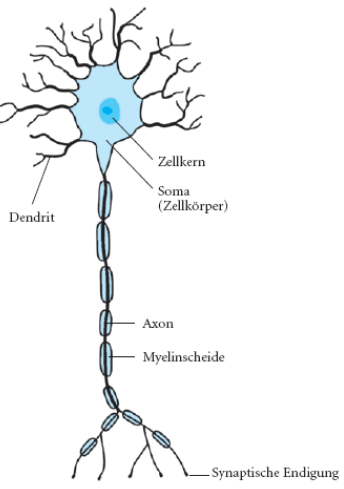
\includegraphics[scale=0.65]{Grafiken/neuron.png}


\subsection{Klassifikation}
\begin{itemize}
	\item Nach äußerer Gestalt (Pyramiden, Stern, ...)
	\item Nach Verbindungen:
	\item Sensorische Neurone: Informationsweitergabe über physikalische oder chemische Reize
	\item Motoneurone: Gehirn und Rückenmark, Steuern Aktivität von Muskel und Drüsenzellen
	\item Interneurone: Dienen als Umschaltstation zwischen sensorischen und motorischen
\end{itemize}


\subsection{Gliazellen}
\begin{itemize}
	\item "Führungselemente" beim Wachstum von Neuronen
	\item Stützelemente des Nervensystems
	\item Transportmedium 
	\item bilden Myelinscheiden
	\item Beeinflussung der Effektivität synaptischer Kontakte
	\item Wirken bei Blut/Hirn Schranke mit, schirmen Nervensystem von schädl. Stoffen im Blut ab
\end{itemize}

\subsection{Weiße/Graue Substanz}
\begin{itemize}
	\item Graue Substanz: Großhirnrinde (Cortex) und Kerne, besteht aus Neuronen Zellkörpern
	\item Weiße Substanz: Unterhalb des Cortex, bettet graue Substanz ein, besteht aus Nervenfasern
\end{itemize}


\subsection{Ruhepotential}
\begin{itemize}
	\item Ionenkonzentration im Zellinneren ungleich Zelläußeren => Potentialdifferenz
	\item = Membranpotential (Mensch -70mV Ruhepotential) (Zellinnere negativ außen)
	\item Zelle elektrisch polarisiert
	
\end{itemize}



\subsection{Messung}
\begin{itemize}
	\item Einstich in Zellinnere, zweite Elektrode außerhalb
\end{itemize}


\subsection{Permeabilitätsunterschiede}
\begin{itemize}
	\item Keine Ladungsausgleich da: Zellmembran nicht gleichermaßen durchlässig
	\item Ruhepotential aus unterschiedlcihen Verteilungen von Na, K, Cl, Proteinen
	\item Hoch permeabel: K+, Cl-
	\item Niedrig permeabel: Na+
	\item Undurchlässig: Proteinanionen
	\item Zellinnere K+, negative geladene Proteine
	\item Zelläußere: Na+, Cl-, Ca2+
	\item Elektrostatische Kräfte
	\item Thermische Bewegung-> Körperwärme
\end{itemize}

\subsection{Natrium-Kalium-Pumpe}
\begin{itemize}
	\item K+ in negativen zellinneren
	\item Cl- im positiven Äußeren
	\item Na+ außen (trotz Ladung)
	\item Natrium-Kalium-Pumpe befördert Na+ aus der Zelle ins Äußere (aktiver Transport)
	\item Membranproteine zwischen innen und außenseite (besitzen 3 Bindestellen für Na+ innen, 2 Bindungsstellen für K+ außen)
	\item K+ wandert durch Kaliumkanäle aus Zellinneren (passiver transport)
\end{itemize}

\subsection{Passiver Signaltransport}
\begin{itemize}
	\item Kein Energieverbrauch
	\item Potentialänderung
	\item Leitung schnell und verlustreich
	\item Nur bei kurzen Distanzen möglich (<1mm, z.B. Membranen der Dendriten)
	\item z.B. im Gehirn (informationsverarbeitung auf engem Raum)
\end{itemize}

\subsection{Aktionspotential (Spike)}
\begin{itemize}
	\item Zellen erzeugen Potenzialspitzen
	\item Verlustarme Weiterleitung
	\item Über lange Distanzen möglich
	
	\item Erregbare Nervenzellen reagieren uaf Reiz (Ionenleitfähigkeit der Membran ändert sich)
	\item Können weitaus höhere Spannung als der ursprüngliche Reiz verursachen
	\item Spannungsänderung durch Reiz => von Innen nach außen gerichteter Strom durch Membran
	\item 3 Phasen
	\item Depolarisation: schnell: Ionentör öffnet sich, Natriumeinstrom: Potential wird größer
	\item Repolarisation: langsam: Kaliumtore öffnen sich, Kaliumausström: Potential fällt ab
	\item Nachhyperpolarisation: Kaliumtore schließen sich nur langsam: Potential fällt unter Ruhepotential
	\item Nach Aktionspotential: Membran schwer/überhaupt nicht erregbar, Refraktärphase
	
\end{itemize}

\subsection{Saltatorische Erregungsleitung}
\begin{itemize}
	\item Ausbreitung des Aktionspotential entlang des Axons ist sprunghaft
	\item Myelinscheiden wie Isolatoren
	\item An Ranvier-Schnürringen sind unmyelinisierte Stellen (Hohe Konzentration an sspannunggesteuerten Na-Kanälen, Aktionspotential wird wieder aufgefrischt)
	
\end{itemize}

\subsection{Aktionspotentiale Eigenschaften}
\begin{itemize}
	\item Alles- oder Nichts: Stärke des Reizes keien Auswirkung auf Höhe AP
	\item Stärke des Reizes bestimmt Geschwindigkeit des AP, (Länge Refraktärzeit)
	\item Reizstärke in Frequenz der AP umkodiert
\end{itemize}

\subsection{Informationsübertragung: Synapse}
\begin{itemize}
	\item Signalübertragung durch Synapsen
	\item Definition Synapse: Verbindungsstelle zwischen zwei Neuronen oder einem Neuron und einer Zelle des Erfolgsorgans (z.B. Muskelzelle) an der Information weitergegeben wird
	\item Axon - Dendrit oder Axon - Soma
	\item Elektrische Synapse
	\item Chemische Synapse
\end{itemize}

\subsection{Elektrische Synapse}
\begin{itemize}
	\item Nahe Zellmembranen
	\item Röhrenartige Verbindung
	\item Schnell
	\item Informationsübertragung in beide Richtungen
	\item Synchronisation von Zellverbänden mit identischen Funktionen: Muskelzellen des Herzens, Muskelzellen der inneren Organe, Neuronenverbände im Gehirn
\end{itemize}

\subsection{Chemische Synapsen}
\begin{itemize}
	\item Spalt größer als bei elektrische Synapse
	\item Spalt wird mit chemischen Botenstoffen überbrückt
	\item Ausganszelle sendet Botenstoff, löst Prozess an Membran von Empfängerzelle aus -> Ionenwanderung
	\item Asymmetrisch
	\item Nicht so schnell
	\item Zentralnervensystem Informationsverarbeitung
	\item Präsynaptische Endigung (Sender)
	\item Postsynaptischer Membranbereich (Empfänger)
	\item Ablauf Informationsübertragung:
	\item Membranerregung in präsynaptische Endigung
	\item Neurotransmitter in synaptischen Spalt
	\item Verteilt sich darin
	\item Erreich Empfängermoleküle (Rezeptoren) an postsynaptischer Membran
	\item Transmitterstoffe wirken an Repezeptoren
	\item Ionenkanäle öffnen sich -> Potentialveränderung -> evtl. neues AP
	\item Chemische Übertragung: schnell, gezielt, kurz
	\item Neurotransmitter ist in den Vesikeln der präsynaptischen Endigung gespeichert
	\item Zellsignal -> Vesikel verschmelzen mit Zellmembran -> Gießen Transmitter in Spalt
\end{itemize}

\subsection{Potenzialveränderungen}
\begin{itemize}
	\item Je nach verschobener Ionensorte
	\item Depolarisation (Inneres wird positiver): Exzitatorisches postsynaptisches Potenzial (EPSP)
	\item Hyperpolarisation (Zellinneres wird negativer): Inhibitorisches postsynaptisches Potenzial (IPSP)
	\item Alles oder nichts für AP
	\item Membranbereich muss erregbar sein
	\item Nicht alle Potenzialverschiebungen der postsynaptischen Membran geben AP
	\item Neurotransmitter dockt nur kurz, nach Reaktion Abtransport
\end{itemize}


\subsection{Drei Zustände der postsynaptischen Membran}
\begin{itemize}
	\item Hyperpolarisierung, Ruhepotenzial noch weiter zu negativeM Wert verschoben = IPSP
	\item Depolarisierung, Ruhepotenzial wird weniger negativ oder positiv (EPSP), kein AP
	\item Zielzelle soweit depolarisiert, dass AP auftritt -> Erregungsübertragung von Ausgangs- zu Zielzelle
\end{itemize}

\subsection{Verrechnung zum Gesamtergebnis}
\begin{itemize}
	\item Axonhügel kodiert Höhe des Membranpotenzials in Impulsfrequenz der axonal auslaufenden Aktionspotenziale
	\item Mechanismen zum Verrechnen
	\item Räumliche Summation, Verstärkung von mehreren Potenzialen, die in zeitlich geringer Versetzung einlaufen
	\item Zeitliche Summation: Schnelle Aufeinanderfolge einlaufender Impulse zustande, Transmitterausschüttung kann sich erhöhen
	\item Präsynaptische Hemmung: Synapse von hemmendem Neuron kann Transmitterausschüttung verringern
\end{itemize}

\subsection{Zusammenfassung Informationsweiterleitung}
\begin{itemize}
	\item Aktionspotenzial kommt an präsynaptischer Endigung an
	\item => Öffnung spannungsgesteuerter Kalziumkanäle
	\item Einstrom Kalzium verursacht Verschmelzen der transmittergefüllten Vesikel mit der Membran
	\item Transmitter läuft in den synaptischen Spalt
	\item Transmitter dockt an spezifische Rezeptoren der postsynaptischen Endigung an
	\item Wird an der Membran ein Schwellwert überschritten, öffnen sich spannungsgesteuerte Natriumkanäle
	\item Lawinenartiger Natriumeinstrom löst ein Aktionspotenzial aus
	\item Kann weitergeleitet werden->Repeat
\end{itemize}
Ein Aktionspotenzial wandert nicht, es induziert neue AP in benachbarter Membranregion

\subsection{Anatomie Nervensystem}
\begin{itemize}
	\item Topographie: zentrales nervensystem: Gehirn, Rückenmark
	\item Peripheres Nervensystem: Spinalnerven, Hirnnerven, Körpernerven
	\item Funktionelle Gliederung:
	\item Somatisches Nervensystem: Sinnesorgane, Skelettmuskulatur
	\item Autonomes/Vegetatives: Innere Organe, Glatte Muskulatur
\end{itemize}

\subsection{Zentrales nervensystem}
\begin{itemize}
	\item Rückenmark und Gehirn
	\item Verarbeitung afferenter Signale (von Peripherie zum Gehirn)
	\item Senden efferenter Signale (von Gehirn zu peripherie)
	\item Denken, Lernen, Sprache, Gedächtnis, etc.
	\item Kontrolle Atmung, Herz, etc.
	\item Rückenmark: Spinale Reflexe (monosynaptisch, polysynaptische Reflexe)
	\item Gehirn: Verschiedene Teile des Hirns verantwortlich für verschiedene Teile der Körperfunktionen, 2 Hemisphären (links, rechts), Cerebral cortex äußerster Teil des Großhirns, gefaltet um Oberfläche zu erhöhen
	\item Zwischenhirn: Weiterleitung sensorischer Informationen
	\item Komplexe kognitive Prozesse: Aktivität in verschiedenen Arealen
\end{itemize}

Gehirnteile zuständig für Körperteile
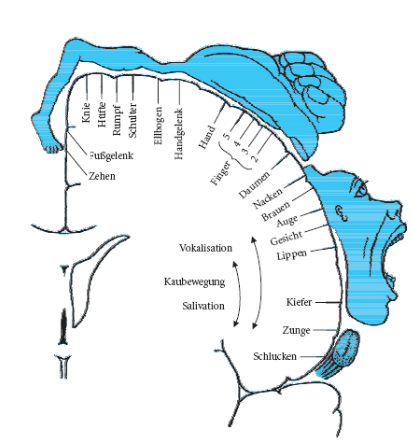
\includegraphics[scale=0.65]{Grafiken/homunkulus.png}

\subsection{Neuronale Organisation des Kortex}
\begin{itemize}
	\item Drei Neuronentypen: Pyramidenzellen, Sternzellen, Spindelzellen
	\item Übereinander geschichtete Zellen haben oft ähnliche Aufgaben (kortikale Säulen)
	\item Feinstrukturen erkennbar
\end{itemize}

\subsection{Autonomes Nervensystem}
\begin{itemize}
	\item Weitgehend unbewusst
	\item Herz, Lunge, MagenDarm, Gefäße und Drüsen
	\item Elementar für Körper
\end{itemize}

\section{Digitale Signalverarbeitung}
\subsection{Digitalisieren}
\begin{itemize}
	\item Zeit und Amplitude von kontinuierlich -> diskret
	\item Sampling: Diskretisierung der Zeit
	\item Quantisierung: Diskretisierung der Amplitude
\end{itemize}

\subsection{Quantisierung}
\begin{itemize}
	\item y-Achse in gleichlange Intervalle aufteilen
	\item $q[i]$ kann nur Werte haben, die den Zentren der Intervalle entsprechen
	\item Funktion nimmt Mittelwert des Intervalls an, in der sie sich grade befindet
	\item Quantisierungsfehler $e[i] = f[i] - q[i]$
	\item Durchschnittlicher Quantisierungsfehler ist $f_max-f_min/2n$ (Funktion zuwischen fmax fmin und n Intervalle auf y-Achse)
	\item Signal-Noise Ratio = $E\{f^2[i]\} / E\{e^2[i]\}$
\end{itemize}


\subsection{Signal-Rausch-Verhältnis}
\begin{itemize}
	\item Störung e (Artefakte, Messungenauigkeit, Quantisierung)
	\item Verhältnis zwischen Energie des Signals und Energie des "Rauschens"
	\item Messung in Dezibel, da Rauschenergie << Signalenergie
\end{itemize}


\subsection{Sampling/Abtastung}
\begin{itemize}
	\item Input: Analoge Signal in Zeitbereich x(t)
	\item Output: Digitale Repräsentation 
	\item Abtastrate sehr wichtig (da sinuskurven, eventuell falsche Annahmen)
	\item Informationsverlust
	\item Abtastrate in Hertz
	\item Undersampling
	\item Aliasing (Falsche Annahmen führen zu falschem Kurvenverlauf
	\item Hohe Abtastrate: relativ sicher
	\item Niedrige Abtastrate: Falsche Frequenz gefunden
\end{itemize}

\subsection{Nyquist-Theorem}
\begin{itemize}
	\item Signale bandbegrenz: maximale Frequenz
	\item Theorem von Nyquist: $f_l$-bandbegrenztes Signal wird mit Frequenz $>2fl$ abgetastet => original Signal aus den Samples vollständig rekonstruierbar
	\item Ansonsten Aliasing
	\item $2f_l$ Nyquist-Rate
	\item maximal korrekte Frequenz $f_l$ Nyquist-Frequenz
\end{itemize}

\subsection{Frequenzanalyse}
\begin{itemize}
	\item Continuous-time Fourier transform (CTFT)
	\item Discrete-Time Fourier transform (DTFT)
	\item Short-time Fourier transform (STFT) (benötigt Fensterung)
	\item Frequenz "SChwingungen pro Zeiteinheit, 1Hz=1Schwingung/Sekunde"
	\item Bisher nur darstellung Zeit->Amplitude
	\item Neue Darstellung zeit->Vorkommen einer Frequenz
	\item $\rightarrow$ Kurve darstellbar als Überlagerungen von vielen Frequenzen
	\item Warum Signal im Frequenzbereich darstellen?
	\item Nützlich für Signalverarbeitung, leichtes Verständnis des Signals, Filter gut beschreibbar
	\item Frequenzrepräsentation eines Signals = Spektrum
\end{itemize}

\subsection{Continous-Time Fourier Transform CTFT}
\begin{itemize}
	\item Fourier Transformierte:
	\item $X(\omega) = F(x)(\omega)= \int_{-\infty}^\infty x(t)e^{-j\omega t}dt $
	\item Wichtigste Eigenschaften:
	\item Linearität: $F((x+y)(t)) = F(x(t)) + F(y(t))$ und $F(a\times x(t)) = aF(x(t))$
	\item Umkehrbarkeit: Auf geeigneten Definitionsbereichen gibt es ein Inverses = KEIN INFORMATIONSVERLUST
	\item $X(\omega)$ ist ein Wert, der angibt, welchen "Anteil" die Frequent $\omega$ am Eingabesignal hat
	\item Fourier-Transformierte im allgemeinen komplex, Betrag $|X(\omega)$ ist die zur Frequenz gehörende Amplitude Winkel zwischen real und imaginär Teil ist Phase
	\item Problem: Fourier transformation gibt keine Informationen, wann ein Frequenzanteil aufgetreten ist
\end{itemize}

\subsection{Discrete-Time Fourier Transform (DTFT)}
\begin{itemize}
	\item Ersetze in der Formel vorher kontinuierliches x(t) mit diskreten Signal $x[n]$
	\item Wenn $x[n]$ durch diskretes Sampling einer kontinuierlichen Funktion entstanden ist, approximiert die DTFT die kontinuierliche Fourier-Transformation.
	\item Die DTFT ist periodisch in $\omega$ mit Periode $2\pi$, daher betrachtet man im Frequenzbereich nur die Frequenzen von $-\pi$ bis $\pi$
	\item In der DTFT sind nur Frequenzen unterhalb der halben Abtastrate (nyquist-Frequenz) korrekt wiedergegeben. $\pi$ entspricht dann der maximalen Frequenz.
	\item Scheller Algorithmus (FFT) um diskrete Fourier-Transformation auszurechnen => gute Praxisanwendbar
	\item DTFT komplex
	\item Selbes problem wie bei CTFT, keine Infromation über Zeit, wann bestimmte Frequenz aufgetreten ist	
\end{itemize}

Wenn wir DTFT eines diskreten Signals ausrechnen, sind Frequenzen auf den Bereich $[-\pi,\pi]$ normiert.\\
Frequenzen im diskreten Signal hängen von Abtastrate ab.\\
Maximale Frequenz $\pi$ im diskreten Signal $\Leftrightarrow$ Nyquist Frequenz im kontinuierlichen Signal \\
Realfall: Betrag wichtig, Phase ignoriert, Abtastrate = Nyxquist-Rate, Fensterlänge

\subsection{Praxis}
\begin{itemize}
	\item Ergebnis aus FFT so lang wie Fenster
	\item Negative und positive Frequenzen, nur Hälfte interessant, Fensterlänge/2 = Anzahl Frequenzbins
	\item Nyxquist-Frequenz / Frequenzbins entspricht Bin-Breite
	\item Fenstergröße kritisch, Tradeoff zwischen zeitlicher und Frequenzauflösung
	\item Also: Sampling-Rate 80KHz
	\item Nyquist-Frequenz: 40KHz
	\item 20ms Fenster = 0.02*80000= 1600 Sample -> 800 Frequenzbins
	\item Bin-Breite = 40000/800 = 50Hz
\end{itemize}

\subsection{Fensterung}
\begin{itemize}
	\item Problem Fourier-Transformation: Signal ändert sich mit der Zeit, aber keine Informationen in Fourier-Transformation enthalten, wann welche Frequenzanteile vorgekommen sind
	\item Lösung: Zerlegen in kleine Abschnitte, Fensterung/Framing
	\item Vorgehensweise:
	\item Multipliziere Signal abschnittsweise mit Fensterfunktion
	\item Erhalte für jedes Fenster ein Resultat
	\item Funktion der Zeit
	\item Fenster/Frames sollten überlappen => weniger Ungenauigkeiten
\end{itemize}

\subsection{Short time Fourier transform STFT}
\begin{itemize}
	\item Fensterung + Anwendung der DTFT auf jedem Fenster
	\item Fensterlänge und verschiebung bestimmen Auflösung (In der Spracherkennung, Fensterlänge 16ms, Verschiebung 10ms)
	\item Frequenzanteil in 16ms Schritten
	\item Neues Problem Fensterung verzerrt das Spektrum
	\item STFT grundlegend für viele Signalverarbeitungen
	\item Fensterung ermöglicht andere nützliche Informationen
	\item Frame-base power (Energie im Fenster)
	\item Frame-based mean (Mittelwert im Fenster)
	\item STFT erzeugt aus Ursprungssignal eine Folge von Tokens im Zeitbereich
	\item Tokens sind Vektoren die Frequenzanteile des Frames enthalten
	\item Tokens können weiterverarbeitet werden
	\item Mit anderen Frame-basierte Vorverarbeitungen verfährt man entsprechend
\end{itemize}

\subsection{Fensterfunktion}
\begin{itemize}
	\item Wie sollte Fensterfunktion gewählt werden?
	\item Frequenzspektrum des Signals wenigstmöglich verändern
	\item Fensterung erfolgt durch Multiplikation im Zeitbereich, was einer Faltung im Frequenzbereich entspricht
	\item d.h. das Spektrum wird mit der fourier-transformierten Fensterfunktion gefaltet
	\item Dirac-Impuls: Neutrales Element für Faltungsoperation
	\item Da die Fensterung im Frequenzbereich einer Faltung entspricht, hätten wir gern ein Fenster, das "so gut wie möglich" gleich dem Dirac-Impuls ist (im Frequenzbereich)
\end{itemize}
Rechte Funktion sollte möglichst gut Dirac-Impuls (für n = 0: 1, sonst 0) sein
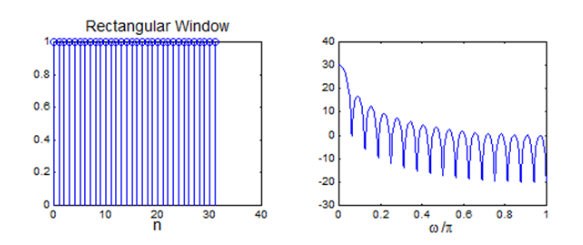
\includegraphics[scale=0.65]{Grafiken/rechteckfensterfunktion.png}\\
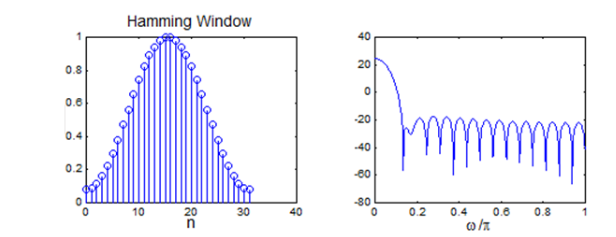
\includegraphics[scale=0.65]{Grafiken/hammingfenster.png}\\
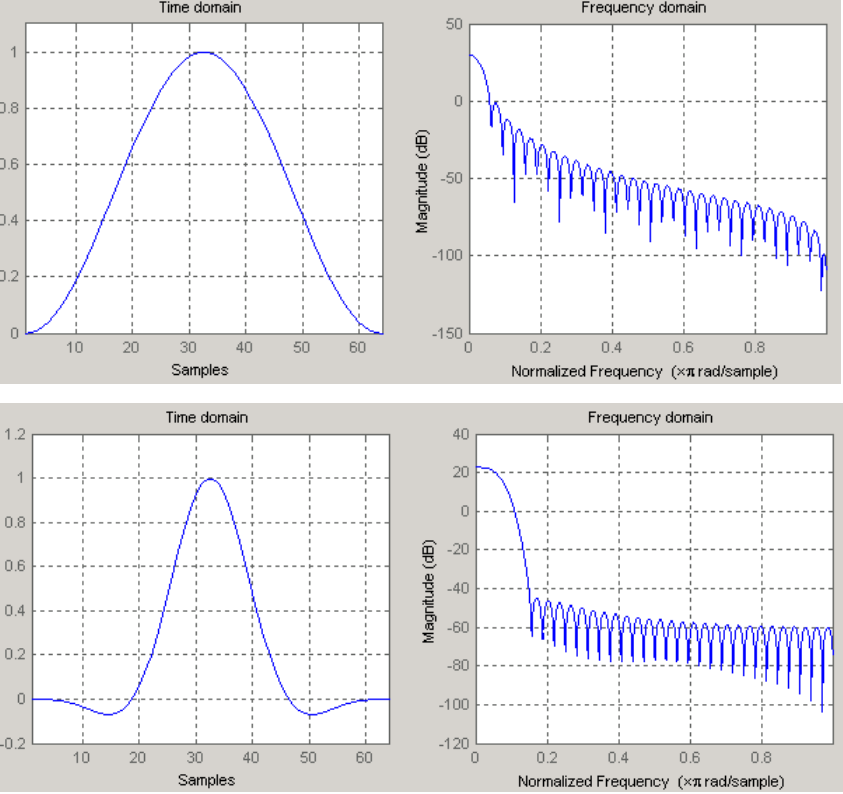
\includegraphics[scale=0.65]{Grafiken/hanningflattopfenster.png}

Quadratisches Mittel in Fenster in EMG benutzt als Feature für Muskelaktivität\\
Andere Features in Fenstern: \\
Standard Statistik Werte (Mittelwert, Varianz, Wölbung, Schiefe)

\subsection{Spektrogramm}
\begin{itemize}
	\item Frequenzanteile einer Funktion über Zeit: Spektrogramm
	\item x-Achse Zeit
	\item y-Achse: Frequenz
	\item Abhängige Variable: Frequenzanteil zum betreffenden Zeitpunkt, je roter, desto höher
	\item Fensterlänge haben wichtigen Effekt
	\item Kurze Fenster: ungenau im Frequenzbereich
	\item Lange Fenster: ungenau im Zeitbereich
	\item Kompromiss: Fenstergröße empirisch finden, Genauigkeit begrenzt (Heisenbergsche Unschärferelation)
	\item Filter "verhscmieren und verzerren" Signal auf der Vertikalten Achse, kann unwichtige Fluktuation unterdrücken, Erkennungsleistung wird typischerweise verbessert
\end{itemize}

\section{Filter}
Filter wirken auf Frequenzen des Eingabesignals.\\
Wichtige Signalverarbeitungsschritte (Rauschunterdrücken, etc) durch Filter repräsentieren.\\
Impulsantwort und Frequenzantwort (Übertragungsfunktion) eines Filters charakteristisch

\subsection{Lineares zeitinvariantes Filter}
\begin{itemize}
	\item H Filter, der Eingabesignal $x[n]$ in Ausgabesignal $y[n]$ transformiert
	\item Annahme: Transformation ist linear, zeitinvariant, kausal, endliches Eingabesignal nur endliche Ausgabe
	\item Impulsantwort: Ausgabe zu einzelnem Impuls (Dirac Impuls $\delta$)
	\item x ist eine gewichtete Summe von verschobenen Impulsen!
	\item $x[n] = \sum x[v] * \delta[n-v]$
	\item h Impulsantwort (aus Filter? nicht sicher)
	\item Ausgabe $y[n] = \sum x[v] * h[n-v]$
	\item Diese Operation ($:= x*h$) ist Faltung, Ausgabesignal $y = x*h$
	\item Wenn Signale in Frequenzbereich transformiert werden, wird die Faltung zu einfacher Multiplikation (immer noch linear)
	\item Lineare, Zeitinvariante Filter sind Multiplikationen im Frequenzbereich
	\item Jeder Frequenzanteil (komplex) wird mit einem (komplexen) Faktor multipliziert -> verstärken/abschwächen bestimmter Frequenzen
	\item Zusätzlich Phasenverschiebungen
	\item $y[n] = (h*x)(n)$ ist im Frequenzbereich dasselbe wie $Y(e^{j\omega}) = H(e^{j\omega}) * X(e^{j\omega})$
	\item H() Übertragungsfunktion
	\item Wenn Eingabe reine Frequenz: $H(e^{j\omega})$ Frequenzgang
	\item $|H(e^{j\omega})|$ ist Amplitudengang
	\item Imaginärteil ist Phasengang
\end{itemize}


\subsection{Bandpassfilter}
\begin{itemize}
	\item Hoch, Tiefpassfilter lassen hohe/tiefe Frequenzen durch
	\item Bandpassfilter: lassen bestimmte Frequenzen durch
	\item Bandsperrfilter: Sperren bestimmte Frequenzen
	\item Filter, multiplizieren im Spektralbereich = Flatungsoperation im Zeitbereich
	\item (Hilber-Transformation erzeugt Phasenverschiebung)
	\item (Differentiator approximiet ableitung)
\end{itemize}

Digitale Filter: Beispiele
\begin{itemize}
	\item Wir betrachten nur lineare, zeitinvariante Filter (LTI - linear time invariant)
	\item (Finite impulse response) Nichtrekursive Filter: Wenn das Eingabesignal endlich ist, ist Ausgabe auch endliuch
	\item (Infinite impulse response) Rekursive Filter: Endliche Eingabe KANN unendliche Ausgabe erzeugen (die aber in Realität gegen 0 läuft)
	\item Beispiel: $y[n] = x[n] - 0.5 x[n-1] + 0.2y[n-1]$
	\item Beide können im Frequenzbereich betrachtet werden
\end{itemize}

\subsection{z-Transformation}
\begin{itemize}
	\item Generalisierung der diskreten Fourier Transformation
	\item Ziel: Eigenschaften von Filtern besser beschreiben
	\item DTFT: $X(\omega) = \sum x[n]e^{-j\omega nt_a}$
	\item Z-Transformation: $X(z) = Z(x[n]) = \sum x[n] z^-n$
	\item Z komplex
	\item DTFT: nur $|z| = 1$
	\item Z-Transformation: z alle komplexen Werte
	\item DTFT ist die Einschränkung der z-Transformation auf den Einheitskreis
	\item z-Transformation linear
	\item Die z-Transformation konvergiert nicht immer und nicht überall, aber bei allen Folgen mit endlicher Energie enthält der Konvergenzbereich den Einheitskreis der z-Ebene
	\item z-Transformation überführt Faltung im Zeitbereich in Multiplikation im z-Bereich
	\item Verschiebungseigenschaft: Wenn $x[n] = X(z)$ (nicht gleich, gleichbedeutend)
	\item Dann $x[n-N] = z^{-N}X(z)$
	\item Interessant für Filter
\end{itemize}

\subsection{Filter als Differenzengleichung}
\begin{itemize}
	\item Filter H, möglicherweise rekursiv
	\item Im Zeitbereich: Differenzengleichung: $y[n] = -a_1y[n-1] - a_2y[n-2] ...a_my[n-m] + b_0x[n] + b_1x[n-1] ... + b_lx[n-l]$
	\item Umformen: Nur y auf der einen Seite, x auf der anderen
	\item Transformieren: Summe von y $=(a*y)[n] = A(z) * Y(z)$
	\item Summe von x $=(b*x)[n] = B(z) * X(z)$ 
	\item rechte Seite jeweils in Spektralbereich
	\item a und b Vektoren, $a_0$ normiert auf 1
	\item Definition Übertragunsfunktion im z-bereich
	\item $H(z) = \frac{Y(z)}{X(z)} = \frac{B(z)}{A(z)}$
	\item $Y(z) = H(z) * X(z)$
	\item (Wenn Folge von y[n], y[n-1] ist a genau Koeffizientenfolge, analog x[n]
	\item Nullstellen von Zähler von H und Nullstellen von Nenner geben Nullstellen und Pole (Unendlichkeitsstellen) an
	\item z(z-1) im Zähler => Nullstelle z=1
	\item z(z-1) im Nenner => Polstelle z=1
	\item Nullstellen und Pole => Eigenschaften des Systems
	\item Resonanzfrequenz: Polstelle auf Einheitskreis (theoretisch) niemals abklingbar
	\item FIR (Nichtrekursive) Filter haben KEINE POLSTELLEN außer Ursprung, daher endlcihe Impulsantwort
\end{itemize}

\subsection{Von z-Transformation auf DTFT}
\begin{itemize}
	\item Betragt der DTFT=z-Transformation auf dem Einheitskreis
	\item Jeder Punkt auf Einheitskreis: Betrag der DTFT = Produkt der Distanzen zu den Nullstellen, dividiert durch Produkt der Distanzen zu Polstellen der z-Transformation
	\item Damit Auswirkungen eines Filters auf Frequenzen beschreiben
	\item Dafür gesamte z-Ebene betrachten, nicht nur Einheitskreis
\end{itemize}


\subsection{Filterdesign}
\begin{itemize}
	\item Wie bestimmt man Filterkoeffizienten?
	\item Beschreibe Eigenschaften im Frequenzbereich
	\item Bestimmte Übertragungsfunktion H
	\item Transformiere H zurück in Zeitbereich, erhalte Filterkoeffizienten (Impulsantwort)
	\item Problem: endlcihe Arithmetik geben keine idealen Filter
	\item exakter Bandpassfilter hat unendlich lange Impulsantwort
	\item Man muss Abstriche machen
\end{itemize}

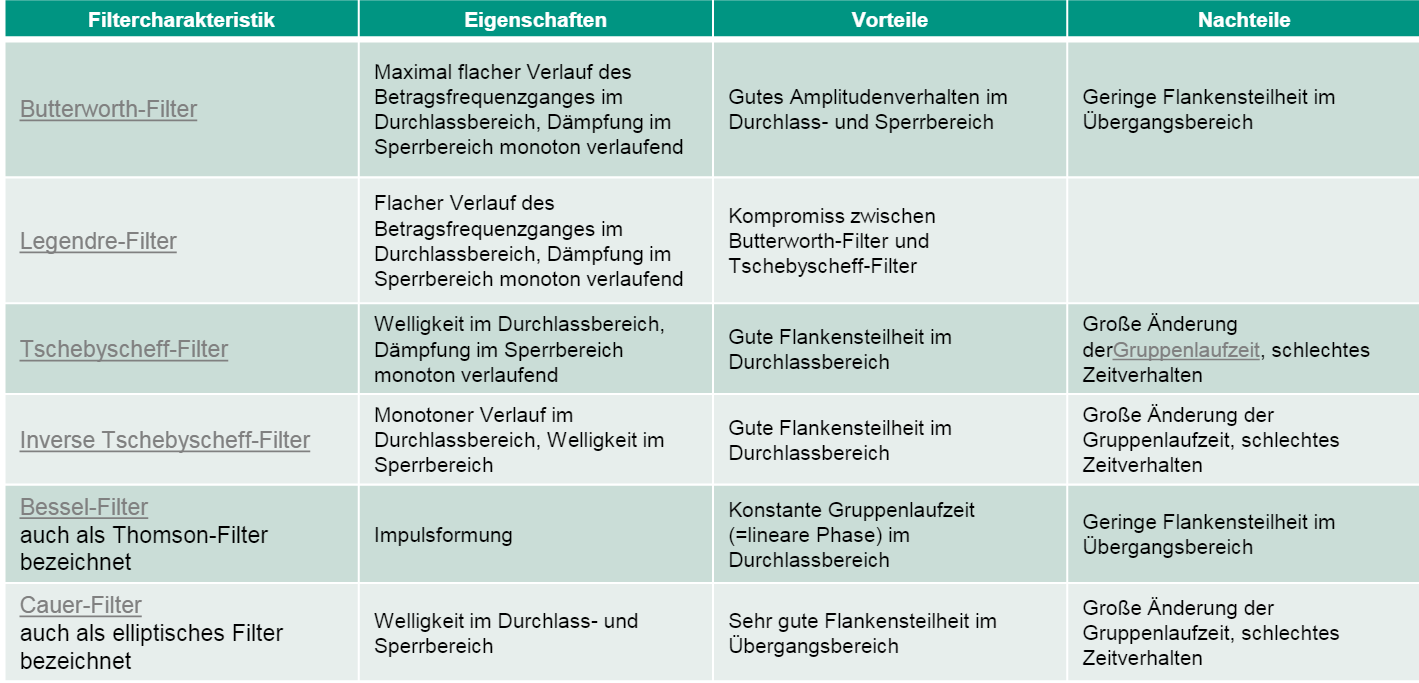
\includegraphics[scale=0.65]{Grafiken/tabelle.png}

Typischer Fehler bei Filtern, wenn Signal mittelwertverschoben braucht Filter lange um einzuschwingen (40sekunden im beispiel)

\subsection{Kompression}
\begin{itemize}
	\item Hochdimensionales Signal
	\item Redundante Informationen
	\item Signal und rauschtrennung
	\item Rechenzeit, speicherplatz reduzieren
	\item hochdimensionales System generell schlecht
\end{itemize}


\subsection{Fluch der Dimensionalität}
\begin{itemize}
	\item Pro Dimension exponentiell mehr Trainingsdaten für guten Klassifikator (10cm -> 100 quadratcm)
	\item Jede Dimension muss viele Informationen liefern um Aufwand zu rechtfertigen
\end{itemize}

Kompression: Verringerung der Dimensionalität der Daten, bedeutungstragende Merkmale belassen
\begin{itemize}
	\item Gegeben: Menge von Feature Vektoren, die Ausschnitte des Signals repräsentieren
	\item Selektionsmethode Feature-Auswahl: 20 Feature-Komponenten, nehmen beste 10
	\item Kompressionsmethoden: Sprachsignal Filterbänke, nichtparametrisch, unüberwacht: PCA, ICA, überwacht: LDA
\end{itemize}

\subsection{Feature Selection}
\begin{itemize}
	\item Theoretisch alle Dimensionen durchgehen -> unpraktikabel
	\item Feature Ranking: Qualitätsmaß für jede Dimension berechnen
	\item Threshold für Qualitätsmaß, behalte beste Dimensionen
	\item DEVELOPMENT SET! NICHT TESTSET BENUTZEN
	\item Subset selection
	\item Evaluiere Untermenge von Features und vergleiche sie
	\item Forward Feature Selection: Zunahme von bester Dimesion Schritt für Schritt
	\item Backwards Feature Selection: Nehme alle und schreiche unwichtige nacheinander heraus
\end{itemize}


Korrelationen: Zusammenhang zwischen mehreren Variablen, Kovarianz der beiden Variablen geteilt durch produkt Standardabweichungen \\
Korrelation heißt nicht Kausalität \\
Je höher Dimension, desto warscheinlicher falsche Korrelation\\
Man korreliert zwei Labens und Merkmale\\
Funktioniert nur für 2 Klassen Probleme\\
r Quadrat = Coefficient of detemination, schätzt Anteil der Varianz in Y der durch X erklärt werden kann \\
Unechte Korrelationen durch Zufall, ungesehene Faktoren


\subsection{Fisher ratio}
\begin{itemize}
	\item Maß für discrimative Kraft einer Variable
	\item Fishers ratio = $\frac{(m_1-m_2)^2}{v_1+v_2}$
	\item m Mittelwert, v Varianz
	\item oft als Pre selektions Kriterium für Merkmale verwendet
	\item schneller berechenbar als komplexere Kriteren (mutual Information)
\end{itemize}

\subsection{Mutual Information}
\begin{itemize}
	\item Korrelationen nicht berechenbar
	\item Besser Mutual Information: Informationen in X und Y gleich
	\item Um wieviel wird die Unsicherheit der einen Variable reduziert, wenn man die andere kennt
	\item Diskrete Variable $I(X;Y) = \sum_{y\in Y} \sum_{x\in X} p(x,y) \log(\frac{p(x,y)}{p(x)p(y)})$
	\item Kontinuierliche Variable $I(X;Y) = \int_Y\int_Xp(x,y)\log(\frac{p(x,y)}{p(x)p(y)})dx dy$
\end{itemize}

\subsection{Maximum Relevance Minimum Redundancy}
Nur Qualitätsmaß nicht ugt, da Merkmale mit niedriger Qualitätsindex manchmal wichtige Informationen enthalten\\
Idee: Gewichtete Relevanz und Redundanz (unter Merkmalen)\\
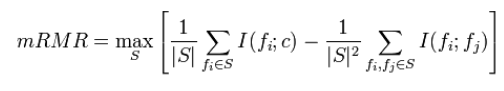
\includegraphics[scale=0.65]{Grafiken/mrmr.png}

\subsection{Wrapper}
Prädiktives Modell um Feature Subsets zu bewerten\\
Trainieren von Model, das auf hold-out Set getestet wird\\
Computational sehr teuer\\
Vorgehen:\\
Klassifiziere hold-out Set mit jedem einzelnen der m Features\\
Wähle Feature mit bester Klassifikationsleistung\\
Klassifizieren hold-out Set mit dem selektierten Feature und jedem anderen Feature, wähle beste Kombination\\
Weitermachen mit zweiter-Kombination und jedem anderen Feature?
\\ \\
Probleme: Einfache Algorithmen, eventuell nicht anwendung, Greedy Algorithmus nicht initialisierbar\\
Algorithmen finden keine Information die aus einer Kombination von Features besteht, gemeinsame Informationen in Dimensionen ausnutzen!\\
Filterbänke
\subsection{Filterbänke}
\begin{itemize}
	\item Ausgangsdaten: Spektrum eines Signals nach STFT (Kurzzeitspektrum als Funktion der Zeit)
	\item Wenn kleine Variationen der Frequenz unwichtig, können wir downsamplen: Dafür gewichtete Mittelwerte benachbarter Frequenzen berechnen
	\item => Robuste Signalrepräsentation, da Variationen Noise sein können, schwer zu mnoellieren sind
	\item Beispiel: Bei Verbesserung der Dimensionalität bessere Erkennungsleistung (256D->30-40D)
	\item Spektrum Mel-Cepstrom: 200Frequenz-Bins reduziert auf 25
	\item Kein Verlust wichtiger Informationen
\end{itemize}


\subsection{Principal Component Analyses (PCA)}
\begin{itemize}
	\item Hauptkomponentenanalyse
	\item Eingabe: Menge von Eingabesamples (Vektorenmenge)
	\item PCA sucht sukzessive zueineinander orthogonale Richtungen mit größter Varianz und liefter diese geordnet nach ihrer Varianz zurück
	\item Annahme: Größte Varianz = größtes Interesse
	\item Gefundene Richtungen (Hauptkomponenten) = Orthogonalbasis
	\item Features werden durch Basiswechsel in Hauptkomponenten Basis transformiert
	\item Dann sind Komponenten nach Varianz geordnet
	\item Kompression = Weglassen unwichtiger (kleine Varianz) Komponenten
\end{itemize}

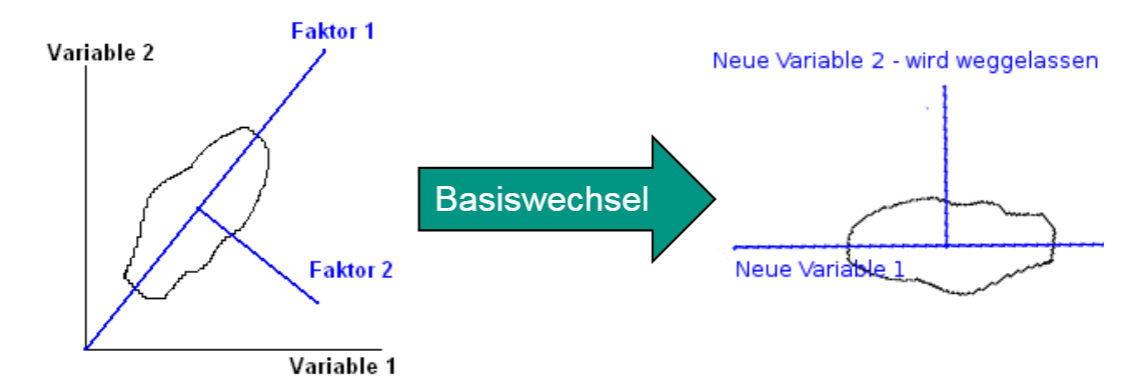
\includegraphics[scale=0.65]{Grafiken/basiswechsel.png}
PCA wird eingezeichnete Faktoren liefern, Basiswechsel liefert Situation rechts\\
G-Faktor mit PCA\\
General Faktor der intelligenz der von IQ Tests bestimmt wird\\
g-Faktor = intelligenzfaktor, der aussagt ob man dumm oder Genie ist




\subsection{Wiederholung Warscheinlichkeit}
Erwartungswert: Summe Zufallswert * Warscheinlichkeit (Würfel 1/6*1+1/6*2...)\\
Bei stetigen Zufallsvariablen: Integral Anstelle Summe \\
\\
Varianz ist Maß für Streuung, mittlere quadratische Abweichung vom Mittelwert
$v(x) = E(X-E(X))^2 = E(X^2) - E(X)^2$\\

Varianz = 0, nimmt fast nur Erwartungswert an\\
Kovarianz sehr ähnlich, Zusammenhang zwischen X und Y:\\
$C(X,y) = E[(x-E(X)(Y-E(Y))] = E(XY)-E(X)(E(Y)$\\
V(x) = C(X,X)\\
Unkorreliert = Kovarianz 0 = Stochastisch unabhängig\\
\\
Kovarianzmatrix für Zufallsvektor$ x=(x_1, x_2...)^T$

Kovarianzmatrix:
$\begin{matrix}
	C(x_1, X_1) & C(X_1, X_2) & ... & C(X_1, X_N) \\
	C(x_2, X_1) & C(X_2, X_2) & ... & C(X_2, X_N) \\
	C(x_3, X_1) & C(X_3, X_2) & ... & C(X_3, X_N) \\
\end{matrix}$

Eigenschaften: Symmetrisch, positiv-definit (Alle Eigenwerte sind positiv)\\
Hauptdiagonale = Varianzen der Komponenten von X\\


\subsection{PCA-Berechnung}
\begin{itemize}
	\item Eingabesamples $x_n:=(x_n^{(1)}, ..., x_n^{(m)})^T$
	\item Mittelwert: $\bar{x} = 1/N \sum x_n$ (Vektor)
	\item Kovarianzmatrix: $1/N \sum (x_n - \bar{x})(x_n-\bar{x})^T$ (NxN Matrix)
	\item vermutlich unwichtig:	
	\item Zunächst EINE Richtung suchen (mit größter Varianz), d.h. wir suchen Vektor p, der die $x_i$ in Skalare $y_i = px_i$ transformiert, so dass die empirische Varianz v(y) maximal ist
	\item p Nebenbedingung $\|p\|^2= pp^T = 1$
\end{itemize}

\subsection{PCA in a Nutshell}
\begin{itemize}
	\item x(t) eine multivariante Zeitreihe (Eingabesamples)
	\item PCA auf x(t) anwenden heißt:
	\item $y(t) = V^Tx(t)$
	\item $V \in O(n)$ Matrix mit den Eigenvektoren $[v_1...v_p]$, die aus Eigenwert Zerlegung der Kovarianzmatrix $\Sigma$ von x(t) bestimmt werden
	\item Wir erhalten eine Hauptkomponente $y_i(t)$ (räumlich gefilterte Zeitreihe) für jeden Iegenvektor $v_i$
	\item $y_i(t)=v_i^Tx(t)$
\end{itemize}


\subsection{PCA:Dekorrelation und Unabhängigkeit}
\begin{itemize}
	\item Entscheidender Schritt bei PCA ist Dekorrelation der ursprünglichen Dimensionen (Kovarianzen zweier verschiedener Dimensionen durch die Transformation zu Null gemacht werden)
	\item Optimal für normalverteilte! Datensätze (Nach trafo einzelne Dimensionen statistisch unabhängig)
	\item Vorteile: Parameterlos und unüberwacht->gut anwendbar ohne Strukturkenntnisse der Daten
	\item einfach berechenbar
	\item Erweiterbar um Schwächen zu lindern
	\item Probleme: (Dekorreliert Dimensionen, wenn nicht normalverteilt, Dimensionen vllt nicht unabhängig)
	\item Lösung ICA (Independend Component Analyses):
	\item Transformationsmatrix so berechnen, dass Dimensionen von vornherein maximal stochastisch unabhängig sind
	\item Algorithmus komplizierter als PCA, auch hier lineare Transformationsmatrix, die Optimierungskriterium erfüllt
	\item Optimierungskriterien durch Betrachtung der Entropie der Warscheinlichkeitsverteilungen der Dimensionen
	\item ICA Beispiel für Blind Source Seperation (Trennung eines Signals in Bestandteile von verschiedenen Quellen)
	\item Anderes Problem: PCA beachtet nicht zeitliche Strukturen der Datenpunkte
	\item Lösung: Features definieren, die eine Zeitliche Struktur enthalten, etc durch Stacking benachbarter Frames
	\item Anderes Problem: PCA versagt, wenn Hauptrichtungen der Daten nicht linear oder zueinander orthogonal sind
	\item Lösung Übergang zu nichtlinearen Transformationen, z.B. mit Kernel PCA
	\item PCA Beispiel: Gesichter erkennen mti Hilfe der PCA
	\item Ursprünglich hoher Featureraum (jeder Pixel ein Feature)
	\item Normalisierung der Gesichter nötig, anstelle Pixel Hauptkomponenten (Gesichter) berechnen und dadurch reduktion des Merkmalsvektor von 10000auf7 (z.b.)
	\item Deep Neural Netowrks: Verschachtelung mehrerer Restriced Boltzman Machines, Erkennt Parameter in Kreisdaten (PCA: nicht linear, erkennt nichts), viele Trainingsdaten nöätig
\end{itemize}


\subsection{Linear Discriminant Analysis (LDA)}
\begin{itemize}
	\item LDA Algorithmus (Fishers linear discriminant) ist linearer Kompressionsalgorithmus
	\item Basiert wie PCA auf linearem Basiswechsel
	\item Ziel anders als PCA: Trennbarkeit gewisser Klassen maximieren (nicht hohe Varianz iwe bei PCA)
	\item LDA: Überwachtet Algorithmus: Klassenzugehörigkeit der Daten bekannt!
	\item N Klassen -> N Sampledatensätze, je Daten einer Klasse
	\item LDA berechnet Transformationsmatrix, Dimensionen so Transformiert, dass neue Dimensionen nach Diskriminanz, nach Unterscheidungsfähigkeit sortiert sind
	\item erste m transformierte Dimensionen verwenden, rest ignorieren
\end{itemize}

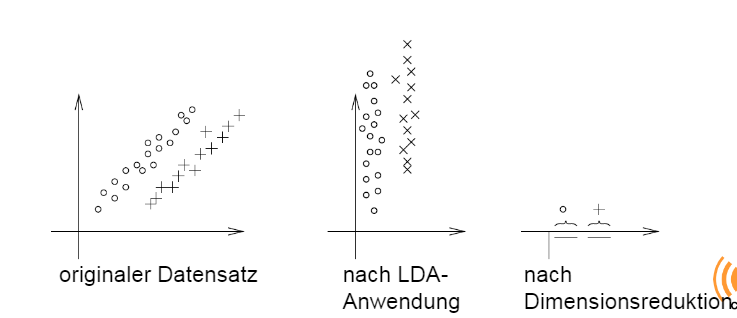
\includegraphics[scale=0.65]{Grafiken/lda.png}

\begin{itemize}
	\item Menge von Samples in 2 Klassen
	\item Annahme Beide Klassen folgen einer Gaussverteilung
	\item Projizieren Samples auf Gerade (eine Dimension), sodasss Klassentrennbarkeit maximal wird (Projektion hat Form $y=w^Tx$
	\item Projektionsvektor normiert $\|w\|^2= 1$
	\item Kriterium zur Klassentrennbarkeit könnte sein, dass Mittelpunkte möglichst weit entfernt liegen
	\item Leicht lösbar, aber nicht optimal, Klassen sollen nicht nur möglichst weit auseinander liegen, sondern niedrige Varianz haben
\end{itemize}

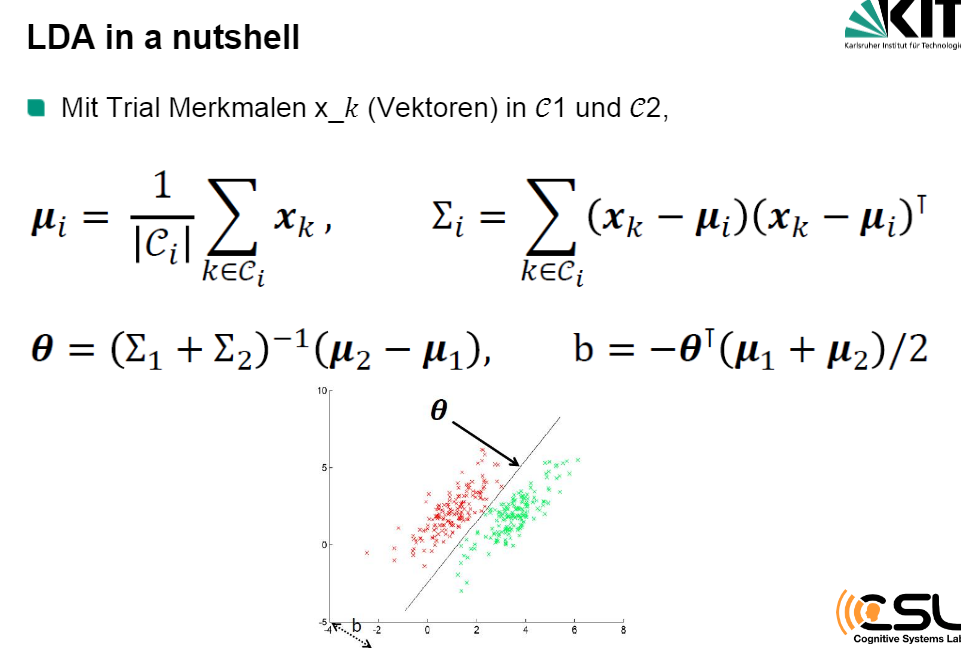
\includegraphics[scale=0.65]{Grafiken/ldainanutshell.png}

\begin{itemize}
	\item LDA mit mehreren Klassen
	\item Erweitern auf mehrere Klassen, die zu diskriminieren sind
	\item Within-class covariance
	\item Between-class covariance neu definiert
	\item Mehrere mögliche Optimierungskriterien
	\item Mittels simultaner Diagonalisierung lösbar (umständlich, nicht schwer)
	\item Ergänzende Hinweise: Anzahl Zieldimensionen muss geringer sein als die Anzahl der zu diskriminierenden Klassen
	\item LDA lässt sich auch mit Kernel Trick zu nichtlinearem Algorithmus erweitern (Kernel LDA)
\end{itemize}


\subsection{Eiugenschaften LDA}
\begin{itemize}
	\item Standardmethode zur Dimensionsreduktion in der Spracherkennung
	\item Nötig vorab Klassenzuordnungen zu haben  (Meist nur approximativ, wenn Klassenzuordnung bekannt, LDA wird PCA vorgezogen
	\item Merkregel: LDA Ist zur Verbesserung der Klassifikation gut geeignet
	\item PCA/ICA Spielen besonders dann eine Rolle, wenn überhaupt erst einmal eine gute Repräsentation des Signals gefunden werden soll
\end{itemize}


\section{Visualisierung}

\subsection{Histogramm}
\begin{itemize}
	\item Graphische Repräsentation der Verteilung von Daten
	\item Schätzen der Warscheinlichkeitsverteilung
	\item Repräsentation benachbarte Rechtecke, erzeugt über diskrete Intervalle (Bins)
	\item Anzahl Bins muss gewählt werden, abhängig vbon Anzahl Daten, Varianz in den Daten, damit Klassen gut unterscheidbar sind
\end{itemize}

\subsection{Gaussverteilungen}
\begin{itemize}
	\item Parameterfrei (Bei Histogrammen Anzahl bins, hiernichts, da gegeben)
	\item Mittelwert und Standardabweichung anfällig für Ausreißer
	\item Klassen müssen gut unterscheidbar sein
\end{itemize}


\subsection{Scatter Plots}
\begin{itemize}
	\item Diagram, das kartesische Koordinaten verwendet um 2-3 Variablen zu ziegen
	\item Punktwolken
	\item Werte werden als Positionen eingetragen 
\end{itemize}


\subsection{T-SNE}
\begin{itemize}
	\item t-Distributed StochasticNeighborEmbedding (t-SNE)
	\item Technik zur Dimensionalitätsreduktion
	\item Gut zum Visualisieren von hoch-dimensionalen Daten
\end{itemize}

\subsection{Deep Neural Networks}
\begin{itemize}
	\item Haben tausende Parameter
	\item Durch verschiedene Schichten enmtstehen komplexe Modelle
	\item Visualisierung schwer
	\item Möglichkeit: Maximieren des Outputs für ausgewähltes Neuron
\end{itemize}

\section{Mustererkennung}


\subsection{Klassifikation/Regression}
\begin{itemize}
	\item Klassifikation = Bestimmen der vorliegenden Klasse
	\item Wenn abhängige Variable sich nicht in Klassen einteilen lässt: Regression (Benzinverbrauch in Abhängigkeit PS)
	\item Auch hier Trainingsdaten um Zusammenhang zu lernen
\end{itemize}

\subsection{Mustererkennung}
Verfahren oft statistisch: Kein Wissen über Eigenschaften der Daten, auf Basis von Trainingsdatensatz-> Modell trainiert\\
Klassifikation durch Auswerten des Modells\\
Wissensbasierte Systeme:\\
Klassifikatoren müssen nicht aus trainingsdaten gelernt werden\\
Regelbasierter Entwurf (Vorab Informationen verarbeiten)

\subsection{Definitionen}
Überwachtes/Unüberwachtes lernen:\\
Klassenzuordnungen in der Lernphase unbekannt\\
Möglicherweise Klassen unbekannt\\
Strukturen in Daten finden\\
Parametrische/Nichtparametrische Modellierung:\\
Parametrische: Annahme Datenfolgen Warscehinlichkeitsverteilung, Schätze Parameter dieser\\
Nichtparametrische: Keine Annahmen über Verteilung, Direkt auf Daten



\subsection{Unüberwachtes/Überwachtes Training}
\begin{itemize}
	\item Überwacht: Für jedes Sample aus Trainingsdatensatz ist zugehörige Klasse bekannt
	\item Fürs Training gut, sehr aufwändig oft
	\item Unüberwachtes Training: Zuordnung nicht bekannt, Gesamtmenge Klassen eventuell unbekannt
\end{itemize}


\subsection{Clustering}
\begin{itemize}
	\item Unüberwachtes Lernverfahren
	\item Cluster:; Gruppe von Datenobjekten mit ähnlichen Eigenschaften
	\item Clustering = Menge der Cluster in Datensatz
	\item Clusteranalyse: Verfahren zum berechnen
	\item Kernidee: Objekte im Cluster ähnliche Eigenschaften
	\item Objekte in unterschiedlichen Cluster haben unterschiedl. Eigenschaften
\end{itemize}

\subsection{K-Means-Algorithmus}
\begin{itemize}
	\item Ziel: Bestimme Klassenstruktur von einer Menge von N Samples im D-dimensionalen Raum
	\item Anzahl Klassen K festgelegt
	\item Minimierung des quadratischen Fehlers (Fehler = Abstand zwischen Punkt und Mittelpunkt Klasse)
	\item Problem: Mittelpunkt der Klassen hängen von Klassenzuordnung ab (->nicht leicht ausrechenbar, NP-hartes Problem->iterativ ausrechnen)
	\item Ablauf:
	\item Bis zur Abbruchbedingung:
	\item Initialisiere Mittelwerte der K Klassen (fest!) beliebig
	\item Nächste-Nachbar-Klassifikation: Ordne jedes Sample der Klasse zu, deren Mittelwert es am nächsten liegt
	\item Update: Rechne auf Basis der neuen Zuordnung neue Klassenmittelwerte aus
	\item Iteration: Wenn Abbruchbedingung nicht erfüllt, gehe zur Nächsten-Nachbar-Klassifikation
	\item Mögliche Abbruchbedingungen: Feste Anzahl Iterationen, Fehler unter Schwellwert, Klassenzuordnung ändert sich nicht / nur wenig
	\item ist mit EM-Algorithmus verwandt
	\item Geringer Rechendaufwand (keine Varianzen, einfache Distanzfunktion)
	\item Oft verwendet, um initiale Mittelwerte für Gauss-Mischverteilung zu finden und danach EM-Algo anzuwenden
	\item Probleme: Konvergiert manchmal nur zu lokalem Optimum
	\item Initialisierungsschritt kritisch: Wiederholt durchlaufen in Praxis mit unterschiedlichen Startwerten
	\item Eventuell leere Klasse
	\item Keine Varianzberechnung -> Manchmal suboptimales Ergebnis
\end{itemize}


\subsection{Hierarchisches Clustern}
\begin{itemize}
	\item Devise Verfahren (Top-Down)
	\item Alle Objekte in einem Cluster, Schrittweise aufteilen
	\item Agglomerative Verfahren (Bottom-up)
	\item Jedes Objekt eigenes Cluster, schrittweise zusammenfassen
	\item Bottom-up Algorithmus:
	\item Idee: Berechne Distanzen von jedem Datenpunkt zu jedem Datenpunkt
	\item Jedes Item eigenes Cluster, Distanz Cluster = Distanz Items
	\item Fasse zwei Cluster mit geringster Distanz zusammen
	\item Errechne neue Distanzen zwischen diesem und allen anderen
	\item Wiederhole bis nur noch ein Cluster vorhanden
	\item Typische Darstellung Dendrogramm
	\item Stellt kompletten Vorgang dar, nicht nur Endprodukt
	\item Wahl der Distanzfunktion kritisch (euklidische Distanz, Manhatton distanz, maximum Distanz), ...
	\item Distanzmaße nicht immer symmetrisch
	\item Distanzkriterium linkage:
	\item Größte Distanz zwischen Items aus beiden Klassen 
	\item Kleinste Distanz zwischen Items aus beiden Klassen
	\item Durchschnitt
\end{itemize}

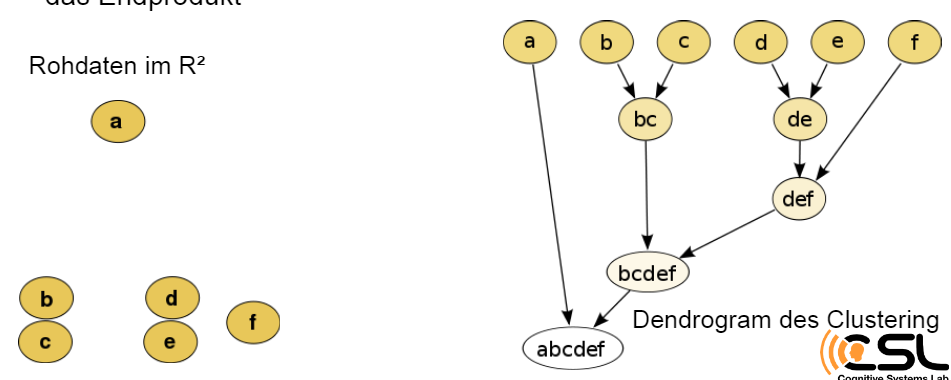
\includegraphics[scale=0.65]{Grafiken/dendrogramm.png}

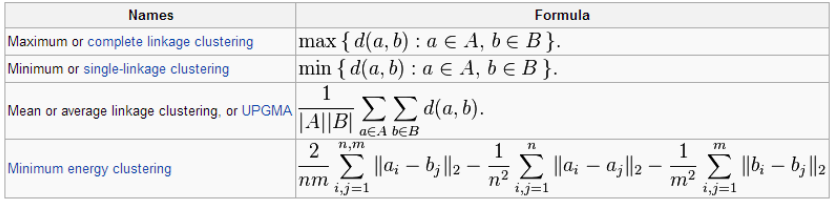
\includegraphics[scale=0.65]{Grafiken/linkage.png}


\subsection{Klassifikatoren}
Nichtparametrische Verfahren\\
\begin{itemize}
	\item Parzen Windows
	\item Keine Annahme über Verteilung
	\item Zwei Klassen c1 und c2 in einem zweidimensionalen Merkmalsraum
	\item Features sind vektoren die aus einer Vorverarbeitung entstanden sind
	\item Entscheiden, ob Punkt zu Klasse gehört: Ziehe Fenster der Größe V
	\item Zähle Samples $s_k$ jeder Klasse k, die in das Fenster V fallen
	\item Beispiel: 4 aus Klasse1, 1 aus Klasse2 -> Warscheinlich gehört zu Klasse1
	\item Formale Regel: $P(Sample x gehört zu c_k)=\frac{s_k}{\sum sk}$
	\item Problem: Fenstergröße wichtig
	\item Zu kleines Fenster: schlechte Abschätzung, Fragmentierung, Ausreißer nicht erkannt
	\item Zu großes Fenster: schlechte Auflösung
	\item Lösungsmöglichkeit: Fenstergröße von Datendichte abhängig
\end{itemize}

\begin{itemize}
	\item K-nearest Neightbors
	\item Finde k nächste Nachbar zu Sample x
	\item Bestimme häufigste Klasse unter Nachbarn
	\item Weise X dieser Klasse zu
	\item Ähnliche Probleme, geeignetes k ausschlaggebend
\end{itemize}

Nachteile von kNN/Parzen-Klassifikatoren:\\
Problem:Varianzen werden ignoriert von kNN\\
Wenn normalverteilt bietet sich Gaussklassifikator an\\
Problem:viele trainingsdaten=hoher Rechenaufwand\\
Histogramme anstelle Datensatz verwenden\\
Parametrische Klassifikator oft besser: Modell anstelle Ursprungsdaten benutzen

\begin{itemize}
	\item Histogramme zur Dichteschätzung:
	\item Ansatz: Nicht daten betrachten, sondern Histogramm aus Datenpunkten
	\item Größe bins muss festgelegt werden
	\item Zu kleine Klassen: viel erratische Struktur,m die eigtl nichjt vorhanden ist
	\item Zu große Klassen: Struktur geht verloren
	\item Skalierungsprobleme im hochdimensionalen Raum
	\item Vorteile: Rechenaufwand und Spoeicheraufwand klein
	\item Sequentielles Einfügen von Daten leicht
\end{itemize}

\subsection{Linearer Klassifikator}
\begin{itemize}
	\item x Eingabevektor
	\item Linearer Klassifikator gegeben durch:
	\item $y(x) = w^Tx+b$ Gewichtsvektor w und biasb
	\item Eingabesample x wird C1 zugeordnet wenn $y(x) \ge 0$ sonst C2
	\item Linearer Klassifikator: Featureraum wird in zwei Teile geteilt, getrennt durch Hyperebene mit Gleichung $w^Tx = 0$
	\item Falls Hyperebene, die alle Eingabevektoren fehlerlos trennt, heißen die Klassen linear separierbar (selten)
	\item Mehr als 2 Klassen:
	\item K-1 Klassifikatoren, von denen jeder eine Klasse von den Samples in allen anderen Klassen trennt: one vs the rest classifier
	\item K(K-1)/2 binäre Klassifikation, von denen jeder ein Paar von Klassen trennt: one versus one classifier
	\item Nachteil: für gewisse Klassen möglicherweise kein eindeutiges Klassifikationsergebnis, vermeiden indem man K lineare Funktionen aufstellt und Samples diesen Klassen zuordnet wenn sie "zwischen den Geraden liegen"
	\item Normalisierung:
	\item Alternative Schreibweise der Trainingsvektoren und Gewichtsvektoren (Faktor 1/l und 1/b)
	\item Verschiebt Hyperebene, sodass sie durch den Ursprung geht, Featureraum eine Dimension höher als vorher
	\item $\tilde{x}= \frac{x}{l}$ und $\tilde{w}=\frac{w}{b}$ 
	\item Klassifizierungsfunktion: $y(\tilde{x}) = w^Tx+b=\tilde{w}^T\tilde{x}$
\end{itemize}


\subsection{Training}
\begin{itemize}
	\item Bestimmung der Parameter für linearen Klassifikator
	\item LDA schon bekannt
	\item Minimierung des quadratischen Fehlers
	\item Perzeptron Algorithmus
	\item x1,..xn Trainingssamples, "klassenzubehörigkeitsvektor" ti= 0 1 0 0, wenn Sample zur 2. Klasse gehört
	\item Ziel: Fehlerfunktion definieren, diese minimieren
	\item Oft Minimierung des quadratischen Fehlers (Immer positiv, wenn minimierung durch ableiten und nullsetzen, immer Nullstelle einer linearen Funktion gesucht)
	\item betrachte Klassifikator, in dem jede Klasse durch eine lineare Funktion beschrieben wird
	\item $y_k(x) = w_k^Tx+b_k$
	\item Normalisierte Form (wie oben) und zusammenfassen aller Gleichungen in Gleichungssystem
	\item $y(x)= \tilde{W}\tilde{x}$
	\item y K-dimensionaler Spaltenvektor, W tilde ist Kx(D+1)-Matrix
	\item Ordne Sample Klasse mit größtem $y_k(x)$ zu
	\item Samples gruppieren:
	\item $\tilde{X}$ ist `(D+1)xN Matrix mit Eingabesamples als Spalten
	\item T ist KxN-Matrix, die in jeder Spalte die Zielwerte $t_n$ enthält
	\item Quadratische Fehlerfunktion
	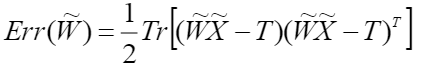
\includegraphics[scale=0.65]{Grafiken/fehler.png}
	\item Lösung=Ableitung: $\tilde{W}=T\tilde{X}_z$, $\tilde{X}_z$ ist pseudoinverse Matrix zu $\tilde{X}$
	\item Vorteile: mathematisch einfach, geschlossene Lösung des Problems
	\item Nachteile: Falsche Trennlinie: Grün richtig, lila gefunden
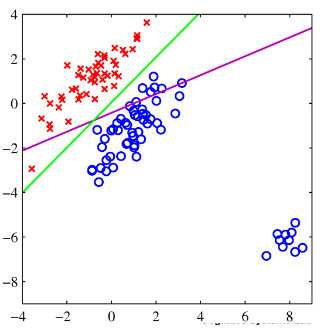
\includegraphics[scale=0.65]{Grafiken/falschetrennlinie.png}
	
\end{itemize}

Perzeptron:
\begin{itemize}
	\item Einfaches Neuronales Netzwerk
	\item Einzelnes Neuron, das +1 oder -1 ausgibt, wenn eingabevektor zur Klasse gehört
	\item Linearfall:
	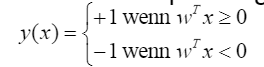
\includegraphics[scale=0.65]{Grafiken/perzeptron1.png}
	\item Alternative Formulierung für lineare Klassifikation
	\item betrachtet Eingabesamples und berechnet iterativ ein Update für Gewichtsvektor w, bis ein Abbruchkriterium erfüllt isdt
	\item w nicht in geschlossener Form gegeben
	\item Perzeptron mit obiger Klassifikationsformel ist linearer Klassifikator
	\item Grundbaustein für komplizierte neuronale Netze
	\item Leicht geänderte Definition: (Klassen C1, C2)
		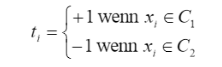
\includegraphics[scale=0.65]{Grafiken/perzeptron2.png}
	\item Wir suchen Hyperebene (w) durch Nullpunkt (kein +b Bias), sodass für möglichst viele Samples x gilt: $tw^Tx>0$, dh gleiches Vorzeichen t und wtx
	\item Fehlerbasiert: In jedem schritt hat ein Sample nur Auswirkungen auf das Training, wenn es falsch klassifiziert wird
\end{itemize}


Durchführung Perzeptron:
\begin{itemize}
	\item $x_i$ Vektor, der falsch klassifiziert wurde
	\item Abstand zur Entscheidungshyperebene: $d_i = d(x_i) = w^Tx_i$
	\item Abstand = Kosten
	\item Gradientenabstieg->Update-Regel für Gewichtsvektor (die Kostenfunktion minimiert)
	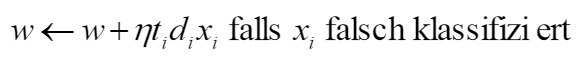
\includegraphics[scale=0.65]{Grafiken/perzeptron3.png}
	\item Gewichtsupdate durchführen bis Abbruchkriterium
	\item Falls Klassen linear separierbar, findet dieser Algorithmus eine geeignete Hyperebene in endlich viele Schritten
	\item Kann nicht konvergieren, wenn Klassen nicht separierbar
\end{itemize}

\subsection{Bayes Entscheidungstheorie}
\begin{itemize}
	\item Wir wollen Warscheinlichkeit, wie sicher Instanz zur Klasse gehört
	\item Warscheinlichkeit für eine Klasse A gegeben einen Merkmalsvektor B p(A|B) kann nicht direkt bestimmt werden
	\item P(A|B) ist die A-Posteriori Warscheinlichkeit
	\item Bayes Theorem:
	$P(A|B) = \frac{P(B|A)\times P(A)}{P(B)}$
	\item P(B|A) Warscheinlichkeit für Merkmal gegeben Klasse
	\item P(A) A priori Warscheinlichkeit für Klasse
	\item P(B) A priori Warscehinlichkeit fvür Merkmalsvektor
\end{itemize}
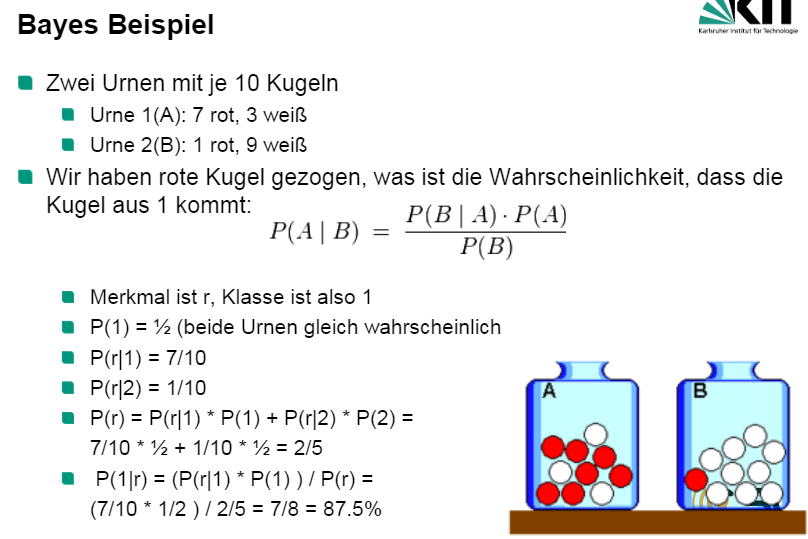
\includegraphics[scale=0.65]{Grafiken/bayes.png}
In Praxis: Wenn höchste Warscehinlichkeit gesucht wird, kann Normalisierung weggelassen werden (Ohne Teilen)\\
Dann keine echten Warscheinlichkeiten mehr

\subsection{Gaussklassifikator}
\begin{itemize}
	\item Modelliert die Verteilung von Datenpunkten mit Hilfe der Gaussverteilung
	\item Bestimmen für jede Klasse Parameter der Gaussverteilkung, die die Lage der Samples im Featureraum gut beschreibt
	\item Klassifikation = Auswertung Dichtefunktion
	\item Beliebige Verteilungen lassen sich gut als Summe von Gaussverteilungen darstellen
	\item Dichtefunktion (Gausskurve)
	\item Jede Klasse hat eigene Gausdichtefunktion
	\item Verteilungen GETRENNT modelliert
	\item Klassifikation  =Auswertung mehrdimensionaler Gaussverteilung
	\item Generatives Modell: Warscheinlichkeit, dass Modell Vektor generiert hat
	\item Diskriminatives Modell: Diskriminiert den Merkmalsraum in Entscheidungsräume
	\item Durchführung Klassifikation:
	\item Dichtefunktionen der Klassen $C_i $
	\item Schön trainierte Dichten
	\item Wir berechnen Wert jeder Guassfunktion für Eingabesample x
	\item x wird der Klasse zugeordnet, die den höchsten Wert hat
	\item Dichtewert kann weiterverwendet werden
	\item Methode geht nicht nur für Gaussverteilungen
	\item Es ergeben sich Entscheidungsregionen (nicht unbedingt zusammenhängend)
	\item Sample in Region wird in zubehörige Klasse gesteckt
\end{itemize}

\begin{itemize}
	\item Training für Gaussklassifikator
	\item Suche geeignete Mittelwert und Kovarianzmatrix für Samples
	\item Wir wählen so, dass abgeschätze Verteilung der Samples maximale Warscheinlichkeit hat
	\item 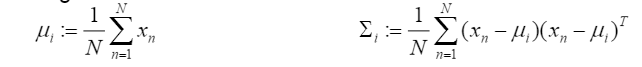
\includegraphics[scale=0.65]{Grafiken/traininggauss.png}
	\item Maximum Likelihood Abschätzung
	\item Sehr einfach unaufwendig, nicht iterativ, für jede Klasse getrennt durchführen
	\item Für alle Klassen Mittelwert und Varianz => Gaussklassifikator
	\item Bei wenigen Trainingsdaten: Nur Diagonalwerte der Kovarianzmatrizen trrainieren, andere Werte 0
	\item Alternative Methode: Diskriminatives Training: Klassifikationsfehler möglichst klein halten, aufwändig
\end{itemize}


\subsection{Gauss-Mischverteilungen}
Man benutzt mehrere Verteilungen um genauere Approximationen zu erhalten\\
beim Test nicht eine Gaussverteilung ausgewertet, sondern mehrere\\
Jede Verteilung hat Gewicht
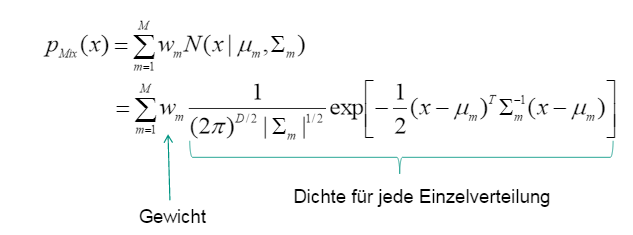
\includegraphics[scale=0.65]{Grafiken/dichtefunktionmisch.png}

Vor und Nachteile:\\
Flexibilität\\
Man kann Anzahl Verteilungen von Komplexität der Klasse abhängig machen\\
Parameter Tying: Man kann Parameter sparen (Wenn zuwenig Trainingsdaten)\\
Wir können identische Mischverteilungen mit unterschiedlichen Gewichtne für mehrere Klassen benutzen\\

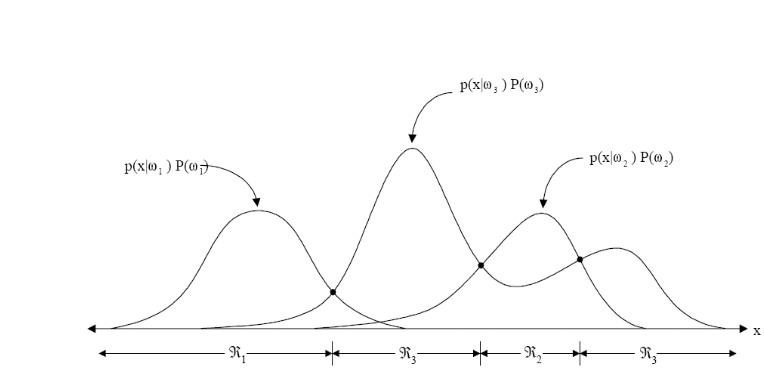
\includegraphics[scale=0.65]{Grafiken/entscheidungsregionenmisch.png}

Anzahl Verteilungen muss gut gewählt sein! (2Phenome, 2Gaussmischverteilungen)

\subsection{Training von Gauss Mischverteilungen}
\begin{itemize}
	\item Vorhin: Einzelne Gaussverteilungen durch Maximum Likelihood Abschätzungfen von Mittelwert und Kovarianz trainierbar
	\item Problem: Wie viele wollen wir trainieren, welche Samples gehören zu welcher Verteilunge?
	\item Doppeltes Optimierungsproblem:
	\item Optimale Form der Gaussverteilungen hängt von den zugeordneten Samples ab
	\item Zurodnung Samples hängt von Verteilungen ab
	\item Zuordnung ist eine probabilistische Zuordnung
	\item WIeder Maximum Likelihood Training
	\item Doppeltes Optimierungsproblem: Keine analytische Lösung
	\item Iterativer Algorithmus, der Zuordnung und Verteilungsparameter schrittweise abwechselnd optimiert (EM, Expectation maximization) Algorithmus
	\item Aufwändig, Initialisierung: K-Means-Ago
	\item Annahme: Gewünmschte Anzahl der Gaussglocken bekannt
	\item EM-Algo ist allgemeines Verfahren zur Bestimmung von Maximum Likelihood Schätzwerten beio probabilistischen Modellen
	\item Durchführung hängt von Zusammenhang ab
	\item Für Gauss Mischverteilungen:
	\item Grundidee: Zweistufig iterativ
	\item Estimation Step: Probabilistische Zuordnung der Samples zu Gaussverteilungen berechnet
	\item Maximization Step: Parameter der Modelle werden so optimiert wie vorhin
	\item Warscheinlichkeit der Beobachtung wird maximiert unter Annahme der Zuordnung von SChritt 1
	\item Abwchselnd ausführen, bis Erwartungswert nicht oder nur noch kaum ändert
	\item Dann lokales Maximum gefunden
	\item Maximization-Step: Jede Gaussverteilung abgeschätzt wie immer, jedes Sample wird gewichtet, GEwicht ist Zuordnungswarscheinlichkeit zur Verteilung
	\item In jedem Schritt erhöht EM die log-likelihood Funktion (quasi Gesamtwarscheinlichkeit) der Trainingssamples, Abbruchkriterium wenn log-likelihood sich nicht mehr stark ändert (oder mit etwas Erfahrung feste Zahl Iterationen)
\end{itemize}

\subsection{Suppor Vector Machines}
\begin{itemize}
	\item Beruht auf 3 Tricks:
	\item Finde Hyperebene (trennfläche in 2 Klassen). Hyperebene soll maximalen Abstand zu denjenigen Vektoren haben, die der Ebene am nächsten liegen
	\item Nur Trainingsvektoren betrachten, die am nächsten an der Hyperebene liegen (Stützvektoren, Support Vektors)
	\item Wenn Daten nicht linear separierbar, transformiere Merkmalsraum mit Kernel-Trick
	\item Abstand heißt margin
	\item Generalisierungsfähigkeit: Unbekannte Datenpunkte können besonders gut klassifiziert werden
	\item Zwei Klassen, Zielwerte $t_n$ 1 oder 0 je nach Klasse
	\item Margin ist Minimum aller Abstände zur Trennebene
	\item Wir wollten größte Margin, es ergibt sich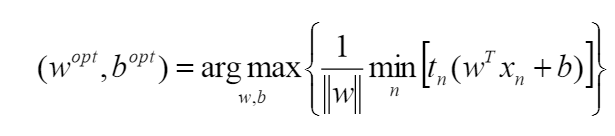
\includegraphics[scale=0.65]{Grafiken/margin.png}
	\item Schlecht analytisch zu fassen, duale Repräsentation
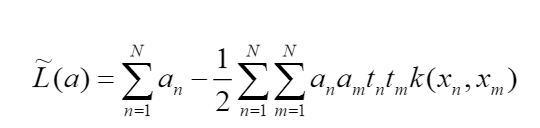
\includegraphics[scale=0.65]{Grafiken/dualerep.png}
	\item Kernel Funktion vorerst $k(x,x')= x^Tx'$
	\item Zu maximieren sind Parameter $a_n$ (ist effizient, Standardverfahren)
	\item Neue Datenpunkte klassifizieren, in dem wir einsetzen:
	\item $w=\sum a_nt_nx_n$
	\item 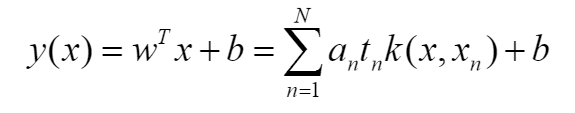
\includegraphics[scale=0.65]{Grafiken/linearesvm.png}
	\item Es kann gezeigt werden, dass entweder $a_n=0$, dann Sample irrelevant oder $t_ny_n=1$, dann liegt Punkt genau auf Rand (nur wenig meist) = Support Vektors
	\item Sparsity: Nur Support Vektors für Klassifikation benötigt: Sehr effizient
\end{itemize}

\subsection{Nichtlineare Klassifikation}
Anstelle von Hyperebene nichtlineare Trennfunktion nehmen, sehr aufwändig\\
Trick: Wir bilden ab auf hochdimensionalen Featureraum, in dem Trennfunktion linear ist->linear Trennen\\
Problem: Aufwand um Abbildungsfunktion $\Phi$ zu berechnen sehr hoch\\
Aber Um SVM zu trainieren und um die Klassifikation durchzuführen brauchen wir lediglich die Werte der Kernelfunktion $k(x,x_n) = \Phi(x) \Phi(x_n)$\\
Geeignetes $\Phi$, viel einfacher zu berechnen als Funktion selbst\\
Dies ist Kernel Trick\\
\\
Zusammenfassung: Haupteigenschaften SVM:\\
Featureraum: Klassifikation nichtlinearer Trennung wird durchgeführt, indem die Daten in einen Featureraum abgebildet werden, wo sie linear trennbar sind. Wegen des Kernel tricks ist die Komplexität handhabbar.\\
Sprasity: Zur Klassifikatioon nur wenige Trainingssamples wichtig, die am nächsten der Trennhyperebene liegen\\
Maximum Margin: Das Training beruht auf dem lerntheoretisch optimalen Margin-Kriterium\\ \\
In Praxis fast nie linear trennbar, slack variables: einzelne Datenpunkte dürfen falsch klassifiziert werden

\subsection{Regression}
\begin{itemize}
	\item Nicht Zuweisen eines Samples zu einer Klasse, sondern abbilden auf kontinuierlich abhängige Variable
	\item Interpolation vs Extrapolation: Interpolation innerhalb Bereichs gesicherter Werte, Extrapolation über den gesicherten Bereich hinaus
	\item Lineare Regression: Annahme, linearer Zusammenhang zwischen unabhängiger Variable (Merkmal) und der abhängigen Variable
	\item Linear, da erste Potenz der Regressionskoeffizienten
	\item 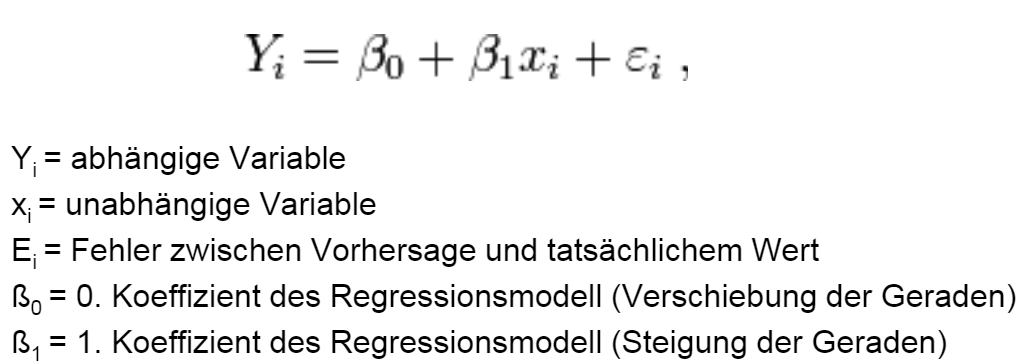
\includegraphics[scale=0.65]{Grafiken/linregression.png}
	\item Zu bestimmen sind $\beta_0, \beta_1$ und Fehler E
	\item Parameter für Regressionsmodell nicht bekannt: schätzen $y_i=a+bx_i+e_i$
	\item Quadratrischen Fehler minimieren:
	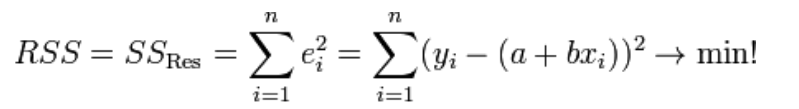
\includegraphics[scale=0.65]{Grafiken/quadratfehler.png}
	\item Man erhält:
	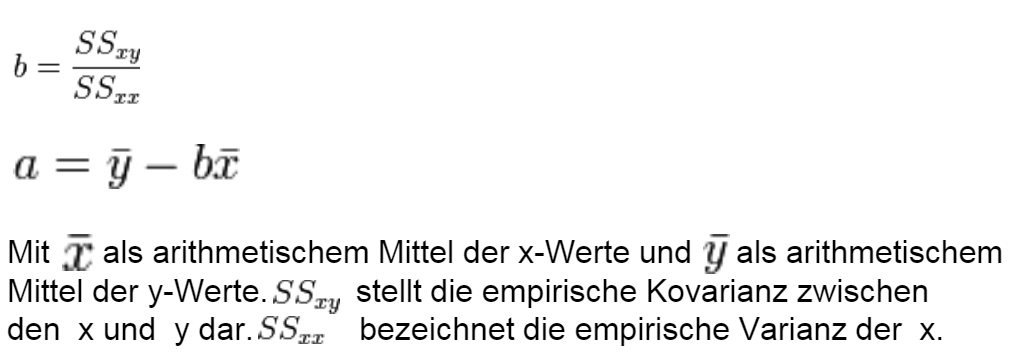
\includegraphics[scale=0.65]{Grafiken/lsglinreg.png}
	\item In Biosig normalerweise multiple Regression: mehrere unabhängige Variablen $Y=\beta_0+\beta_1x_1+\beta_2x_2+...+\epsilon$
	\item Zur Berechnung lineares Regressionsmodell auf mehr Dimensionen erweitern
	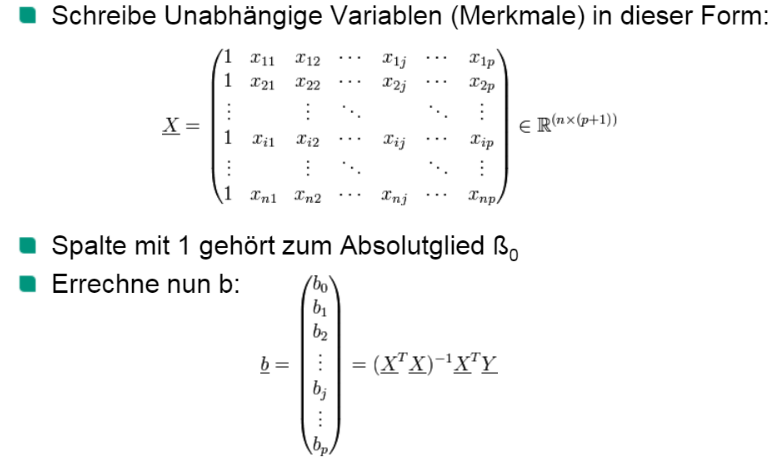
\includegraphics[scale=0.65]{Grafiken/multipreg.png}
	\item Dieser Schätzer ist nach dem Gauß-Markow-Theorem der beste lineare unverzerrte Schätzer
	\item Mit dem errechneten b-Vektor können nun Schätzwerte für neue Merkmale errechnet werden 
	
\includegraphics[scale=0.65]{Grafiken/neuemerkmale.png}
	\item Lineare/Multiple Regression einfachste Regressionsmodelle, viele andere existieren: Logistische Regression, Support Vector Regression
\end{itemize}





%__________________________________BENNE



\section{11 - HMM (Hidden Markov Models)}
	\begin{itemize}
		\item Modellieren Sequenz von Datenpunkten
		\item benötigen zugrundeliegendes state modeling
		\item oft zusammen mit GMMs verwendet
	\end{itemize}
	
\subsection{Sequenzmodellierung und State-Modelierung}
	\begin{itemize}
		\item Sequenzmodellierung ist in typischer Signalverarbeitungskette letzte Schritt nach Datenverarbeitung und State Modeling 
		\item Klassifikation und Sequenzmodellierung eng miteinander verbunden
	\end{itemize}

\subsection{Dynamic Time Warping}
	\begin{itemize}
		\item einfaches Verfahren zum Vergleich von Sequenzen
		\item Algorithmen in der HMM-Modellierung sehr ähnlich zu DTW
		\item Wir haben: Aufnahmen von Sprachsignalen - Trainingsdaten (Beispielaufnahmen mit bekanntem Inhalt) + Testdaten (Aufnahmen mit unbekanntem Inhalt)
		\item Ziel: Wir wollen die Distanz einer unbekannten Sequenz und einer Beispielsequenz berechnen
		\item Frame für Frame-Vergleich Probleme: Signale sind unterschiedlich lang + Anfang und Ende der Äußerung nicht bekannt
		\item Faggot-Lösung: Lineares Alignment - für fast alle Zwecke aber viel zu unflexibel
		\item Killer-Lösung: DTW
				\begin{itemize}	
					\item basiert auf Prinzip des dynamischen Programmierens (DP) bzw. der minimalen Editierdistanz
					\item Pfade durch eine Matrix von möglichen Zuordnungen berechnet
					\item Ergebnis: Distanzmaß zwischen den beiden Äußerungen
				\end{itemize}
	
		\item Ziel: Finde Distanz zwischen den beiden Äußerungen (je niedriger desto besser)
		\item Problem: Alle Pfade müssen betrachtet werden um den Besten zu finden
		\item Lösung:
				\begin{itemize}
					\item Berechne für jede Zeit $t$ die kumulativen Distanzen $\alpha(s,t)$, die die Distanz der Teiläußerungen bis zu den Zuständen q(s,t) (s=,1,..,S)  beschreiben
					\item Die Distanzen für Zeitpunkt t+1 berechnen sich iterativ aus denen für Zeitpunkt t und hier wird Minimierung der Distanz durchgeführt
				\end{itemize}
					\item Benötige Distanzmaß $d(s,t)$ für den beobachteten Frame t und den Referenzframe s (z.B. euklidische Distanz)
 		\end{itemize}
 		\centering
 		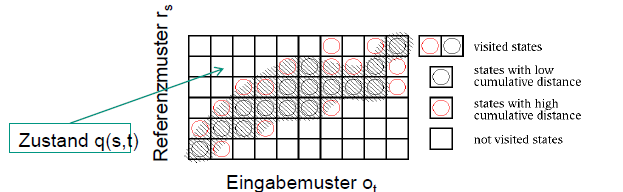
\includegraphics[scale=0.65]{Grafiken/DTW_Beispiel.png}
 		
 		\begin{itemize}
 			\item Welche Übergänge zwischen Frames sind möglich? Was haben sie für Distanz-Kosten?
 			\item Erlaubt sind überlicherweise:
 				\begin{itemize}
 					\item Ersetzung: Kosten = d(.,.) (praktisch immer > 0)
 					\item Einfügung/Auslassung eines Frames: Kosten können in der Praxis ignoriert werden
 					\item Einfügung/Auslassung mehrerer Frames: evtl. Extra-penalty, max. Zahl von Frames, die ausgelassen werden dürfen
 				\end{itemize}
 		\end{itemize}
\vspace{5px}
\flushleft Ablauf des Algorithmus:
 			\begin{itemize}
 				\item Initialisierung: Beginne bei Startzustand $q(0,0)$, $t:=0$, $\alpha(0,0):=d(0,0), \alpha(x,0)=\infty$
 				\item Für jeden Zustand $q(s,t)$:
 					\begin{itemize}
 						\item Betrachte jeden erlaubten Zustandsübergang $q(s',t-1) -> q(s,t)$
 						\item Finde min. Distanz zu $q(s,t)$
 						\item Bis Teildistanz $\alpha(s,t)$ einen gewissen Grenzwert überschreitet
 					\end{itemize}
 				\item weitere Einschränkungen des Suchraums denkbar
 				\item Komponenten der Zustandsmatrix Schritt für Schritt berechenbar (zeiteffizient + speichereffizient)
 			\end{itemize}
 		\begin{itemize}
 			\item Anwendung in der Spracherkennung
 			\item z.B. heute noch praktisch bei der Erkennung von sehr kleinen Vokabularen
		\end{itemize} 	
		
\vspace{5px}
\flushleft Probleme bei Unterscheidung einer kleinen Menge von Wörtern:
		\begin{itemize}
			\item benötigt eine Endpunktdetektion
			\item wird sehr ineffizient wenn viele Trainingsbeispiele vorhanden sind - großes Vok. braucht extrem viele Trainingsbeispiele
			\item Trainingsdaten können nicht zwischen verschiedenen Referenzen geteilt werden
			\item Erkennung unbekannter Wörter ist nicht möglich
			\item ungeeignet für kontinuierliche Sprache
			\item sehr kurze Wörter sind schwer zu trainieren
		\end{itemize}
	$\Rightarrow$ Andere Methode wird benötigt die es ermöglicht, kleinere Einheiten (Silben, Phoneme) zu trainieren und zu erkennen 		

\subsection{Markov-Modelle}
Sprachproduktion als stochastischer Prozess
	\begin{itemize}
		\item Beobachtungen zur Sprachproduktion:
		\begin{itemize}
			\item das gleiche Wort/Phonem hört sich jedesmal anders an
			\item in einem gegebenen Zustand können verschiedene Laute mit 		unterschiedlicher Wahrscheinlichkeit beobachtet werden
			\item der Produktionsprozess kann Übergänge aus einem Zustand in einen anderen machen, aber nicht alle denkbaren Übergänge sind möglich, zumindest nicht gleich wahrscheinlich
		\end{itemize}
		\item Sprachprozess befindet sich zu jedem Zeitpunkt in einem Zustand
		\item In jedem Zustand werden Laute ausgegeben entsprechend einer gewissen Wahrscheinlichkeit: Emissionswahrscheinlichkeit
		\item Die Übergänge zwischen Zuständen erfolgen auch entsprechend einer gewissen Wahrscheinlichkeitsverteilung: Übergangs- oder Transitionswahrscheinlichkeiten
		\item Markov-Modelle:
			\begin{itemize}
				\item Es gibt eine diskrete Zustandsmenge ${s_1, ... ,s_N}$
				\item Wir beobachten eine probabilistische Zustandssequenz $O = (o_1,...,o_T), o_i \in  {1,...,N}$
				\item Markov-Annahme: Wahrscheinlich, dass wir zum Zeitpunkt t in einem gewissen Zustand sind, hängt nur von vorhergehendem Zustand ab
				\item Verteilung soll stationär (zeitunabhängig) sein
			\end{itemize}
	\end{itemize}
	
\subsection{Hidden-Markov-Modelle}
Markov-Modelle und Spracherkennung
	\begin{itemize}
		\item Zustand $<=>$ Beobachtung
		\item In der Sprache haben wir aber ein Kontinuum an möglichen Tokens (typischerweise Sprachsignalframes), die endlich vielen Zuständen (Phonemen) zugeordnet werden sollen
		\item In der Sprache sind die Zustände versteckt (hidden)
	\end{itemize}
	
Hidden-Markov-Modelle (HMM) 
	\begin{itemize}
		\item sind ein doppelter stochastischer Prozess
			\begin{itemize}
				\item Zustandsabfolge probabilistisch
				\item Jeder Zustand emittiert seine Beobachtung: Diese Emission ist ebenfalls probabilistisch
				\item Zustandsfolge ist versteck (hidden)
			\end{itemize}
		\item Sind Markov-Modelle (1. Ordnung)
			\begin{itemize}
				\item Wahrscheinlichkeiten für den Eintritt in den nächsten Zustand hängen nur vom aktuellen Zustand ab
			\end{itemize}
		\item Nichtbeobachtbarkeit der Zustandsfolge hat eine Reihe von Konsequenzen		
			\begin{itemize}
				\item Sprachdekodierung mit HMMs: Anhand der Beobachtungen auf eine mögliche Zustandssequenz rückschließen (dabei wird man nie die exakte Lösung erhalten, sondern nur eine mit höchster Wahrscheinlichkeit)
				\item Training von HMMs: Kennen zwar die durchlaufene Zustandsfolge, aber nicht die Zeitpunkte der Zustandsübergänge
			\end{itemize}
			\centering 
			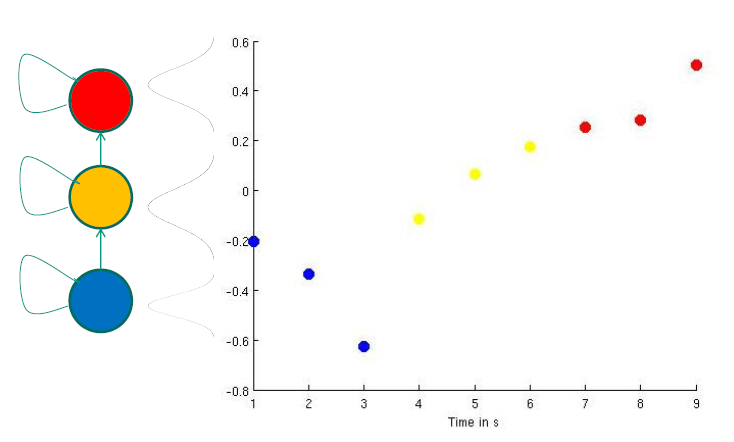
\includegraphics[scale=0.5]{Grafiken/hmm-darstellung.png}
	\end{itemize}

Formale Definition:
	\begin{itemize}
		\item HMM $\lambda = (S,\pi, A,B,V)$
		\item $S={s_1,...,s_N}$ - Menge aller möglichen Zustände
		\item $\pi$: $\pi(s_i) = P(q_1 = s_i)$ - Anfangsverteilung bei t=1
		\item $A=((a_{ij})), 1 \leq i, j \leq n$ - Matrix von Übergangswahrscheinlichkeiten
		\item $B=(b_i)$ - Vektor von Ausgabewahrscheinlichkeiten, d.h. $b_i(v)=P(o_t = v | q_t = s_i)$. Dabei ist $v \in V$
		\item V - Vokabular, Menge der Ausgabesymbole (diskret oder kontinuierlich)
	\end{itemize}

Diskrete HMMs:$V = {x_1,x_2, ...,x_v}$, dann sind die $b_i$ diskrete Wahrscheinlichkeiten


Kontinuierliche HMMs: $V=R^d$, dann sind die $b_i$ stetige Wahrscheinlichkeitsdichten

\begin{itemize}
	\item Für die Anfangswahrscheinlichkeiten gilt $\sum_i \pi(s_i) = 1$. Vereinfachend nimmt man oft einfach: $\pi(s_1) = 1 \enspace , \enspace \pi(s_j) = 0 \enspace , \enspace j \neq 0$, d.h. es gibt einen ausgezeichneten Startzustand)
	\item Es gilt $\sum_j a_{ij} = 1$ für alle i und meistens ist $a_{ij} = 0$ für die meisten Folgezustände j
\end{itemize}
Die Struktur eines HMMs nennt man Topologie:
	\begin{itemize}
		\item Lineares Modell:  \\ 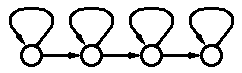
\includegraphics[scale=0.3]{Grafiken/hmm-struktur.png} 
		\item Links-nach-Rechts-Modell: \\ 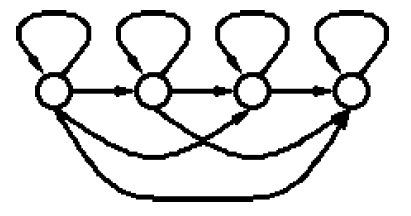
\includegraphics[scale=0.2]{Grafiken/hmm-lnr.png} 
		\item Alternative Pfade: \\ 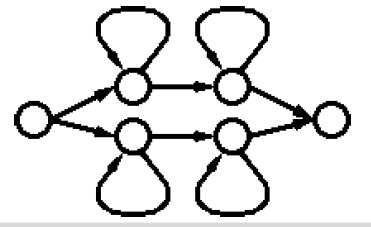
\includegraphics[scale=0.2]{Grafiken/hmm-ap.png}
		\item Bakis model (lin. Modell + kann je 1 Zustand übersprungen werden): \\ 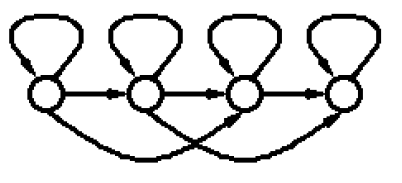
\includegraphics[scale=0.2]{Grafiken/hmm-bakis.png}   
		\item Ergodisches Modell (Jeder Zustand ist von jedem anderen Zustand erreichbar): \\
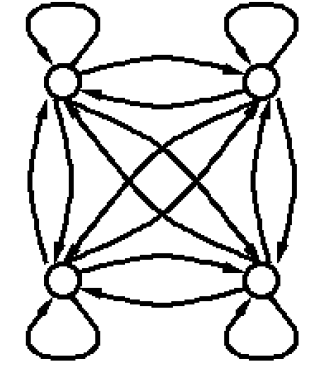
\includegraphics[scale=0.2]{Grafiken/hmm-em.png} 
	\end{itemize}

HMM-Theorie kennt drei Hauptaufgaben: Evaluationsproblem, Dekodierungsproblem, Optimierungsproblem

Evalutationsproblem: Berechne die Wahrscheinlichkeit der Beobachtung $P(O|\lambda)$
	\begin{itemize}
		\item Entspricht der Durchführung des DTW-Algorithmus
		\item Forward-Algorithmus löst dieses Problem
		\item Herausforderung: Wir müssen die Wahrscheinlichkeit der Beobachtung entlang aller möglichen Pfade berechnen
		\item Sehr aufwendig - Finden effizienter Algorithmen
		\item Frage: Wie summieren wir die Wahrscheinlichkeiten entlang aller möglichen Pfade effizient auf?
		\item Lösung: Ansatz ist wie beim dyn. Programmieren:
			\begin{itemize}
				\item Berechne iterativ für jeden Frame und jeden Zustand die Vorwärts-Teilwahrscheinlichkeiten (forward probabilities) $\alpha$
				\item Dann ergibt sich eine Matrix A der Vorwärtswahrscheinlichkeiten \\ 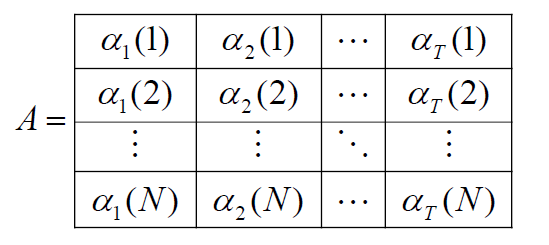
\includegraphics[scale=0.2]{Grafiken/hmm-fa-A.png}
				\item $\alpha_t(j)$ bezeichnet die Wahrscheinlichkeit, bei gegebener Teilbeobachtung zum Zeitpunkt t im Zustand j zu sein. Zur Berechnung iteriert man über die Zeit:
				\item Init: $\alpha_1(j) = b_j(o_1) \pi(s_j)$
				\item Induktion: $\alpha_t(j) = b_j(o_t) \cdot \sum_{i=1..n} a_{ij} \alpha_{t-1}(i)$ 
				\item Ergebnis: $p(o_1,o_2,...,o_T|\lambda) = \sum_{j=1..n} \alpha_T(j)$
				\item Komplexität: $O(N^2T)$
			\end{itemize}
	\end{itemize}

Dekodierungsproblem: Berechne die wahrscheinlichste Zustandsfolge bei der gegebenen Beobachtung $(q_1^*,...,q_{t-1}^*,q_t^*) = arg \max_{q_1,...,q_t} P(q_1,...,q_t|O,\lambda)$. Viterbi-Algorithmus:
	\begin{itemize}
		\item Definiere: $z_t(j) := \max_{q_1,...,q_{t-1}} P(q_1,...,q_{t-1}, q_t = j, o_1,...,o_t)$
		\item $z_t$ ist die maximale Wahrscheinlichkeit (maximiert über alle Zustandsfolgen bis Zeitpunkt t), mit der bei der gegebenen Teilbeobachtung zum Zeitpunkt t der Zustand j erreicht wird
		\item Man kann $z_t(j)$ iterativ berechnen, indem man alle möglichen Vorgängerzustände betrachtet und maximiert: \\
			$z_t(j) = \max_i z_{t-1}(i) \cdot a_{ij} \cdot b_j(o_t)$\\
			$z_1(j) = \pi(s_j) \cdot b_j(o_1)$
		\item Ergibt sich eine Matrix Z, ähnlich wie beim Forward-Algorithmus \\
		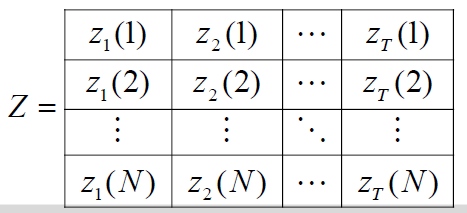
\includegraphics[scale=0.2]{Grafiken/viterbi-algo.png}
		\item Rechenaufwand: $O(N^2T)$
		\item Außerdem speichern wir für jeden Zustand den optimalen Vorgängerzustand: $r_t(j) = argmax_t (z_{t-1}(i) a_{ij})$
		\item Wenn alle $z_t$ und $r_t$ berechnet sind, kann Rückwärtszeiger $r_t$ benutzt werden, um die gesuchte optimale Zustandsfolge zu berechnen
		\item Beginne beim letzten Zeitpunkt T und suche den wahrscheinlichsten Zustand. Dann gehe entlang der Rückwärtszeiger schrittweise zurück: \\
		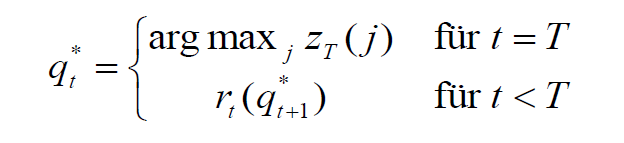
\includegraphics[scale=0.2]{Grafiken/viterbi-algo-qt.png}
	\end{itemize}

Optimierungsproblem: Finde ein HMM $\lambda^{'}$, so dass $P(O|\lambda^{'})> P(O|\lambda)$ (Ein gegebenens HMM $\lambda$ soll verbessert werden)
	\begin{itemize}
		\item Welche Parameter können trainiert werden: Übergangswahr., Emissionswahr., Anfangswahr.
		\item Probleme bei der Optimierung: unbekannt zu welchem Zeitpunkt wir in welchem Zustand sind, Wahrscheinlichkeit berechenbar dass zu Zeitpunkt t im Zustand $s_j$ (diese Information können wir zur Gewichtung nutzen)
		\item Lösung des Optimierungsproblem besteht aus 2 Schritten:
		\item Estimation Step: Berechne die Zuordnungswahrscheinlichkeit von Trainingsdaten zu HMM-Zuständen
			\begin{itemize}
				\item Trainingsbeobachtung $O=(o_1,...,o_T)$
				\item für jedes Sample die Wahrscheinlichkeit berechnen, dass es einem gewissen HMM-Zustand zuzuordnen ist
				\item für jede Kombination von aufeinanderfolgenden Samples die Wahrscheinlichkeit berechnen, dass sie einem gewissen Zustandsübergang zuzuordnen sind
			\end{itemize}
		\item Maximization Step: Optimiere die Parameter von Emissionswahrscheinlichkeiten, (Übergangswahrscheinlichkeiten und Anfangswahrscheinlichkeiten)
	\end{itemize}
 
Forward-Backward-Algorithmus:
	\begin{itemize}
		\item Berechnet die Zuordnungswahrscheinlichkeiten von Trainingsdaten zu HMM-Zuständen, löst also den Expectiation Step
		\item Betrachten wir eine Beobachtung $o=(o_1,...,o_T)$
		\item Gesucht sind 2 Parameter:
			\begin{itemize}
				\item $Y_t(j) = P (q_t=j|o_1,...,o_T,\lambda)$ ist die Wahrscheinlichkeit, dass der Beobachtungsvektor $o_t$ zum Zustand j gehört
				\item $\xi_t(i,j) = P (q_t=i,q_{t+1}=j | o_1,...,o_T,\lambda)$ ist die Wahrscheinlichkeit, dass zum Zeitpunkt t im Zustand i befinden und dann in den Zustand j übergehen
			\end{itemize}
		\item Beide Wahrscheinlichkeiten hängen von der gesamten Beobachtung o ab
		\item Berechnung von $y$ und $\xi$
			\begin{itemize}
				\item Forward-Algorithmus berechnet die Wahrscheinlichkeit, nach der Teilbeobachtung $(o_1,...,o_t)$ also zum Zeitpunkt t im Zustand j zu sein
				\item Backward-Algorithmus berechnet die Wahrscheinlichkeiten im Zustand j zu sein und dann die Teilbeobachtung $(o_{t+1},...,o_T)$ zu machen
				\item Kombination der beiden ergibt Forward-Backward-Algorithmus, der $Y_t(j)$ berechnet
				\item Berechne $P(q_t=j|o_1,...,o_T,\lambda)$ druch Aufspaltung in Forward-Teil (bis Zeit t) und Backward-Teil (nach Zeit t).
				\item $\alpha_t(j) := P(q_t=j,o_1,...,o_t|\lambda)$ \\
					  $\beta_t(j) := P(q_{t+1}=j,o_1,...,o_T|\lambda)$ \\
					  $\Rightarrow P(q_t=j|o_1,...,o_T,\lambda) = \alpha_t(j) \cdot  \beta_t(j)$. Anwendung der Bayes-Regel ergibt: \\ \vspace{3px}
				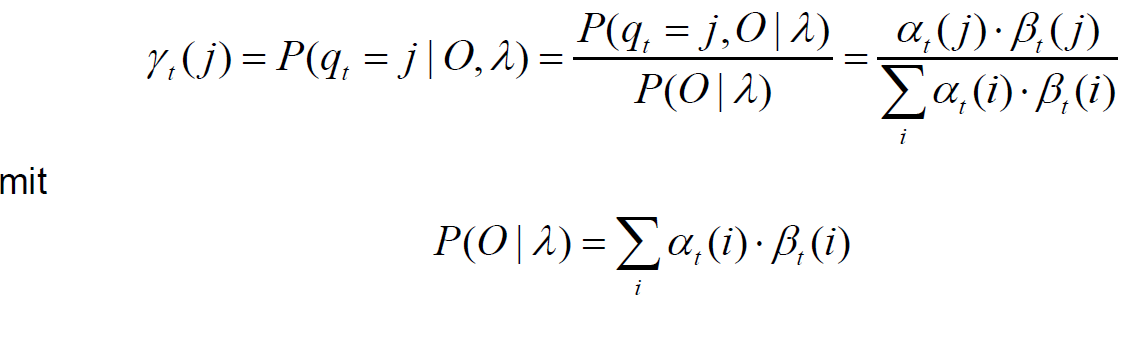
\includegraphics[scale=0.2]{Grafiken/forward-backward-algo.png}	  	
				\item $\beta_t$ können ähnlich wie die $\alpha_t$ rekursiv berechnet werden, aber rückwärts:
					\begin{itemize}
						\item Init: $\beta_T(i) = 1$ für alle Zustände i
						\item Induktion: $\beta_t(t) = \sum_{j=1..n} a_{ij} b_j (o_{t+1})\beta_{t+1}(j), \enspace t=T-1,..., 1$
						\item Durch Aufsummieren: $\Rightarrow p(o_{t+1},o_{t+2},...,o_T|\lambda) = \sum_{j=1..n} \beta_T(j)$
					\end{itemize}			
				\item[] 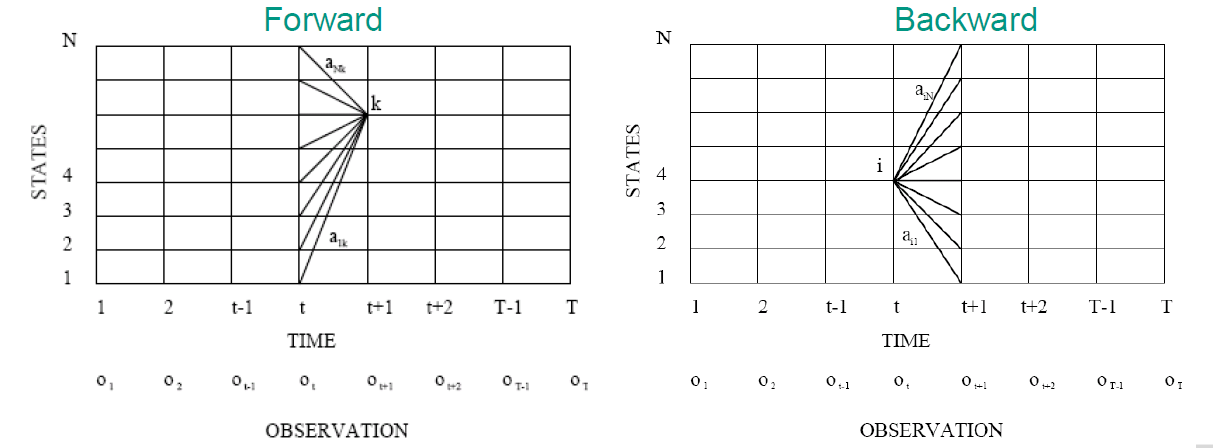
\includegraphics[scale=0.25]{Grafiken/forward-backward-beta.png}	  		 		\item $\xi_t(i,j)$: auch mit Forward-Backward-Algorithmus $\xi_t(i,j) = P(q_t = i,q_{t+1} = j|O,\lambda)$
				\item[] 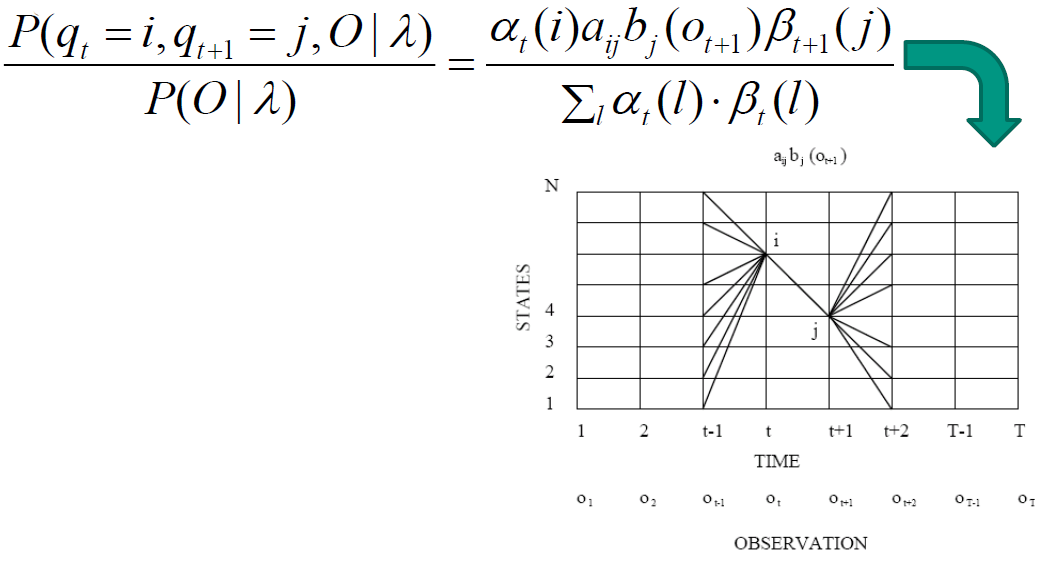
\includegraphics[scale=0.2]{Grafiken/xis.png}
			\end{itemize}
	\end{itemize}

\underline{Optimierung des HMMs:}
	\begin{itemize}
		\item Trainingsdaten den HMM-Zuständen und Zustandsübergängen zugeordnet
		\item Das war der Expectation Step des Algorithmus
		\item Führe nun Maximierung der HMM-Ausgabewahrscheinlichkeit durch (Maximization Step)
		\item Zuordnung der Samples zu HMM-Zuständen, gegeben durch $\alpha_t(j),\beta_t(j),Y_(j)$
		\item Falls Emissionswahrscheinlichkeiten durch Gauss-Mischverteilungen modellieren, dann verwende EM-Algorithmus zum Training
	\end{itemize}
	
\underline{Optimierung der Emissionswahrscheinlichkeiten:} \\
Betrachten Emissionswahrscheinlichkeiten $B^{'}=(b_1^{'},...,b_N^{'})$ bei diskretem Ausgabealphabet V. Zu jedem Zustand i = 1,...,N gehört eine Verteilung $b_i$, so dass $b_i(v_k) \in  [0,1]$ die Wahrscheinlichkeit angibt im Zustand i die Beobachtung $v_k$ zu machen. \\
Danach werden die $b_i^{'}$ bestimmt: 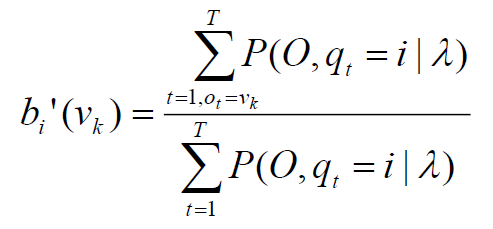
\includegraphics[scale=0.2]{Grafiken/bis.png}\\
Das heißt, $b_i^{'}(v_k)$ entspricht dem Anteil der Emissionen von $v_k$ an der Gesamtzahl der "Besuche" von Zustand i.
	
	
\underline{Optimierung der Übergangswahrscheinlichkeiten:} 	
	\begin{itemize}
		\item $sum_{t=1..T-1} \xi_t(i,j)$ ist der Erwartungswert der Anzahl der Transitionen von i nach j
		\item Der neue Wert $a_{ij}^{'}$ ist der Anteil der Transitionen von i nach j, normalisiert durch die Gesamtzahl der Transitionen (=Besuche) von i 
		\item Summiere über alle Zeitpunkte t=1,...,T: $a_{ij}^{'} = \frac{\sum_t \xi_t(i,j)}{\sum_t \gamma_t(i)}$
		\item Der neue Wert $\pi^{'}(i)$ ist dementsprechend die Anzahl der Besuche von i zur Zeit t = 1, also $\pi_t^{'} = \gamma_1(i) = \frac{\alpha_1(i)\beta_1(i)}{\sum_l \alpha_1(l)\beta_1(l)}$
	\end{itemize}
 		
\underline{Baum-Welch-Regeln:} \\ 	
	\begin{itemize}
		\item Alle Parameter des HMMs an die aktuelle probabilistische Zuordnung der Samples, gegeben durch $\gamma_t(i)$, angepasst. Es ergibt sich also ein neues HMM: $\lambda^{'} = (S,\pi^{'},A^{'},B^{'},V)$
		\item Dieser Algorithmus wird, wie es für EM-Algorithmen typisch ist, so lange iterativ wiederholt, bis ein Abbruchkriterium erfüllt ist
		\item Die Regeln der letzten "Folien" sind die Baum-Welch-Regeln
	\end{itemize}
	
\underline{Training von HMMs mit Viterbi:} \\ 
	\begin{itemize}
		\item Viterbi, der immer nur maximale Wahrscheinlichkeiten betrachtet, geht viel schneller als Forward-Backward-Algorithmus
		\item In der Spracherkennung ist Viterbi-Training Standard
	\end{itemize}
	
\section{12 - Spracherkennung}
\subsection{Schall als Luftdruckwelle} 

\underline{Was ist Schall?} \\ 
	\begin{itemize}
		\item Druckwelle, die von einem vibrierenden Objekt erzeugt wird
		\item Vibration überträgt sich auf Partikel des umgebenden Trägermediums (z.B. Luft) - Energietransport über Medium findet statt
		\item Partikel parallel zur Ausbreitungsrichtung der Welle - spricht man von Longitudinalwelle
		\item Longitudinalwelle besteht aus Kompressionen (Verdichtungen) + Rarefaktionen (Verdünnungen) der Luft
		\item Lässt sich durch Sinusfkt. beschreiben
		\item Amplitude entspricht der Dichte der Luft an der betreffenden Stelle
		\item Ausbreitungsgeschwindigkeit in der Luft: 331,5 + 0,6 T m/s, T = Temperatur in C
	\end{itemize}

\underline{Messung der Schallintensität} \\  
 	\begin{itemize}
 		\item leseste hörbare Ton moduliert den Luftdruck um etwa $10^{-5} Pa$, Schmerzgrenze: $100 = 10^2 Pa$
 		\item Wird in Dezibel [dB] gemessen (dB ist Verhältnis von zwei Schallintensitäten)
 		\item Schalldruckpegel (sound pressure level, SPL) misst den absoluten Schalldruck in dB
 		\item Referenzgröße $P_0$ ist die Hörschwelle von $2 \cdot 10^{-5} Pa$ $SPL = 20 \cdot log_{10} (P / P_0)$
 	\end{itemize}
 
\subsection{Der menschliche Sprachproduktionsapparat} 
\underline{Sprachproduktionsapparat} \\ 		
 	\begin{itemize}
 		\item Sprache besteht aus Luftdruckwellen - diese werden von Mund und Nase ausgestoßen
 		\item Erzeugung dieser Wellenform besteht aus 2 Schritten
 			\begin{itemize}
 				\item Stimmbänder und Kehlkopf erzeugen eine Grunderregung
 				\item Der Dokaltrakt (Mundhöhle, Nasaltrakt) wirkt als ein Filter auf diese Grunderregung und moduliert sie
 			\end{itemize}
 		\item Grunderregung kann eine periodische Schwingung oder aperiodisches Rauschen sein
 		\item Häufige Annahme: Erregung und Filter sind unabhängig
 	\end{itemize}
 
\underline{Grundfrequenz} \\
Betrachten wir zuerst den Fall, dass die Stimmbänder sich öffnen und schließen und so die Grunderregung erzeugen
	\begin{itemize}	
		\item Periodisches öffnen und schließen der Stimmbänder erzeugt periodische Schwingung (Grunderregung)
		\item Dauer eine Periode hängt von Länge und Anspannung der Stimmbänder und dem von der Lunge erzeugten Luftdruck ab
		\item Die Periode kann vom Sprecher in gewissen Grenzen moduliert werden, um die Tonhöhe (pitch) zu modulieren
		\item Öffnungszyklus der Stimmbänder:
			\begin{itemize}
				\item Stimmbänder widerstehen dem Lungenluftdruck
				\item Unter immer stärkerem Druck öffnen sich die Stimmbänder
				\item Wenn der Druck wieder gering ist fallen die elastischen Stimmbänder wieder in die Ausgangsposition
			\end{itemize}
		\item Anzahl dieser Öffnungsvorgänge pro Sekunde als Grundfrequenz der Sprache $f_0$
		\item Variiert von 60 Hz (große Männer) bis 300 Hz (Kinder)
		\item Grundfrequenz bestimmt die Periode für die höherfrequenten harmonischen Schwingungen des Vokaltrakts
	\end{itemize}
	
\underline{Stimmhafte vs. stimmlose Phoneme} \\
	\begin{itemize}
 		\item Laute sind stimmhaft, wenn während der Artikulation eine Vibration der Stimmbänder vorliegt
 		\item Andernfalls sind die Stimmbänder geöffnet, und die Grundanregung des Lautes ist ein Rauschen mit gewissen chaotischen Eigenschaften
 		\item Beispiel für beide Lautarten: Wellenform des engl. Wortes sees \\
 		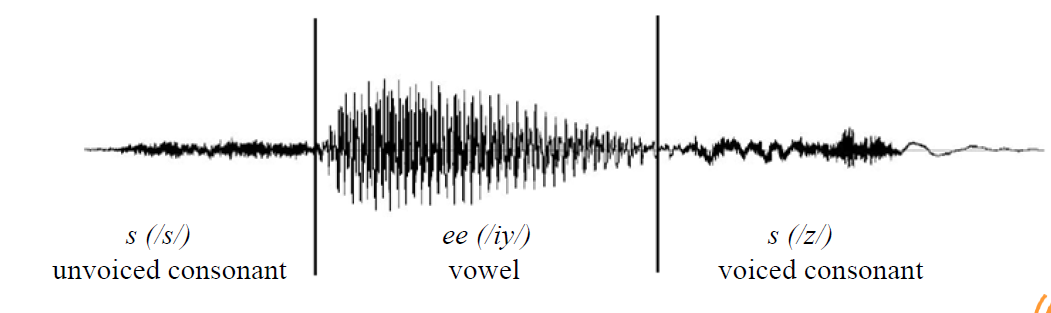
\includegraphics[scale=0.2]{Grafiken/bsp-sees.png}
	\end{itemize}
 		
\underline{Das Quelle-Filter-Modell} \\
	\begin{itemize}
		\item Wellengenerator: Periodische Schwingung der Stimmbänder
		\item Rauschgenerator: Luftstrom bei stimmlosen Phonen
		\item Systemmodell: Filtereigenschaft des Vokaltraktes (Mundraums)
		\item[] 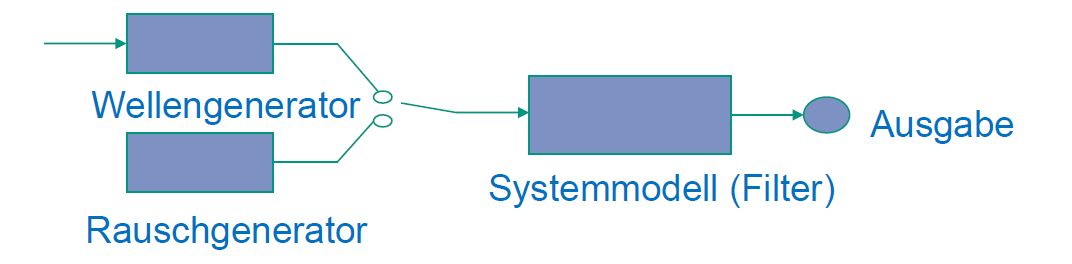
\includegraphics[scale=0.2]{Grafiken/quelle-filter-modell.png}
	\end{itemize}

\subsection{Akustische Phonetik und Phonologie}
\underline{Phonetik und Phonologie} \\
	\begin{itemize}
		\item Phonetik: Studium der Produktion, Klassifikation und Transkriptiopn von Sprachlauten -> Fokus liegt auf der akustischen Realisierung der Sprachlaute
		\item Phonologie: Studium der Verteilung und Struktur von Lauten in einer Sprache -> Hauptziel ist es, übergreifende Charakteristiken von Sprachlauten zu finden
	\end{itemize}

\underline{Phonetik} \\
	\begin{itemize}
		\item Artikulatorische Eigenschafen
			\begin{itemize}
				\item Laute können neben stimmhaft/stimmlos nach artikulatorischen Eigenschaften unterschieden werden
				\item Unterscheidung erfolgt entsprechend der Anatomie der wichtigen Artikulatoren und ihrer Position im Vokaltrakt
				\item Hauptkomponenten des menschl. Sprachproduk.apparats: Lungen, Trachea (Luftröhre), Pharynx (Rachen), Nasenhöhle und Mundhöhle. (Rachen + Mundhöhle = Vokaltrakt, Nasenhöhle = Nasaltrakt)
				\item Innerhalb des Vokaltrakts sind Stimmbänder, weicher Gaumen (Velum), harter Gaumen (Palatum), Zunge, Zähne und Lippen
			\end{itemize}
		\item Benennung von Sprachlauten
			\begin{itemize}
				\item Nasallaute:Luftstrom hauptsächlich durch Nase, gesenktes Velum (/n/)
				\item Orallaute: Luftstrom durch Mund, Velum verschließt Nasalraum
				\item Stoplaute (Plosive):Vokaltrakt kurzzeitig vollst. verschlossen (/p/, /b/)
				\item Frikative: Vokaltrakt teilw. verschlossen, Reibung entsteht (/f/)
				\item Approximanten: Vokaltrakt verengt, keine Reibung (/j/)
				\item Labial: Artikulationsort Lippen (/b/, /w/)
				\item Dental: Artikulation Zunge an Zähnen
				\item Alveolar: Alveole (Zahndamm) aktiv
				\item Palatal: Harter (vorderer) Gaumen aktiv
				\item Velar: Weicher (hinterer) Gaumen aktiv
				\item Glottal: Glottis, Stimmbänder aktiv (z.B. Be-amte)			
			\end{itemize}
		\item Konsonanten und Vokale
			\begin{itemize}
				\item Bei der Artikulation von Konsonanten befindet sich irgendwo im Vokaltrakt ein Hindernis (Stop, Verengung) für den Luftstrom
				\item Bei Vokalen liegt kein solches Hindernis vor
				\item Wichtige Eigenschaften für die Spracherkennung wichtig:
					\begin{itemize}
						\item Durschnittliche Dauer von Vokal ist viel länger als von Konsonant
						\item Vokale tragen den Hauptteil an Energie im Signal
						\item => Vokale wichtig für Spracherkennung, Konsonanten sind schwach und können mit Stille verwechselt werden
						\item Bei (englischem/deutschem) Text ist es gerade andersherum
					\end{itemize}
			\end{itemize}
		\item Modell des menschlichen Vokaltrakts
			\begin{itemize}
				\item Menschliche Vokaltrakt kann durch eine verlustfreie Röhre mit variablem Querschnitt approximiert werden
				\item Wichtige Approximation: Verkettung von endlichen vielen Röhren mit festen Querschnitt
				\item Mit dem Modell berechnen sich die Filereigenschaften des Vokaltrakts
				\item [] %G 12 - 18
			\end{itemize}
		\item Mathematische Beschreibung
			\begin{itemize}
				\item Unter geeigneten Bedingungen erfüllen Schallenwellen im Vokaltrakt die linearen partiellen DGLs
				\item "lossless tube"-Modell mit N Röhren approx. A
				\item analytische Lösung der DGLs möglich => Approximation der Frequenzantwort des Vokaltraktes
				\item Dieser Filter hat i.a. N konjugiert-komplexe Polstellen, die N/2 Resonanzfrequenzen (Formanten) entsprechen
				\item Tonhöhe der Formanten definieren den Laut
				\item Vokaltraktfilter kann durch ein nur-Pole-Modell, das nur Resonanzfrequenzen berücksichtigt, schon gut modelliert werden
			\end{itemize}
		\item Eigenschaften des Sprachspektrum
			\begin{itemize}
				\item Im Spektrum des Sprachsignals sind die Oberfrequenzen der Anregungsschwingung, die von den Stimmbändern kommt, besonders stark vertreten, so dass das Spektrum selber annährend periodisch ist
				\item Vokaltrakt wirkt als Filter auf die Anregung
			\end{itemize}
		\item Formanten
			\begin{itemize}
				\item Formanten lassen sich aus Spektrogrammen ablesen
				\item Die ersten beiden Formanten bestimmen im wesentlichen den Klang eines Vokals
			\end{itemize}
		\item Klassifikation von Vokalen: Formanten
			\begin{itemize}
				\item Das Vokaldreieck gibt an, welche Vokale im Mittel welche Formanten haben
				\item[] %G 12 - 23 rechts
			\end{itemize}
		\item Klassifikation von Vokalen: Formanten F1 und F2
			\begin{itemize}
				\item F1 entspricht der Hauptresonanzfrequenz des Rachenraumes
				\item F2 ist die Hauptresonanzfrequenz des Mundraumes
				\item Weg von Kehlkopf bis zur Zunge ist länger als Weg von Zunge bis Lippen => F1 < F2
				\item Zungenposition und Mundraum bestimmen die Werte F1 und F2
			\end{itemize}
		\item Diphtonge - Die charakteristischen Formanten F1 und F2 heißen auch formant targets, wenn
			\begin{itemize}
				\item Vokal ein spezifisches Ziel hat - Monophthong
				\item Zwei verschiedene Ziele kombinieren - Diphtonge
				\item Gibt einen fließenden Übergang zwischen den beiden Zielen
				\item Manche Sprachen (z.B. Mandarin) haben sogar Triphthonge 
				\item Diphtong wird i.d.R. genauso lang gesprochen wie ein Monophthong
			\end{itemize}
		\item Klassifikation von Konsonanten
			\begin{itemize}
				\item Werden durch Art und Ort der Artikulation beschrieben
				\item Artikulationsart - Mechanismus mit dem die Artikulation passiert
				\item Artikulationsort - Beschreibt Ort der Hauptverengung
				\item Sonorität (Schallfülle), Stimmhaftigkeit, Aspiration, Stärke
			\end{itemize}
		\item Vokaltraktformen: Plosive (Verschlusslaute)
			\begin{itemize}
				\item[] %G 12 - 28 + Spektogramm
				\item weiteres Plosiv: Glottal stop (Glottisschlag, Glottisverschlusslaut) - Luftstrom von den Stimmbändern im Kehlkopf gestoppt 
				\item Typisch: Kurzzeitig Luftstrom völlig unterbrochen
			\end{itemize}
		\item Vokaltraktformen: Nasale
			\begin{itemize}
				\item[] %G 12 - 13 +Spektogramm
				\item Mundraum komplett abgeschlossen und Rachenraum und Nasaltrakt miteinander verbunden
				\item Markante Eigenschaft: auffälligen fehlenden Frequenzbänder (gewisse Frequenzen im Mundraum werden vollständig reflektiert und so löschen sich Wellen aus)
			\end{itemize}
		\item Vokaltraktformen: Frikative (Reibelaute)
			\begin{itemize}
				\item[] %G 12 - 32 +Spektogramm
				\item Desweiteren gibt es glottalen Frikativ /h/ (wie in Haus) 
			\end{itemize}
		\item Phone und Phoneme
			\begin{itemize}
				\item Zwischen Schreibweise eines sprachl. Lautes und seiner Aussprache gibt es (prinzipiell) keinen Zusammenhang
				\item Phonetik: Sprachlaute haben keine inhärente Bedeutung
				\item Phonem: Kleinste Spracheinheit, die ein Wortpaar unterscheidet (minimales Paar) - Bsp: /kind/ != /rind/ -> /k/ und /r/ sind Phoneme
				\item Phon: Belieber Sprachlaut, der von anderen Sprachlauten akustisch unterschieden werden kann 
				\item Mit Phonem ist ein Bedeutungsunterschied verbunden und mit Phon nur ein akustischer Unterschied
				\item Schreibkonvention: /phonem/ vs [phon]
			\end{itemize}
		\item Phonetische Alphabete
			\begin{itemize}
				\item IPA: International Phonetic Alphabet (von der International Phonetic Association entwickelt + enthält Inventar für alle Laute aller Sprachen der Welt)
				\item Worldbet: 1-1 Abbildung von IPA-Symbolen auf ASCII-7 Symbole, um IPA-Alphabet auf Computern nutzbar zu machen
				\item Klein- und Großschreibung von Buchstaben hat auch Bedeutung
				\item Sampa: Basiert auch auf ASCII-7 Symbolen, wurde aber ursprünglich nur die deutsche und dann Indoeuropäische Sprachen entwickelt + Kürzlich auch auf weitere Sprachen ausgedehnt (X-Sampa)
			\end{itemize}
		\item IPA-Schema für Konsonanten + Vokale
			\begin{itemize}
				\item[] Konsonanten: %G 12 - 38
				\item[] Vokale: %G 12 - 39
			\end{itemize}
		\item Phone und Phoneme 
			\begin{itemize}
				\item Phoneme unterscheiden sich in Aussprachen durch:
					\begin{itemize}
						\item 1. Koartikulation, Kontext
						\item 2. Koartikulation bei variabler Sprechgeschwindigkeit
					\end{itemize}
				\item Wenn es mehrere Phone gibt, die dasselbe Phonem repräsentieren - heißt dann Allophone
			\end{itemize}
		\item Koartikulation
			\begin{itemize}
				\item Phoneme werden of auf systematische Weise von ihren Nachbarphonen beeinflusst
				\item Diesen Prozess bezeichnet man als Koartikulation
				\item In kontinuierlicher Sprache (mit variabler Sprechgeschwindigkeit)
					\begin{itemize}
						\item werden formant targets macnhmal nicht vollständig erreicht
						\item Betonungsmuster können verändert sein
						\item Laute können modifiziert werden (Assimilation)
						\item Laute können ganz verschwinden (Elision)
					\end{itemize}
				\item Effizientprinzip
					\begin{itemize}
						\item Sprecher versucht, den artikulatorischen Aufwand zu minimieren, ohne das dabei Information verlorengeht 
						\item Sprecher kann je nach Situation seinen Sprechgeschwindigkeit erhöhen 
					\end{itemize}
				\item Laute innerhalb einer Silbe beeinflussen sich mehr als benachbarte Laute in verschiedenen Silben
			\end{itemize}
		\item Prosodie 
			\begin{itemize}
				\item Eine Phrase kann, von der Intonation einzelner Laute abgesehen, auch als ganzes eine Melodie haben
				\item Eine Prosodie enthält Information über: Intention der Äußerung, Relevanz, Auflösung syntaktischen oder semantischen Zweideutigkeiten, Emotionen des Sprechers
				\item Prosodische Information ist: Intonation ("Melodie" des Satzes), Pausen, Betonung, Rhythmus
			\end{itemize}
	\end{itemize}

\subsection{Sprachperzeption}
\underline{Sprachproduktion und Sprachperzeption} \\
	\begin{itemize}
		\item Akustische Sprache pflanzt sich dann als Schalldruckwelle durch die Luft fort und wird vom menschlichen Ohr oder Mikrofon aufgefangen
	\end{itemize}
	
\underline{Sprachkommunikation von Mensch zu Mensch} \\
	\begin{itemize}
		\item[] %G 12 - 46
		\item A: Neurophysiologischer Prozess im Gehirn
		\item B: elek. Prozess in den efferenten Nervenbahnen
		\item C: Bewegung des Artikulationsapparates
		\item D: Erzeugung des akustischen Sprachsignals im Vokaltrakt
		\item E: Akustische Übertragung des Sprachsignals
		\item F: mechanischer Prozess im Mittelohr, hydromechanischer Prozess im Innenohr
		\item G: elek. Signale in den afferenten Nervenbahnen
		\item H: Neurophysiologischer Prozess im Gehirn des Empfängers
		\item I: Akustisches Feedback zum Ohr des Sprechers
	\end{itemize}
	
\underline{Physiologie des Ohres} \\
	\begin{itemize}
		\item Ohr empfängt die Schalldruckwellen aus der Luft
		\item Drucksignal wird in elek. Signal umgewandelt
		\item elek. Signal wird zum Gehirn weitergeleitet
		\item Außenohr:
			\begin{itemize}
				\item Ohrmuschen fängt durch ihre Form die Schallwelle ein und leitet sie in den Ohrkanal
				\item Orhkanal verstärkt das Signal
				\item Schließlich gelangt das Signal zum Mittelohr
				\item Signal Eingang + Ausgang: Schalldruckwelle in Luft
			\end{itemize}
		\item Mittelohr: 
			\begin{itemize}
				\item Schalldruckwellen bewegen das Trommelfell
				\item Dadurch gerät die Knochenstruktur (Hammer, Amboss, Steigbügel) in Schwingung 
				\item Durch das ovale Fenster wird eine Druckwelle der Flüssigkeit des Innenohres erzeugt
				\item Signal Eingang: Schalldruckwelle in Luft
				\item Signal Ausgang: Schalldruckwelle in Flüssigkeit
				\item Schalldruckwiderstand: Luft (niedrig), Flüssigkeit (hoch)
				\item Mittelohr übersetzt die Schallwelle von niedrigem Widerstand zu hohem Widerstand
				\item Knochenstruktur zwischen dem großen Trommelfell und dem kleinen ovalen Fenster dient als Verstärker
			\end{itemize}
		\item Innenohr:
			\begin{itemize}
				\item Die Cochlea ist eine spiralenförmige Röhre 
				\item Cochlea ist mit den Cochlea Filtern besetzt 
				\item Filter übersetzen die Wellen in Nervensignale
				\item Signal Eingang: Schalldruckwelle in Flüssigkeit
				\item Signal Ausgang: Elektrisches Signal im Gehörnerv
			\end{itemize}
		\item Cochlea:
			\begin{itemize}
				\item Cochlea Filter schwingen in den Wellen
				\item Filter sind mit der Basilarmembran verbunden
				\item Bewegung erzeugt eine Anregung in der Basilarmembran
				\item Dieses Signal wird dann durch den Gehörnerv an das Gehirn weitergeleitet
			\end{itemize}
	\end{itemize}

\underline{Wahrnehmung verschiedener Frequenzen} \\
	\begin{itemize}
		\item An verschiedenen Punkten entlang der Cochlea reagiert die Basilarmembran auf unterschiedliche Frequenzen
		\item Das Gehör basiert auf Frequenzen
	\end{itemize}

\underline{Physikalische vs. perzeptuelle Eigenschafen} \\
Gibt grundlegenden Unterschied zwischen der Wahrnehmung (Perzeption) eines Lautes und seinen messbaren physikalischen Eigenschaften. Manche physikalischen und perzeptuellen Eigenschaften hängen miteinander zusammen, sind aber keineswegs identisch
%G 12 - 55
	\begin{itemize}
		\item Unterschied: frequenzabhängige Wahrnehmung der Lautstärke (Empfindlichkeit variiert mit der Frequenz, Lautstärke != Intensität)
		\item Wahrnehmung hängt abvon: Resonanzfreq. des Gehörgangs, Übertragungsfunktion der Gehörknöchelchen
	\end{itemize}
	
\section{Sprackerkennung - Algorithmik}
\subsection{Sprachsignalverarbeitung}
Wir benötigen eine Repräsentation jedes Frames, die das enthaltene Sprachsegment möglichst gut charakterisiert
	\begin{itemize}
		\item Geringer Aufwand in Speicherplatz und Rechenzeit
		\item Verschiedene Phoneme sollen gut unterscheidbar sein
		\item Robust gegenüber Störungen 
	\end{itemize}

\underline{Speech Coding} \\
Wie repräsentiert man Sprache in digitaler Form?
	\begin{itemize}
		\item Direkte Speicherung der Wellenform (beachte Effekte von Sampling/Quantisierung, akustische Signal sollte zurückzugewinnen sein)
		\item Parametrische Repräsentation (gewisse Eigenschaften des Sprachsignals werden bezogen auf ein gewisses Modell gespeichert)
	\end{itemize}

Wie beurteilt man die Qualität einer Sprachcodierung?
	\begin{itemize}
		\item Qualität vs. Bitrate
		\item Benötigte Rechenleistung (Echtzeitanforderungen)
		\item Quantisierungsrauschen
		\item Robustheit bei weiteren Verarbeitungsschritten
		\item Fehlertoleranz
		\item Verhalten bei nichtsprachlichen Signalen
		\item Hohe Verständlichkeit für Menschen
	\end{itemize}
	
\underline{Sampling} \\
	\begin{itemize}
		\item Erster Schritt: A/D-Wandlung
		\item Hörbereich: ca. 200 Hz - 20 kHz
		\item Sprachsignal: ca. 300 Hz - 8 kHz
		\item Nach Nyquist-Theorem tasten wir in der Regel mit min. 16 kHz ab
		\item weniger problematisch ist die Quantisierung (16-bit-Quantisierung ist ausreichend für Spracherkennung)
	\end{itemize}
	
\underline{Mel-Frequency Cepstral Coefficients (MFCC)} \\
\underline{Framing (Fensterung} \\
Bei Framing gibt es 3 Dinge zu beachten:
	\begin{itemize}
		\item Frame Shift (die Schrittweite zwischen Frames)
		\item Frame Size (Fenstergröße)
		\item Fensterform
	\end{itemize}

Schrittweite ergibt sich aus Spracherzeugung und -perzeption:
	\begin{itemize}
		\item Sprechrate: 10-30 Phone/s => Phonem hat eine Länge von ca. 30 -100ms
		\item Jedes Phon kann aus mehreren Segmenten bestehen, üblicherweise wird es durch drei Zustände (Anfang, Mitte, Ende) modelliert
		\item Kleinstes Segment entspricht daher 10ms => Frame Shift ist deshalb 10ms
	\end{itemize}
	
\underline{Das Hamming-Fenster} \\
	\begin{itemize}
		\item Standardfenster in der Sprachsignalverarbeitung
		\item[] %G 13 - 12
		\item Fenstergröße beträgt etwa 1.5-2-fache des Frameshifts
		\item Typische Fenstergröße: ca. 16ms
	\end{itemize}
	
\underline{Fouriertransformation} \\
	\begin{itemize}
		\item Nächster Schritt zur Berechnung von MFCCs ist Frequenzanalyse der einzelnen Frames
		\item Zur Erinnerung: STFT
		\item[] %G Formel 12 - 15
		\item w[n] ist die Hamming-Fensterfunktion
		\item Die STFT erzeugt N Frequenzsamples aus N Zeitsamples - 1 komplexe Zahl pro Frequenz, Symmetrisch im Betrag + antisymmetrisch in der PHase => reicht die positiven Frequenzen zu betrachten
		\item Effiziente Berechnung: FFT (Fast Fourier Transform)
		\item Menschl. Ohr ist sehr empfindlich für die Phase des Audiosignals (aber nicht in 10-20ms Fenstern), daher reicht es in den Fenstern dieser Gröe das Amplitudenspektrum (Betrag des Spektrums) zu betrachten
	\end{itemize}
	
\underline{Mel-Filterbank} \\
	\begin{itemize}
		\item Betrachten wir uns die DTFT auf einem 16 kHz gesampelten Sprachframe, liefert -> 16ms entsprechen 256 Samples, gibt es 256 Frequenzkomponenten im Bereich von -8 kHz bis 8 kHz (aus Symmetriegründen sind 128 von ihnen interessant für uns)
		\item Problem: Diese Auflösung im Frequenzbereich ist viel zu hoch
		\item Es wäre besser, größere Frequenzbereiche zu betrachen
		\item Lösung: Vor der Logarithmierung verwenden wir eine Filterbank
		\item Filterbank fasst jeweils benachbarte Frequenzen gewichtet zusammen
		\item Filterbank orientiert sich am menschlichen Gehör (lin. Frequenzantwort zwischen 0 Hz und 1000 Hz, log. Antwort über 1000 Hz)
		\item Meistens benutzt: Mel-Filterbank (40 überlappende Dreiecksfilter zwischen 300 Hz und 8000 Hz + Verringert Dimensionalität des Signals auf 40 Koeffizienten pro Frame
	\end{itemize}
	
\underline{Cepstrum} \\
 	\begin{itemize}
 		\item Zunächst berechnen wir den Logarithmus des Amplitudenstpektrums (menschl. Gehör unterscheidet Frequenzen auch logarithmisch)
 		\item $e(t) * h(t) \rightarrow E(z) \cdot H(z) \rightarrow log E + log H$
 		\item Frequenzanalyse des logarithmierten Spektrums ergibt das Cepstrum
 		\item Einheit des Cepstrums ist die Quefrenz (auch Hz)
 		\item Cepstrum ist die Summe vom Einfluss der Anregungsschwingung und dem Einfluss vom Vokaltrakt (weil die FT linear ist)
 		\item Anregungsschwingung von 200 Hz im Beispiel sichtbar
 		\item[] %G 13 - 23
 	\end{itemize}
 	
\underline{Log-Mel-Spektrogramm} \\
	\begin{itemize}
		\item Mel-Filterbank behält die grobe Struktur des ursprünglichen Spektrogramm
		\item Durch anschließende Logarithmierung und inverser FT, erhält man die Mel-Frequency Cepstral Coefficients (MFCC)
		\item Überlicherwise werden die ersten 13-14 MFCCs verwendet
	\end{itemize}	
	
%G 13 - 25 		

\underline{Dynamik des Sprachsignals} \\
	\begin{itemize}
		\item Typischerweise werden etwa 14 Koeffizienten pro Frame extrahiert
		\item Nicht nur Betrag eines Koeffizienten ist interessant, sondern auch Änderungsrate (1. Ableitung) und "Beschleunigung" (2. Ableitung)
		\item Diese kann man wie folgt approximieren:
			\begin{itemize}
				\item Differenz zwischen Frames t und t-1 $\rightarrow$ "delta"-Koeffizienten, 1. Ableitung
				\item Differenz der deltas $\rightarrow$ "delta-delta"-Koeffizienten, 2. Ableitung 
				\item Alternativ kann man benachbarte Frames zeitverschoben "stacken"
			\end{itemize}
	\end{itemize}
	
\subsection{The Big Picture/Fundamentalformel der Spracherkennung}

\underline{Fundamentalformel der Spracherkennung} \\
	\begin{itemize}
		\item Gegeben eine Sequenz von Merkmalsvektoren X, finde wahrscheinlichste Wortsequenz W
		\item[] %G 13-32
	\end{itemize}
	
\underline{Automatic Speech Recognition} \\
	%G 13-34 
	\begin{itemize}
		\item Aussprache-Wörterbuch 
			\begin{itemize}
				\item Die Verbindung zwischen der Akustik und der geschriebenen Sprache (Beschreibe ein Wort als Konkatenation von Phonemen)
				\item[] %G 13-35
			\end{itemize}
		\item Akustisches Modell
			\begin{itemize}
				\item $p(X|W)$
				\item Gegeben W, mit welcher Warhscheinlichkeit wird die Merkmalssequenz X beobachtet?
			\end{itemize}
	\end{itemize}

\underline{Sprachproduktion als stochastischer Prozess} \\
	\begin{itemize}
		\item Das gleiche Wort/Phonem/Laut hört sich jedesmal anders an
			\begin{itemize}
				\item betrachte Wörter/Phoneme/Sprachteile als Zustände eines Sprachproduktionsprozesses
				\item diese Zustände haben unterschiedliche akustische Realisierungen
				\item wir können nur die Realisierung beobachten, nicht den Zustand
			\end{itemize}
		\item In einem Zustand können verschiedene Laute beobachtet werden, aber nicht alle Laute sind in jedem Zustand wahrscheinlich (in einem gegebenen Zustand emittiert der Sprachprozess einen Laut entsprechend einer bestimmten Wahrscheinlichkeitsverteilung/-dichte
		\item Produktionsprozess kann Übergänge aus einem Zustand in einen anderen machen, aber nicht alle Übergänge sind wahrscheinlich (Auch Zustandsübergänge folgen einer Wahrscheinlichkeitsverteilung)
	\end{itemize}
	
\underline{HMMs in der Spracherkennung} \\
	\begin{itemize}
		\item Ein typisches HMM (für das Wort "can")
		\item[] %G 13-39 
		\item 3-Zustands-Bakis-Modell pro Phonem
		\item Self-Loops erlauben beliebige Dauer eines Phonems
		\item Jeder Zustand modelliert Teil eines Phonems (Anfang, Mitte, Ende)
		\item Diesen Teil eines Phonems nennt man auch Subphonem
		\item Zustände, die zum selben "akustischen Phänomen" gehören, teilen sich ein Modell $Model S_1 = Model S_7 = Model g-b$ 
		\item[] %G 13-40
		\item Vorteile: Bessere Ausnutzung der Trainingsdaten, höhere Robustheit, bessere Parameterabschätzung, Rechenzeit wird gespart
	\end{itemize}

\underline{HMM-Training} \\
 	\begin{itemize}
 		\item 1. Init:	
 			\begin{itemize}
 				\item HMM muss initialisiert werden, vor dem eigentlich Training
 				\item Init alle Parameter zufällig oder identisch
 				\item Verwende gelabelte Daten (durch anderen Erkenner, manuell) - Init Gaussverteilungen z.B. mit K-Means o.ä.
 			\end{itemize}
		\item 2. Training / Iterative Optimierung 
			\begin{itemize}
				\item 1. Berechne Zustandsordnung (Forward-Backward, Viterbi)
				\item 2. Schätze HMM-Parameter neu (Baum-Welch, EM)
				\item Abbruchkriterien: keine Verbesserung der Scores (log-likelihoods) mehr auf Trainingsmenge oder separater Kreuzvalidierungsmenge, feste Anzahl Iterationen
			\end{itemize}
 	\end{itemize}
 	
\underline{Kontextabhängige Modellierung} \\
	\begin{itemize}
		\item Betrachte die Aussprachen von true, train, table und tell
		\item[] %G 13-42
		\item Die wahre Aussprache ist aber eher wie folgt
		\item[] %G 13-42
		\item Phonem T wird abhängig vom Kontext unterschiedlich ausgesprochen
		\item Erste Idee
			\begin{itemize}
				\item Eigentliche Aussprachen anstelle der Phoneme verwenden: /ch/ /r/ /uw/ statt /t/ /r/ /uw/
				\item Problem: /ch/ in true klingt anders als /ch/ in church
			\end{itemize}
		\item Zweite Idee
			\begin{itemize}
				\item Kontextabhängige Einheiten
				\item[] %G 13-43
			\end{itemize}
		\item[] $\rightarrow$ Trainiere unterschiedliche HMMs abhängig vom phonetischen Kontext
		\item Ein Phonem was von Vorgänger und Nachfolger abhängt ist ein Triphon
		\item Was passiert, wenn wir einheitlich jedes Phonem als Triphon modellieren? 
			\begin{itemize}
				\item Manche Kontexte kommen sehr selten vor (zu wenig Trainingsdaten!)
				\item Manche Kontexte kommen vielleicht im Trainingsmaterial gar nicht vor, aber könntne beim Decoding benötigt werden?
			\end{itemize}
		\item Ansatz: Fasse bestimmte Phoneme zu Klassen zusammen (Wissensbasiert: Artikulatorische Feature (Frikative, Vokale, etc. ))
		\item Triphone abhängig von diesen Klassen anstelle von einzelnen Phonemen
	\end{itemize}

\underline{CART} \\
	\begin{itemize}
		\item Verwende datengetriebene Methode, um Kontextklassen zu bilden
		\item CART steht für Classification und Regression Tree
		\item Aufteilung erfolgt durch binäre Fragen und deren Informationsgewinn
		\item Vorgehensweise
			\begin{itemize}
				\item Initial gibt es so viele Blätter im Baum wie Phoneme (Jedes Blatt enthält ein kontextunabhängiges Phonem)
				\item Iteratives vorgehen:
				\item 1. Bestimme Informationsgewinn jeder möglichen Frage für jedes Blatt im Baum
				\item 2. Spalte Blatt mit der Frage mit höchstem Informationsgewinn auf
			\end{itemize}
		\item Abbruchkriterien
			\begin{itemize}
				\item Maximale Anzahl Blätter
				\item Minimaler Informationsgewinn
				\item Minimale Menge an Trainingsdaten in jedem Blatt
			\end{itemize}
		\item[] %G  13-45
	\end{itemize}

\underline{Sprachmodellierung} \\
Was brauchen wir noch, um natürliche menschliche Sprache gut erkennen zu können?
	\begin{itemize}
		\item Lexikalisches Wissen: Vokabular, Aussprachewörterbuch
		\item Akustische Klassifikation haben wir gelernt: HMMs
		\item Wissen über die Sprache ist ebenso wichtig
			\begin{itemize}
				\item Ist eine Wortsequenz grammatikalisch korrekt (schwierig!)
				\item Hat eine Wortsequenz eine sinnvolle Bedeutung?
				\item Welche Worte sind jetzt wahrscheinlich?
				\item Wie kann man den Ablauf eines Dialogs verfolgen?
			\end{itemize}			 
	\end{itemize}
	
\underline{Stochastische Sprachmodelle} \\
	\begin{itemize}
		\item Modellieren Abfolge von Worten und Sätzen
		\item Gegebene Wortfolge W wird eine gewisse Auftrittswahrscheinlichkeit P(W) haben
		\item Sprachmodellierung ist in der Spracherkennung essentiell
			\begin{itemize}
				\item Weitere Informationsquelle beim Erkennungsprozess
				\item Hilft bei Unterscheidung von Homophonen
				\item Verringert den Suchraum 
				\item Erster Schritt zur semantischen Analyse
			\end{itemize}
		\item Schwierigkeit 1: Welche Wortsequenzen sind in gesprochener Sprache möglich?
			\begin{itemize}
				\item Klassische Methode zur Beschreibung: Formale Grammatik
				\item Aber wie beschreibt man die volle Flexibilität der deutschen Sprache?
			\end{itemize}
		\item[] $\rightarrow$ Wir brauchen eine probabilistische Methode, die ausdrucksstark, einfach aufzusetzen, und möglichst fehlertolerant ist
		\item Schwierigkeit 2: Anzahl möglicher Wortfolgen W wird sehr schnell sehr groß, wenn man die maximale Länge der Wortfolgen wachsen lässt
		\item $\rightarrow$ Brauchen eine effiziete Approximation von Sprachmodellwahrscheinlichkeiten (und einen guten Algorithmus)
	\end{itemize}
	
\underline{Wahrscheinlichkeit einer Wortsequenz} \\
	\begin{itemize}
		\item Wahrscheinlichkeit einer Wortsequenz P(W) kann zerlegt werden $P(W) = P(w_1 w_2 .. w_n) = P(w_1) \cdot P(w_2 | w_1) \cdot ... P(w_n | w_1 w_2 ... w_{n-1})$
		\item Wahrscheinlichkeit von $w_n$ hängt von allen Worten $w_1 w_2 ... w_{n-1}$ ab
		\item Vorberechnung aller Wahrscheinlichkeiten aller Wortfolgen unmöglich
		\item Mögliche Lösungen:
			\begin{itemize}
				\item $P(W|history)$ "on the fly" berechnen (selten, sehr teuer)
				\item Äquivalenzklassen von Historien bilden, um deren Anzahl zu reduzieren
			\end{itemize}
		\item Grammatik nur bei kleinen Vokabularen und beschränkter Domäne sinnvoll (z.B. Telefonservice)
	\end{itemize}

\underline{Sprachmodelle} \\
Verschiedene Methoden, Historien in Äquivalenzklassen einzuteilen
	\begin{itemize}
		\item Grammatische Eigenschaften
		\item POS (Part of Speech)
		\item Semantische Bedeutung der vorherigen Wörter
		\item Kontextgleichheit 
		\item Automatisches Clustering nach bestimmten Regeln
		\item Historie auf eine gewisse Anzahl Wörter beschränken (Unigramm, Bigramm, Trigramm)
	\end{itemize}

\underline{n-Gramm-Sprachmodelle} \\
Der übliche Ansatz, n-Gramm-Wahrscheinlichkeiten abzuschätzen:
	\begin{itemize}
		\item Suche Domänen spezifische Texte (Transkriptionen der Audiodaten des Trainings, Suche im Netz)
		\item bestimme Häufigkeit, mit der das Wort w nach einer Historie h auftritt
		\item zähle die Häufigkeit der Historie h im gesamten Text und normalisiere $P(w|h) = \frac{count(h,w)}{count(h)}$
	\end{itemize}
	
\underline{Automatic Speech Recognition - Suche} \\
	\begin{itemize}
		\item Suche: Akustik, Aussprachen und Sprache verbinden + gesprochene Sprache erkennen
		\item Um eine Sprachäußerung zu erkennen müssen alle möglichen Wortfolgen miteinander verglichen weren
		\item Die Gesamtheit aller möglichen Musterfolgen heißt Suchraum
		\item Typischer Suchraum hat extrem viele Elemente
		\item[] $\rightarrow$ Auswertung aller Wortsequenzen nicht möglich
		\item Benötigen Algorithmus der den Suchraum nur teilweise prüft und möglichst gute Hypothese findet 
		\item Dieses Problem nennt man Suche oder Decoding 
	\end{itemize}

\underline{Tiefensuche und Breitensuche} \\
	\begin{itemize}
		\item Tiefensuche
			\begin{itemize}
				\item Zu jedem Zeitpunkt wird nur der Pfad mit der höchsten Wahrscheinlichkeit weiterverfolgt (A* Suche) und Pfade werden zeitasynchron expandiert
				\item Vorteil: Suche findet für das gegebene Modell das optimale Ergebnis
				\item Nachteile: Unter Umständen müssen sehr viele Pfade expandiert werden + schlecht zu parallelisieren
			\end{itemize}
		\item Breitensuche (Standard-Suchmethode in der Spracherkennung)
			\begin{itemize}
				\item Expandiere die Pfade zeitsynchron und für jeden Frame werden nur eine feste/variable Anzahl an Pfaden weiterverfolgt (beam search)
				\item Vorteile: kann verschiedene Wissensquellen zeitsynchron kombinieren + gut parallelisierbar
				\item Nachteil: nicht garantiert, die optimale Lösung des Suchproblems zu finden
			\end{itemize}
	\end{itemize}
 

\section{Muskelaktivität - Einstehung, Messung (EMG), Anwendungen}
\subsection{Einstieg}

\begin{itemize}
	\item Ziel: Erfassung der menschlichen Bewegeung 
	\item Bewegungserfassung durch: visuelle Erfassung durch Kameras, direkte Erfassung der Bewegung, indirekt durch die Erfassung der Muskelaktivität die die Bewegung erzeugt
	\item Elektromyographie (EMG): Erfassung der elektrischen Potentiale, die durch Muskelaktivität entstehen
	\item Mensch-Maschinen-Schnittstelle: Erfassung von willentlichen Bewegungen
	\item Beschränkung auf die Betrachtung des Signals ab dem Rückenmark ($\alpha$-Motoneuronen)
\end{itemize}

\underline{Menschliche Bewegung} \\
Definition: Bewegungen sind räumliche Verschiebungen von Gewebe
	\begin{itemize}
		\item Größräumige Bewegungen z.b. Bewegungen der Beine beim Gehen
		\item Kleinste, fast unmerkliche Bewegungen z.B. Mimik
		\item Jegliche Bewegung geschieht durch Muskeln
			\begin{itemize}
				\item Quergestreifte Muskeln: Skelettmuskeln (Muskeln des Bewegungsapparates), Herzmuskel (unwillkürlich gesteuert)
				\item Glatte Muskeln: Muskeln der inneren Organe und Gefäße
				\item Augenmerk gilt den Skelettmuskeln
			\end{itemize}
	\end{itemize}

\subsection{Aufbau des Muskels}
	\begin{itemize}
		\item Bewegung und Muskelarbeit entsteht durch Muskelverkürzng (Muskelkontraktion)
		\item Elemente, die zur Kontraktion fähig sind, heißen Myofibrillen
		\item Skelettmuskeln sind über Sehnen mit dem Skelett (Knochen) verbunden
		\item Kleinste funktionelle Einheit des Skelettmuskels ist die Muskelzelle = Muskelfaserzelle = Muskelfaser 
		\item Muskelfasern schließen sich zu Faserbündeln zusammen, die man mit bloßem Auge als "Fleischfasern" erkennen kann
		\item Muskelfaser: 1/100 - 1/10 mm Durchmesser, Bis 20cm Länge
		\item Zytoplasma (Zellplasma) der Muskelfaser (Sarkoplasma) wird von der Membran (Sarkolmm) umschlossen
		\item Im Inneren der Muskelfaser befinden sich die Myofibrillen
		\item Nehmen größten Teil des Zellvolumens ein
		\item Myofibrillen: langestreckt, Durchmesser ca. 1 $\mu m$
		\item Myofibrillen sind in Zonen unterteilt
		\item Diese Zonen weiter unterteil in A-Bande (stark brechend) und I-Bande (schwach brechend)
		\item Innerhalb der I-Bande befindet sich die Z-Linie
		\item Bereich zwischen zwei Z-Linien: Sarkomer
		\item Unter dem Mirkoskop A/I-Bande als Querstreifen erkennbar - deshalb "quergestreifte Muskulatur"
		\item Myofibrillen bestehen aus 2 Typen von parallel gelagerten fadenartigen Filamenten: Myosinfilamente (langgestreckte Myosinmoleküle - Protein), Aktinfilamente (kugelförmiges Protein, kettenförmig gelagert verdrillt zu Faden)
		\item Beide Filamenttypen berühren sich, wo Ausstülpungen des Myosinmoleküls, die Myosinköpfe, das Aktinfilament berühren
		\item[] %G 14- 14 links unten
		
	\end{itemize}
%G Muskel aufbau

\subsection{Muskelkontraktion}
\begin{itemize}
	\item Folgender Vorgang läuft bei Muskelkontraktion ab:
		\begin{itemize}
			\item Aktivierung Myosin-Aktin-Querbrücke
			\item Verschiebung der Aktin- und Myosinfilamente in Längsrichtung gegeneinander (Filamentgleitmechanismus)
		\end{itemize}
	\item Sind minimale Verschiebungen, aber in vielen hintereinander Sarkomeren
	\item Insgesamt ergibt sich so eine beachtliche Längenverkürzung
	\item $\rightarrow$ Prozess nennt man Muskelkontraktion
\end{itemize}

Ausgangssituation:
	\begin{itemize}
		\item Muskeln in erschlafftem Zustand
		\item ATP (Adenosintriphosphat) gespalten in ADP + P und an Myosinkopf gebunden
		\item Bindungsstellen des Aktins mit Tropomyosin belegt
	\end{itemize}

Vorgang bei Erregung:
	\begin{itemize}
		\item Muskelfaser wird erregt, dadurch strömt $Ca^{2+}$ in die Muskelfibrillen
		\item Diese Depolarisierung breitet sich als Aktionspotential aus
		\item $Ca^{2+}$-Ionen binden sich an Troponinmoleküle $\rightarrow$ Tropomysin löst sich von Aktin-Bindungsstellen $\rightarrow$ Myosin kann an Aktin andocken
		\item ADP und P wurden freigesetzt $\rightarrow$ Myosinhals knickt um
		\item Myosinfilament zieht sich an Aktin entlang
		\item Muskel kontrahiert
	\end{itemize}

Nach der Kontraktion:
	\begin{itemize}
		\item ATP bindet sich an Myosinköpfchen
		\item ATP wird aufgespalten
		\item Durch Energie die bei der Spaltung in ADP + P frei wird, klappt Myosinkopf zurück in Ausgangsposition und löst sich von Bindungsstelle
	\end{itemize}
	
\underline{Neuromuskuläre Übertragung} \\
Woher kommt Erregung eines Muskels, die eine Kontraktion bewirkt?
	\begin{itemize}
		\item Aktivierung einer quergestreiften Muskelfaser erfolgt durch ein Motoneuron
		\item Spinale Motoneuronen = $\alpha$-Motoneuronen
		\item Axon des $\alpha$-Motoneuronen bildet Bündel mit anderen Axonen einen efferenten Nerv, der vom Rückenmark zur Peripherie läuft
		\item Axon endet in einer oder mehreren Synapsen, die an Muskel andocken - heißen motorische Endplatten
	\end{itemize}
	
\underline{Aktivierung einer Muskelfaser} \\
	\begin{itemize}
		\item Wenn das Motoneuron feuert, ensteht im Muskel ein Aktionspotential (MUAP)
		\item breitet sich längs der Muskelfaser vom Ursprung aus
		\item Führt zu Kalziumeinstrom
		\item Dieser führt zur Konformationsänderung der Myosinköpfe und somit zur Muskelkontraktion
		\item Zahl der von einem Motoneuron versorten Muskelfasern liegt zwischen 1 und mehreren Tausen
		\item Jede Muskelfaser hat nur eine Motorische Endplatte (d.h. wird von genau einem Motoneuron innerviert)
		\item Motorische Einheit (MU) = ein Motoneuron + alle von ihm innervierten Muskelfasern
		\item Um Muskelkontraktion aufrecht zu erhalten muss das Motoneuron wiederholt feuern, Abfolge von Aktionspotentialen (MUAPT)
		\item Intervalle zwischen den einzelnen MUAPs und MUAPT sind etwa gaussverteilt
	\end{itemize}
	
\underline{Kontraktionsstärke} \\
Die Stärke der Kontraktion hängt von Zahl der den Muskel versorgenden gleichzeitig feuernden Motoneuronen und von der Frequenz ihres Feuerns ab

\subsection{Elektromyographie (EMG)}
Elektromyograpie: Das Studium der Muskelfunktion durch Erforschung des elek. Signals, das die Muskeln erzeugen

\underline{Aktionspotentiale} \\
	\begin{itemize}
		\item Reizung der Muskelzelle erzeugt Aktionspotential in der Muskelfaser (MUAP)
		\item Aktionspotential entsteht durch Einstrom von Ionen in dne Muskel
		\item Durch das Aktionspotential entstehenden Potentialdifferenzen - invasiv und an der Hautoberfläche messbar
		\item Besonders an der Hautoberfläche: Überlagerung vieler Aktionspotentiale, Identifizierung einzelner Potentialquellen ist schwierige Aufgabe
		\item Betrachtung eines einzelnen Aktionspotentials an der Hautoberfläche: Plaziert man zwei Elektroden an zwei Positionen A (links) und B (rechts) auf dem Muskel (bipolare Ableitung)
			\begin{itemize}
				\item 1. Muskel in Ruhe: überall Ruhepotential, keine Differenz zwischen A und B
				\item 2. Muskel wird aktiviert, d.h. Aktionspotential AP entsteht
				\item 3. Da AP sich nur längs der Muskelfasern ausbreitet, wird die Elektrode nahe der Quelle A schneller von der Depolarisation erfasst als die quellferne Elektrode B $\rightarrow$ Potentialdifferenz A-B > 0
				\item 4. AP wandert weiter und erreicht nun Elektrode B $\rightarrow$ nun ist A-B < 0
				\item 5. AP wandert noch weiter, Potentialdifferenz ist wieder 0
			\end{itemize}
	\end{itemize}

\underline{EMG-Signal} \\
	\begin{itemize}
		\item Bei längerer Muskelkontraktion entsteht eine ganze Serie von Aktionspotentialen: MUAPT
		\item Unterschiede zwischen Signale durch Oberflächen- und Nadelelektrode: Oberflächen-EMG hat viel mehr Rauschen, Formen der einzelnen MUAPs eher schlecht erkennbar - erscheint tiefpassgefiltert
	\end{itemize}
	
\underline{Messung - Nadel- vs Oberflächenelektrode} \\
	\begin{itemize}
		\item Nadelelektrode: wird direkt in Muskel eingebracht
			\begin{itemize}
				\item Vorteile: spezifische + eng umrissene Aufzeichnungszone, erfasst auch kleine und tiefliegende Muskeln
				\item Nachteile: sind invasiv und erfordern sterile Bedingungen (nur durch Arzt einzubrinen), schwierig extakte Position wiederholt zu treffen
			\end{itemize}
		\item Oberflächenelektrode: 
			\begin{itemize}
				\item Vorteil: keine Schmerzen, Risiko
				\item Nachteil: Mehr Cross-Talk, schlechtere räumliche Auflösung
			\end{itemize}
		\item Nur Oberflächenelektroden im Bereich der Benutzerschnittstellen
	\end{itemize}
	
\underline{Muskel als Leiter} \\
	\begin{itemize}
		\item Relativ schlechter elek. Leiter
		\item Muskel wird als Tiefpassfilter
		\item Leitfähigkeit in Richtung der Muskelfasern höher als senkrecht zu ihnen
		\item Daten abgeleiterer Potentiale stark von der Elektrodenpositionierung abhängig
		\item Elektrodenabstand von der aktiven Faser spielt entscheidene Rolle
	\end{itemize}
	
\subsection{Anwedungsbeispiele}

\underline{Klinische Anwendung} \\
	\begin{itemize}
		\item Verhalten des Muskels bei gewissen wohldefinierten Reizen zu untersuchen
		\item exakt quantifizierbare Eigenschaften des Signals zu untersuchen
		\item nach Möglichkeit Verwendung von Nadelelektroden
		\item Erster Schritt von EMG in med./physio. Anwendungen ist oft Zerlegung des Signals in einzelne MUAPTs
		\item Algorithmus zur Zerlegung eines EMG-Signals:
			\begin{itemize}
				\item 1. Suche nach nächstem Peak im Rohsignal - dieser wird Knadidat für MUAP
				\item 2. Ordne diesen Peak einer Klasse von MUAPs zu bzw. erzeuge neue Klasse. Bei Bedarf kann ein menschlicher Experte eingreifen.
				\item 3. Nach erfolgreicher Zuordnung wird der Peak vom Rohsignal subtrahiert, Restsignal wird dann mit Schritt 1 weiterverarbeitet
			\end{itemize}
		\item Algorithmus bricht ab, wenn im Restsignal keine Peaks mehr vorhanden sind
		\item Algorithmus wird seit ca. 30 Jahren so verwendet
	\end{itemize}
	
\underline{Sonstige Anwedungen} \\
	\begin{itemize}
		\item Emotionserkennung
			\begin{itemize}
				\item Erkennung von Gesichtsausdrücken mittels EMG
				\item Warum? Nicht-invasive Methode, kleines Device, Elektroden einfach anzubringen
				\item Warum keine Videoerkennung? EMG in der Lage, Bewegungen aufzunehmen die auf Videos nicht sichbar sind + Mobiler kabelloser Rekorder kann überall mit hingenommen werden + benutzte Elektroden sind klein und leicht (nicht störend)
				\item Elektroden werden auf Muskeln plaziert, die an Gesichtsausdruck beteiligt sind
			\end{itemize}
		\item Erkennung von Fingerbewegungen
			\begin{itemize}
				\item Fingermuskulatur befindet sich am Unterarm
				\item Erlaubt Erfassung ohne Sensorik an der Hand
				\item Signale liefern auch Information über Kraft
				\item Problem: Crosstalk
			\end{itemize}
		\item EMG Prothesensteuerung/EMG-basierte Exoskelette
		\item FES- Funktionelle Elektrostimulation
			\begin{itemize}
				\item Verfahren zur Wiederherstellung der Bewegungsfunktion der Gliedmaßen
				\item Anwendungsgebiet: Lähmungen, bei denen nur Nervenbahnen zum betreffenden Muskel, aber nicht der Muskel selbst geschädigt ist
				\item Ziele: 1. Verhinderung von Muskelschwund und Sehnenkontraktion, 2. Steuerung des betreffenden Muskels
				\item Elektroden werden am Muskel angebracht (Oberflächenelektrode oder Implantat) $\rightarrow$ Übertragen elektrische Impulse an Muskel $\rightarrow$ Muskel kontrahiert
				\item Sensoren an gesunde Körperteilen anbringen 
				\item Erfassen der Bewegung $\rightarrow$ Übertragung auf defekten Muskel
			\end{itemize}
	\end{itemize}
 		
 		
\section{Elektrodermale Aktivität}
\subsection{EDA (ElektroDermale Aktivität}

\underline{Definition Elektrodermale Aktivität} \\
	\begin{itemize}
		\item Beschreibt die Veränderung der Leitfähigkeit der menschlichen Haut
		\item Diese Aktivität steht oft im Zusammenhang mit physiologischer oder psychologischer Aktivität des Menschen
		\item Sammelbegriff für die elek. Phänomene der Haut
	\end{itemize}
	
\underline{Terminologie} \\
	\begin{itemize}
		\item Kleine Übersicht der EDA-Terminologie
		\item[] %G 17 - 7
		\item Hautleitfähigkeit und Hautleitwert werden oft synonym verwendet
	\end{itemize}
	
\underline{Die Haut} \\
	\begin{itemize}
		\item Trennschicht als uach Bindeglied zwischen Körper und Umwelt
		\item bietet einen Schutz des Organismus vor physikalischen, chemischen und biologischen Einflüssen
		\item dient der Reizaufnahme
		\item rguliert die Wasserabgabe an die Umgebung
		\item dient der Wärmeregulation
		\item Abgreunzung des Körpers gegen die Umwelt
		\item Sinnesorgan (Organ mit der größen Oberfläche: 1.5 - 2$m^2$
	\end{itemize}

\underline{Aufbau der Haut} \\
	\begin{itemize}
		\item Epidemris (Oberhaut)
		\item Dermis (Lederhaut)
		\item Subcutis (Unterhaut)
	\end{itemize}
	
\underline{Hautleitfähigkeit} \\
	\begin{itemize}
		\item Muskeln und andere Gewebe sind relativ gute Leiter (Elektrolyte)
		\item Haut vergleichsweise schlechter Leiter
		\item Hautleitwer reziprok zu Hautwiderstand
		\item Hautwiderstand feuchte Haut: einige Hundert Ohm, Hautwiderstand trockene, dicke Haut: Megaohm
		\item Wert des Widerstandes ist abhängig von Feuchtezustand
		\item Feuchtigkeit der Haut ist nervös geregelt
		\item Messung der Hautleitfähigkeit durch Anlegen einer niedrigen Spannung und Messung des Stroms, der durch den Kreis fließt
		\item Schweißdrüsen verhalten sich im Stromkreis wie parallel gschaltete Widerstände $\rightarrow$ bei Aktivierung zusätzlicher Schweißdrüsen stegt Leitfähigkeit linear an
		\item Subcutis und Dermis gute und stabile Leiter, Epidermis ist Barriere
		\item Schweißdrüsenaktivität verändert Hautleitwert: Schweiß = NaCl-Lösung $\rightarrow$ Haut besonders leitfähig
		\item Leitfähigkeit dort am größten, wo sich die meisten Schweißdrüsen
	\end{itemize}
	
 		
\underline{Schweißdrüsen} \\
	\begin{itemize}
		\item Eine Schweißdrüse (SD) ist eine Drüse in der Lederhaut, die unterhalb der Oberhaut
		\item der produzierte Schweiß wird von den Poren in der Oberhaut ausgeschieden 
		\item Sind exokrine Drüsen
		\item Innervation der SD durch autonomes Nervensystem (NS)
		\item Verteilung der SDs im Körper ist nicht homogen: Hand- und Fußinnenflächen (über 2000/$cm^2$), Rumpf und Extremitäten (ca. 100-200/$cm^2$)
		\item Aufsteigen der Flüssigkeit im Schweißdrüsengang unterstützt von rythmischen Kontraktionen der umgebenen Myoepithelzellen
		\item 2 Typen: Ekkrine Drüsen (dienen primär Wärmeregulation und Ausscheidung von Stoffen), Aprokrine Drüsen (Schweißabsonderung wird hormonell angeregt)
		\item Für EDA nur ekkrine SD relevant
	\end{itemize}
	
\underline{Apokrine SD} \\
	\begin{itemize}
		\item geben Duftstoffe ab, die zusammen mit Talgdrüsen für den Körpergerucht verantwortlich sind
		\item kommen nur in Achselhöhle, Brustwarze und Genitalbereich vor
		\item Durchmesser von 3-5mm
		\item stehen in enger Beziehung zu den Haarfollikeln
		\item werden erst in der Pubertät gebildet
		\item Sekretproduktion wird besonders durch emotionale Reize aktiviert
	\end{itemize}
	
\underline{Ekkrine SD} \\
	\begin{itemize}
		\item sondern Schweiß ab
		\item Durchmesser von 0.4 mm, umgeben von einer dicken Basalmembran
		\item dienen der Wärmeregulation
		\item Schweiß sorgt auch für Haut-Geschmeidigkeit und richtigen pH-Wert
		\item Mensch hat 2-4 Millionen ekkrine Drüsen
		\item Anzahl je nach Körperregion unterschiedlich
	\end{itemize}
	
\underline{Entstehung von EDA} \\
	\begin{itemize}
		\item Was ändert sich in der Haut?
			\begin{itemize}
				\item SD sind verstärkt aktiv und es wird mehr Schweiß abgesondert $\rightarrow$ elek. Widerstand der Haut sinkt
				\item Wenn Schweiß verdunstet $\rightarrow$ Widerstand steigt wieder
				\item Aktivität der SDs kann für kurzzeitige Schwankungen verantwortlich gemacht werden
			\end{itemize}
		\item Was löst Veränderung aus?
			\begin{itemize}
				\item SDs und damit die EDA werden durch das vegetative Nervensystem (nicht willentlich beeinflussbar) gesteuert
				\item EDA-Wert gibt unverfälschte Antworten die man nicht direkt beeinflussen kann
				\item Atmung, Temperatur, Luftfeuchtigkeit, Muskelaktivität, emotionale Zustände können die EDA beeinflussen
			\end{itemize}
	\end{itemize}

\underline{Biologische Psychophysiologie} \\
 	\begin{itemize}
 		\item EDA spielt große Rolle in Psychophysiologie des autonomen Systems
 		\item Einfach anzuwenden und billig
 		\item Beste Hautleitfähigkeit dort, wo die meisten Schweißdrüßen sind 
 		\item Durchfeuchtung der Oberhaut führt zu einer drastischen Leitfähigkeitserhöhung
 		\item Hautleitwert ist als Korrelat phsychopchysiologischer Erregungs- bzw. Aktivierungszustände anerkannt
 	\end{itemize}
 		
\underline{Nervensystem} \\
 	\begin{itemize}
 		\item Nervensystem = Gesamtheit des Nervengewebes als morphologische und funktionelle Einheit mit der Befähigung zur: Reizaufnahme in den Endapparaten, spezifischen Erregungsbildung, Weiterleitung der Erregung, Verarbeitung im Zentralnervensystem, Reizbeantwortung zu den peripheren Empfängern
 		\item Einteilung des Nervensystems (NS): Topographisch (Zentralnervensystem, peripheres Nervensystem, periphere Ganglien), Funktionell (Animales NS, Vegetatives NS)
 	\end{itemize}

\underline{Animales vs. Vegetatives NS} \\
	\begin{itemize}
		\item Animales (= somatisches) NS - Anteil des NS, der die willkürlichen Funktionen des Organismus regelt, dient Wahrnehmung und Integration von Reizen und Motorik-Steuerung
		\item Vegetatives (=autonomes oder unwillkürliches NS): dem Einfluss des Bewusstsein nicht untergeordneten Nerven, gewährleistet das Zusammenwirken der einzelnen Teile des Körpers
	\end{itemize}
	
\underline{Vegetatives NS} \\
	\begin{itemize}
		\item reguliert und koordiniert die Funktionen der inneren Organe und passt deren Aktivität an die jeweiligen Bedürfnisse des Gesamtorganismus zweckmäßig an (Atmung, Stoffwechsel, Verdauung, etc)
		\item nicht oder nur in geringem Maße willkürlich beeinflussbar
		\item Hat 3 Teile: Darmnervensystem, Sympathikus, Parasympathikus
		\item Sympathikus innerviert alle Gefäße - Parasympathikus nicht, darin liegt der entscheidende Unterschied
	\end{itemize}

\underline{EDA - Was wird gemessen?} \\
	\begin{itemize}
		\item Phasische EDA: Kurzzeitige Anstiege der elek. Leitfähigkeit der Haut
			\begin{itemize}
				\item werden durch einen Reiz hervorgerufen
				\item Erhöhte Leitfähigkeit der Haut tritt 0.5 bis 4 Sekunden nach dem Reiz auf und verschwinet schnell wieder
				\item je intensiver der Reiz, desto kürzer die Reaktionszeit
			\end{itemize}
		\item Tonische EDA: Messne der Leitfähigkeit der Haut über einen längeren Zeitraum 
			\begin{itemize}
				\item Dieser "Pegel" der Hautleitfähigkeit ändert sich mit emotionalen Zuständen über einen längeren Zeitraum
			\end{itemize}
	\end{itemize}
	
\underline{EDA - Wie wird gemessen?} \\
	\begin{itemize}
		\item Endosomatische Messung
			\begin{itemize}
				\item misst elek. Spannung der Haut (ohne Strom anzulegen)
				\item Heutzutage eher unüblich
			\end{itemize}
		\item Exosomatische Messung
			\begin{itemize}
				\item schwacher Strom (ca. 0.5 V) wird an
				die Haut angelegt
				\item Entweder Strom oder Spannung konstant gehalten (heute gebräuchliche Methode): Spannung konst. = Messung der Leitfähigkeit
			\end{itemize}
	\end{itemize}
 	
%G 17 - 26

\underline{Von den Rohdaten zur Elektrodermalen Reaktion} \\
	\begin{itemize}
		\item Sensoren anlegen $\rightarrow$ Reizgebung $\rightarrow$ Aufzeichnen der Daten
		\item Analyse: den lokalen Mittelwert, abgeleitete Maße (Latenz, Amplitude, Anstiegszeit, Halbwertszeit, Abklingzeit), Parameter der EDR
	\end{itemize}
 		
\underline{Messartefakte und Spontanfluktuationen} \\
	\begin{itemize}
		\item Gemessen wird in der Regel an der Handinnenfläche, weil dort die dichteste Verteilung von SDs liegt
		\item Messartefakte:	
			\begin{itemize}
				\item respiratorische Einflüsse (atembedingte, tiefe Atemzüge, Anhalten des Atems)
				\item Thermoregulatorische Einflüsse
				\item Äußere Hautreizungen
				\item Bewegungsartefakte
			\end{itemize}
		\item Spontanfluktuationen (SpF):
			\begin{itemize}
				\item Individuelle Differenzen in Anzahl und Amplitude
				\item Wert überlicherweise in Anzahl pro Minute angegeben 
				\item Individuelle Spontanfluktuationsrate wird auch als elektrodermale Labilität bezeichnen
				\item SpF nicht zu verwechseln mit Artefakten 
			\end{itemize}
	\end{itemize}
	
\underline{Mittelwertsbildung} \\
	\begin{itemize}
		\item Mittelwert bilden über die Daten Ruhephase
		\item Problem: übliche Spontanfluktuationen können den Wert überschätzen
		\item Zur Vermeidung oder wenn keine Ruhephasewerte vorhanden
			\begin{itemize}
				\item Mittelung über Werte, die innerhalb der Serie von Reizdarbietung liegen, aber außerhalb des Bereiches der reizbezogenen Reaktion
				\item Wähle Bereich zum Zeitpunktes des Reizes selbst oder innerhalb er ersten 0.5 Sekunden nach Stimulus-Onset
				\item Latenz der elektrodermalen Reaktion ist per Definition minimal 0.5sec 
				\item Zwei Mittelwertergebnisse: 1. Ruhephase (30sec), 2. Mittelung über Werte über Werte zum Zeitpunkt der Reizdarbietung
			\end{itemize}
	\end{itemize}
	
\underline{Elektrodermale Verlaufskurve} \\
	\begin{itemize}
		\item Betrachte reizbezogene oder spezifische Elektrodermalen Reaktion
		\item Idealtypische Darstellung einer EDR, die wichtigsten Parameter sind:
			\begin{itemize}
				\item Laten: Zeitraum vom Beginn des Reizes bis Einsetzen der Reaktion (Minimum: 0,5-1sec; Maximum 3-5sec)
				\item Anstiegszeit: von Reaktionbeginn bis Maximum (0,5-5sec, Durschnitt ca. 2sec)
				\item Amplitudenkriterium: es müssen 0,02$\mu S$ überschritten werden, um als EDR zu gelten
				\item Erholungszeit 
			\end{itemize}
		\item[] %G 17-6
	\end{itemize}
	
\underline{Die ideale Gestand einer EDR} \\
	\begin{itemize}
		\item Betrachten eine einzelne EDR
		\item Diagramm: ist der Stimulus abgebildet
		\item Parameter, die von einer idealen einzelnen EDR (Typ 1 nach Boucsein) abgeleitet werden können: Latenz, Amplitude - Anstiegszeit, Halbwerts-/Abklingzeit
		\item[] %G 17 -34
	\end{itemize}

\underline{Parameter einer EDR} \\
	\begin{itemize}
		\item Häufigkeitsindex: Anzahl der erfolgten Reaktionen $\geq$ 0.02 $\mu S$s
		\item Magnitudenindex: arithmetisches Mittel aller Reaktionsamplituden
		\item Amplitudenindex: wie oben aber Nullreaktionen werden vernachlässigt
		\item Bereichsnormierungen werden heftig diskutiert (min, max, z-wert,...)
	\end{itemize}
	
\underline{Analyse von EDA-Daten} \\
	\begin{itemize}
		\item mitteln (EEG-Tradition)
		\item Minima/Maxima (Boucsein)
		\item template matching
	\end{itemize}

\underline{Lie Detector: Polygraph} \\
	\begin{itemize}
		\item Misst: Atmung, Blutdruck, Puls, EDA
	\end{itemize}
	
\section{Gehirnaktivität}
\subsection{Methoden zur Erfassung von Hirnaktivät}

\underline{Elektroenzephalographie (EEG)} \\
	\begin{itemize}
		\item Was wird beim EEG gemessen? Elektrische Potenzialschwankungen in der Großhirnrinde
		\item Welches sind die Quellen dieser Potenzialschwankungen?
			\begin{itemize}
				\item 1. Aktionspotenzial von Axonen der Neuornen
				\item 2. Potenziale des Nervenzellkörpers und der Dendriten
				\item 3. Synaptische Potenziale 
				\item 4. Postsynaptische Potenziale (EPSP und IPSP)
			\end{itemize}
		\item EPSP und IPSP, die in der Rindenoberschicht entstehen, liegen den EEG-Wellen zugrunde
	\end{itemize}
	
\underline{MEG (Magnetoenzephalographie)} \\
	\begin{itemize}
		\item MEG misst die magnetische Aktivität des Gehirns durch äußere Sensoren, den sogenannten SQUIDs
		\item SQUID = Superconducting Quantum Interference Device
		\item Magnetfelder werden meistens zuerst durch spuraleitende Spulen oder Spulensysteme erfasst und dann durch die SQUIDs gemessen
		\item Kühlung der SQUIDs erforderlich
		\item Hohe Unterhalskosten
	\end{itemize}
	
\underline{Microarrays/Einzel-Neuronen Messungen} \\
	\begin{itemize}
		\item Messen Aktionspotentiale von einzelnen Neuronen
		\item Invasiv
		\item Fast ausschließlich bei Tieren (Ratten/Affen)
		\item nach ca. 6 Monaten bildet sich Narbengewebe um die Nadelelektroden
	\end{itemize}
	
\underline{Electrocorticography} \\
	\begin{itemize}
		\item Plastikfolie mit Elektroden direkt auf der Gehirnoberfläche
		\item Kraniotomie nötig
		\item Subdural oder Epidural
		\item Liefert spezifische Gamma-Wellen
		\item Abstand der Elektroden ca. 1cm
		\item Elektrodendurchmesser ca. 2cm
	\end{itemize}
	
\underline{Magnetresonanztomographie (MRT)} \\
	\begin{itemize}
		\item MRT = MRI (MR Imaging) = Kernspintomographie 
			\begin{itemize}
				\item Bildgebendes Verfahren, das Strukturen im Inneren des Körpers sichtbar zu machen
				\item Erzeugung von Schnittbildern aufgrund der magnetischen Eigenschaften des Gewebes 
			\end{itemize}
		\item Prinzip:
			\begin{itemize}
				\item Aufbau eines stark schwankenden Magnetfelds
				\item Person wird diesem Magnetfeld ausgesetzt
				\item Region gesteigertet Aktivität - viel Blut - viele Atome
				\item Atonkerne wirken wie magnetische Dipole und ändern in variieenden Magnetfeldern ihren Spin
				\item Diese Spin-Änderung kann man messen
			\end{itemize}
	\end{itemize}
	
\underline{fMRT} \\
	\begin{itemize}
		\item fMRT = fMRI = functional Magnetic Resonance Imaging
			\begin{itemize}
				\item Unterscheidung von aktiven und weniger / nicht aktiven Hirnregionen
				\item Grundlage: hämodynamische Prozesse
			\end{itemize}
		\item in der modernen Hirnforschung wird überwiegend diese Methode verwendet 
		\item Prinzip:
			\begin{itemize}
				\item Nutzt den BOLD Effekt (BOLD=Blood Oxygen Level Dependent)
				\item Aktivität der Neuronen im Gehirn bewirkt stärkere Durchblutung 
				\item Hämoglobin transportiert mehr Sauerstoff und verändert dadurch sein Verhalten bzgl. Störung des Magnetfeld
			\end{itemize}
	\end{itemize}
	
\underline{fNIRS (funktionelle Nah-Infrarot-Spektroskopie)} \\
	\begin{itemize}
		\item Nahinfrarotes Licht (NIR-Licht) dringt 6-8cm tief in biologisches Gewebe ein
		\item Veränderung der optischen Dichte (DOD) des Gewebes für NIR-Licht werden durch Konzentrationsänderungen lichtabsorbierender Substanzen bewirkt 
	\end{itemize}

\underline{Auflösung der Modalitäten} \\
%G 18 - 13

\underline{Vergleich der Erfassungsmethoden} \\
%G 14 - 14

\subsection{Neuro Imaging}

\underline{Aufbau des Gehirns} \\
%G 18 - 17

	\begin{itemize}
		\item Frontallappen: Abschätzen von Konsequenzen, Bewertung von Aktionen, Gedächtnis, etc.
		\item Parietallappen: Integration sensorischer Informationen, etc.
		\item Occipitallappen: verarbeitet visuelle Informationen
		\item Temprorallappen: visuelles Gedächtnis, Sprachverstehen, etc.
	\end{itemize}
	
\underline{Räumliche Aufbau} \\
	\begin{itemize}
		\item MRI kann Struktur des Gehirn sehr gut abbilden
		\item Gibt aber auf diese Weise keine Hinweise über funktionale Regionen
	\end{itemize}
	
\underline{Verlauf der Nervenfasern} \\
	\begin{itemize}
		\item mit radioaktiven Markern kann Verlauf der cerebral fiber pathways gezeigt werden
		\item diese formen ein 3D Gitter entlang der drei Hauptachsn der Entwicklung 
		\item 4 Affenarten und Mensch
	\end{itemize}
	
\underline{Sprachregionen im Gehirn} \\
	\begin{itemize}
		\item Einige Regionen im Gehirn sind auf Sprache spezialisiert
		\item Was bedeutet spezialisiert?
			\begin{itemize}
				\item Fehlen diese Regionen, verliert man Sprachfähigkeit
				\item Wenn Sprache verwendet wird, werden diese Regionen verwendet
				\item Bedeutet aber nicht, das diese Regionen nur Sprache verarbeiten
				\item Brocas Areal auch beim Musik verarbeiten beteiligt
			\end{itemize}
	\end{itemize}

\underline{Broca's Areal: Sprachproduktion} \\
	\begin{itemize}
		\item Große Verletzung im linken Frontallappen
	\end{itemize}
	
\underline{Auditorischer Kortex und Wernicke's Areal} \\
	\begin{itemize}
		\item Auditorischer cortex: All Klänge gehen hier ein
			\begin{itemize}
				\item spezialisiert für low-level Merkmale, also Roh-Frequenzen
				\item Bilateral (auf beiden Seiten des Gehirns)
			\end{itemize}
		\item Wernicke's Area
			\begin{itemize}
				\item Patient mit sehr schlechtem Sprachverständnis
				\item gute Sprachproduktion
				\item Verletzung auf der linken Seite, direkt hinter dem auditorischen Kortex
				\item Spezialisiert für das Verarbeiten "higher-level" Klänge/Sprache
			\end{itemize}
	\end{itemize}

\underline{Verletzungsstudien} \\
	\begin{itemize}
		\item Gehirnareale sind nötig für gewisse Aufgaben
		\item Ohne Broca's Areal kann man keine Sprache erzeugen
		\item Ohne Wernicke's Areal kann man keine Sprache verstehen
		\item Aufgaben sind also in gewissen Regionen gelagert
		\item Sind aber stark miteinadner verbunden
		\item Wernicke's Areal sehr nach am auditorischen Kortex, aber nicht direkt darin
		\item Sprachverstehen also komplizierter Prozess mit einigen beiligten Regionen 
	\end{itemize}
	
\underline{Klassische kognitive Tests} \\
	\begin{itemize}
		\item  Funktionsweise des Kurzzeitgedächtnis (Saul Sternberg)
		\item Geistige Drehung von Objekten (Roger Shepard)
	\end{itemize}
	
\underline{Kombination von kognitiven Tests und fMRI} \\
	\begin{itemize}
		\item Durch Kombination von kognitiven Tests und fMRI können aktive Regionen während der Tests identifiziert werden
		\item Grafiken kennen die meisten, dies ist aber nicht direkt das, was das fMRI ausgibt
	\end{itemize}

\underline{fMRI Signal} \\
	\begin{itemize}
		\item für jeden Voxel eine Zeitreihe
		\item fMRI zeigt keine leuchtenen Regionen
		\item Meist deutlich geringere räumliche Auslöung (4$mm^3$)
	\end{itemize}

\underline{Klassisches NeuroImaging Studie} \\
	\begin{itemize}
		\item Ziel: Identifiziere Regionen die während einer Aufgabe aktiv sind
		\item Typisches Studiendesign:
			\begin{itemize}
				\item Zeige Teilnehmern Blocks: 30 Sekunden Aufgabe, 30 Sekunden Pause
				\item Messe fMRI Aktivität während dieser Blocks
				\item Suche Gehirnareale die während der Aufgaben aktiver sind als während der Pause
			\end{itemize}
	\end{itemize}

\underline{Beispiel: time-courses} \\
%G 18-31

\underline{Was sind also diese Blobs?} \\
	\begin{itemize}
		\item Farbe zeigt also statistische Signifikanz, wie stark die Aktivität des Voxels mit der Aufgabe korreliert
		\item hochauflösende Anatomische Bild ist mit einem ganz anderen MRI Scan erstellt worden 
		\item Zeigt also Regionen die durchschnittlich über viele Wiederholungen Aktivität zeigen
	\end{itemize}
	
\underline{Höhere Auflösung in Wernicke/Broca} \\
	\begin{itemize}
		\item Untersuche kortikale Repräsentationen von Muttersprache (L1) und erster Fremdsprache (L2) bei bilingualen Sprechern
		\item Wie sind verschiedene Sprachen im Gehirn repräsentiert?
		\item Gemeinsame oder unterschiedliche Gebiete für L1 und L2?
		\item Gleiche Muster für early Bilinguals (seit Geburt zweisprachig)und late Biliguals (in der Schule Sprachen gelernt)?
		\item Gleiche Muster in Wernicke's und Broca Arealen?
	\end{itemize}
	
\underline{Studie} \\
	\begin{itemize}
		\item Functional MRI
		\item Versuchspersonen: 6 "early" Bilinguale: seit Geburt zweisprachig, 6 "late" Biligunuals: L2 seit dem 11 Lebensjahr, fleißend seit dem 19. Lebensjahr
		\item Aufgabe: lautloses Generieren von Sätzen in L1 und L2
		\item Analyse: Überlappen sich die Aktivierungen von L1 und L2, Distanz zwischen den Aktivierungen von L1 und L2
	\end{itemize}
	
\underline{Broca's für "late" Bilinguals/für andere Sprachpaare/"early" Bilinguals} \\
 	\begin{itemize}
 		\item "late" Bilinguals: Räumlich unterschiedliche Regionen aktiv für L1 und L2
 		\item für andere Sprachpaare Für alle Sprachpaare sind Regionen für L1 und L2 unterschiedlich in Broca's Areal bei "late" Bilinguals 
 		\item "early" Bilinguals: Regionen für L1 und L2 überlappen für "early" Bilinguals
 	\end{itemize}
 	
\underline{Wernicke's für "early" und "late" Bilinguals} \\
	\begin{itemize}
		\item L1 und L2 aktivieren eine geteilte Region für "early" und "late" Bilinguals
		\item Schlussfolgerungen: Lernt man eine Zweitsprache früh, kohabitiert sie mit der Muttersprache + Sonst braucht sie eigenen Raum
		\item Mögliche Interpretation: Gehirn ist plastischer für Veränderungen im frühen Leben
	\end{itemize}
	
\underline{Sprachverarbeitung ist unabhängig von Art der Artikulation} \\
	\begin{itemize}
		\item Seit dem 19. Jahrhundert identifizierte Regionen sind nicht nur zum Verarbeiten von akkustischer Sprache
		\item Spielen Modalitäten-unabhängige Rolle in menschlicher Kommunikation
		\item Verbinden Beudeutung mit Symbolen, unabhängig ob Worte, Gesten, Bilder, Geräusche oder Objekte 
	\end{itemize}
	
\subsection{Benutzerschnittstellen}
	\begin{itemize}
		\item Sollen diese Gehirnaktivitäten nun zur Steuerung oder Adaption von Interfaces vewendet werden, ergeben sich Probleme
		\item 1. Interfaces müssen auf jedes einzelne Ausführen eines Tasks/Prozesses reagieren (single-trial)und nicht nur auf Aktivität die im Mittel (grand-average) unterschiedlich ist/mit dem Task korreliert
		\item 2. MRI Scanner sind für regelmäßige Nutzung nicht zu gebrauchen
	\end{itemize}
	
\underline{Grand-Averages zu Single-trial} \\
	\begin{itemize}
		\item Erweiterungen der Kategorien-Studie (Gesichter, Katzen) auf Single-Trial
		\item Für ein Stimulus Wort w
			\begin{itemize}
				\item Erfasse Bedeutung durch semantischen Vektor
				\item Gemeinsames Auftreten mit bestimmten anderen Worten (Bigramme)
				\item Predizieren fMRI Aktivitä als gewichtete Summe der fMRI Aktivitäten der semantischen Merkmale für jedes Voxel
			\end{itemize}
	\end{itemize}

\underline{Einzelelektroden Tuning} \\
	\begin{itemize}
		\item Einzelelektrode im Motorcortex
		\item Cosine-Tuning
		\item Neuronen haben eine Richtung, in die sie feuern
	\end{itemize}
	
\underline{ECoG} \\
	\begin{itemize}
		\item Bei "intractable Epilepsy"
			\begin{itemize}
				\item Epileptische Foci müssen entfernt werden
				\item Patienten sind 1-2 Wochen im Labor um Epilepsie-Ursprung zu finden
				\item Regionen werden durch aktive Stimulation gefunden
			\end{itemize}
		\item Grobe Abschätzung der Epilepsie Region bestimmt Position des Elektrodenarrays
		\item Wenig Artefakte durch Bewegung/Schwitzen
		\item Signal stabil über Zeit
		\item Gamma Band gibt viel feinere räumliche Auflösung über Kortexaktivität
		\item Mit EEG nicht messbar
	\end{itemize}
	
\underline{Brain-Computer Interfaces} \\
Ein Brain-Computer Interface ist eine spezielle Mensch-Maschine-Schnittstelle die ohne Aktivierung des peripheren Nervensystems, wie z.B. Nutzung der Extremitäten, eine Verbindung zwischen dem Gehirn und einem Computer ermöglicht 
 		
 		
\section{EEG}
\underline{Das Elektroenzephalogramm (EEG)} \\
	\begin{itemize}
		\item Erfassung der Gehirnaktivität durch Elektroden am Kopf 
		\item Erste nicht-invasive Messung elek. Gehirnaktivität Hans Berger (Jena, 1924)
		\item Anwendungsbereiche: klinischer Einsatz, kog. Neurowissenschaften, Benutzerschnittstellen (Brain Computer Interfaces)
	\end{itemize}
	
\underline{EEG im klinischen Einsatz} \\
	\begin{itemize}
		\item Untersuchung anhand der Interpretation von EEG Zeitreihen durch Experten
		\item Auswertung von pathologischen Veränderung im EEG für Diagnose und Therapie
		\item Aussagen über funktionelle Störungen im Gehirn: Untersuchung von Schlafphasen, Anästhesie, etc. 
		\item Überprüfung von sensorischer Verarbeitung und kognitiver Funktionen
	\end{itemize}


\underline{EEG basierte Brain Computer Interfaces (BCIs)} \\	
	\begin{itemize}
		\item BCI: Benutzerschnittstelle basierend auf Hirnaktivität
		\item Erkennung von Benutzerzuständen: Emotionen, Intentionen, etc. + natürliche Schnittstelle für die Mensch-Maschine-Interaktion
		\item Steuerung von externen Geräten: Bewegungsvorstellung, Kommunikationsmöglichkeit für Locked-in Patienten
	\end{itemize}		
	
\subsection{Was ist das EEG?}
	\begin{itemize}
		\item Elektrische Spannungsschwankungen werden an der Kopfoberfläche gemessen
		\item EEG kann man als Summe kortikaler Feldpotentiale verstehen
			\begin{itemize}
				\item d.h. jede EEG-Elektrode misst die Summe einer Vielzahl von Potentialen die in Signalquellen im Kortex entstehen
				\item Volume Conduction: elek. Potentiale bereiten sich von ihrer Quelle (im Kortex) bis zum Ort der Messung (Kopfoberfläche) stark aus
				\item An der Kopfoberfläche messbare Spannung von Hirnaktivität ist sehr schwach (<+- 100$\mu V$)
				\item Signal-Rausch-Abstand sehr klein
			\end{itemize}
	\end{itemize}

\underline{Elektroenzephalographie (EEG)} \\
	\begin{itemize}
		\item Was sind die Potentialquellen des EEG (kortikalen Feldpotentiale)? 
			\begin{itemize}
				\item Nicht die Aktionspotentiale der Neuronen: nur 1-2ms Dauer, Außerhalb der Zelle nur geringe Stärke
				\item Postsynaptische Potenziale liegem dem EEG zugrunde: EPSP (Exitatorische (erregende) postsynaptische Potentiale) + IPSP (Inhibitorische (hemmende) postsynaptische Potentiale
			\end{itemize}
		\item Synchronisation und Desynchronisation der EPSP und IPSP können an der Kopfoberfläche messbare EEG-Aktivität hervorrufen
	\end{itemize}

\underline{EPSP/IPSP} \\
%G 19 - 11

IPSP sind + und - vertauscht 

%G 19 - 11

\underline{Potenzialquellen} \\
	\begin{itemize}
		\item Durch EPSP/IPSP entsteht ein Dipol
		\item Positive Ionen bewegen sich im postsynaptischen Neuron
		\item Das Äußere der Membran erscheint dadurch negativer (Fehlen positiver Neuronen)
		\item Negativer Pol entsteht an der subsynaptischen Membran, positiver Pole entsteht an den an den anderen Membranen
	\end{itemize}
 		
\underline{Wann ist EEG ableitbar?} \\
	\begin{itemize}
		\item Feldpotenziale sind erst dann an der Kopfhaut messbar, wenn:	
			\begin{itemize}
				\item Gleichzeitig (zeitlich synchron)
				\item sehr viele (ca. tausende) Synapsen
				\item in oberflächennahen Regioen des Kortex aktiviert werden
				\item die zu parallel angeordneten Neuronen gehören und 
				\item vertikal ausgerichtete sind
			\end{itemize}
		\item Hirnwindungen spielen eine Rolle für das EEG
		\item[] %G 19 - 13
		\item Pyramidenzellen spielen eine wesentliche Rolle für das EEG
			\begin{itemize}
				\item haben typischerweise lange Dendriten
				\item Stehen senkrecht (vertikal) zur Hirnrinde, d.h. die Dendriten sind nach außen (Richtung Schädeldecke) gerichtet
				\item Ca. 1/3 der Neurone in der Hirnrinde sind vertikal ausgerichtet
			\end{itemize}
	\end{itemize}

\underline{Offene und geschlossene Dipolfelder} \\
	\begin{itemize}
		\item Offene Dipolfelder entstehen durch Summation gleichgerichteter Dipole
		\item Geschlossene Dipolfelder: Dipole neutralisieren sich durch unterschiedliche Ausrichtungen (nach außen): Pyramidenzellen mit Afferenzen aus verschiedenen Richtungen + Sternzellen die aus allen Richtungen Erregungen erhalten
		\item Mehrheit der Schaltzellen bildet geschlossene Dipolfelder
		\item Pyramidenzellen sind die Hauptquellen, die zum EEG beisteuern
	\end{itemize}
	
\underline{Kortikale Feldpotentiale} \\
	\begin{itemize}
		\item postsynaptische Potenzial verteilt sich extrazellulär (Volume Conduction)
		\item an der Kortexoberfläche kann dadurch ein weitreichendes Feld mit abnehmenden Potenzialdiffeenzen gemessen werden
		\item Dieses Feld nennt man das kortikale Feldpotenzial
	\end{itemize}
	
\subsection{EEG Erfassung}
\underline{Elektrodenpositionen} \\
	\begin{itemize}
		\item Positionen der Elektroden sollten die relevanten Hirnareale abdecken
		\item Internationaler Standard für die Platzierung von Elektroden: 10-20 System
		\item Schädelasymmetrien entsprechen meist Hirnasymmetrien, daher ist die 
			\begin{itemize}
				\item 1. Bestimme Nasion, Inion, Prä-auricularen Referenzpunkt
				\item 2. Positioniere 19 Elektroden, Namen reflektieren anatomische Region auf dem Kortex 
			\end{itemize}
	\end{itemize}
	
\underline{Erweitertes 10-20 System} \\
	\begin{itemize}
		\item Neben den 19 Positionen des ursprünglichen 10-20 Systems gibt es erweiterte Versionen
		\item High density EEG/EMG
	\end{itemize}
	
\underline{EEG-Kappen und Head-Sets} \\
	\begin{itemize}
		\item Standard EEG-Kappen/Head-Sets verwenden meist das 10-20 Layout
		\item 16-256 Elektroden sind üblich
		\item Vorteil Kappe: nicht jedes Mal alle Elektrodenpositionen vermessen werden müssen
		\item Für EEG Benutzerschnittstellen sollte die Positionierung shnell und leicht sein: felxible Kappen, komfortable Lösungen
	\end{itemize}
 		
\underline{Elektroden} \\
	\begin{itemize}
		\item Häufig eingesetzt: Silber/Silverchlorid (Ag/AgCl)-Elektroden
		\item Zwischen Elektrode und Kopfhaut wird Elektrolyt/Elektrodengel/Paste mit gelösten NaCl appliziert
		\item Durch Kombination mit positiven Metallionen bildet sich ein Potential
		\item Elektrolyt reduziert Hautwiderstand um Größenordnungen
		\item Elektrodenwiderstand kann durch Hornhaut und Fett erhöhrt werden
	\end{itemize}

\underline{Setup} \\
	\begin{itemize}
		\item EEG Setup Prozedur (normale EEG Kappe)
			\begin{itemize}
				\item geeignete Kappe für die Kopfgröße finden
				\item Kappe aufziehen und richtig positionieren
				\item Impedanzmessung starten
				\item Gel in jede Elektrode applizieren bis alle hohe Leitfähigkeit erreicht haben
			\end{itemize}
		\item Niedrige Impedanzwerte zu erreichen kann pro Elektrode bis zu mehreren Minuten dauern
		\item Bei Trockenelektroden Impedanz bei ca. $1M\Omega$
	\end{itemize}
	
\underline{Verschiedene Ableitungsverfahren} \\
	\begin{itemize}
		\item EEG wird differentiell verstärkt
		\item Referenzableitung: alle Elektroden werden gegen eine Referenz gemessen
		\item Bipolare Ableitung: Potenzialdifferenz zwischen jeweils zwei Elektroden über Hirnregionen (aktiven Gebieten)
		\item Laplace Ableitung (auch Quellenableitung): Referenz ist Mittelwert der umliegenden Nachbar-Elektroden
		\item Durchschnittsreferenz (Comman Average Reference, CAR): Referenz ist Mittelwert aller Elektroden
		\item $\rightarrow$ Wahl der Ableitung hat starken Einfluss auf das Erscheinungsbild des EEG
	\end{itemize}
	
\underline{Ableitung}\\
	\begin{itemize}
		\item EEG für Brain Computer Interfaces wird meistens mit Referenzableitung (Unipolare Ableitung) gemessen 
		\item Referenz-Elektrode (häufig auf inaktivem Gebiet) und restliche Elektroden auf aktivem Gebiet
		\item Bei der Referenzableitung sollten gute Bezugspunkte gewält werden:
			\begin{itemize}
				\item 1. Referenzelektrode sollte weit entfernt vom Kortex liegen, so dass keine Kortexaktivität miterfasst wird
				\item 2. möglichst keine Artefakte durch andere physiologische Prozesse mit eingehen, da Aktivität an Referenzelektrode in alle Kanäle gelangt
			\end{itemize}
	\end{itemize}
	
\underline{Referenzableitung und Durschnittsreferenz} \\
	\begin{itemize}
		\item Natürliche Referenz am Probanden
		\item Durchschnitts- oder Mittelwertreferenz
			\begin{itemize}
				\item Vorteil: Artefakte einzelner Elektroden haben geringeren Einfluss
				\item Nachteil: Aktivität jeder Elektrode wird mit kleiner Amplitude auf alle anderen Kanäle
			\end{itemize}
	\end{itemize}
 		
\subsection{EEG Signaleigenschaften}

\underline{Erfassung an der Kopfhaut} \\
	\begin{itemize}
		\item Messungen an der Kopfhaut haben schlechtere Signalqualität als direkt am/im Gehirn implantiere 
		\item 1. Kopfhautelektroden messen immer die Summation von Potenzialen
		\item 2. Die Amplituden der orginalen Potenzialdifferenz werden gedämpft 
		\item 3. elek. Kapazitäten entstehen durch Zellmembranen und Inhomogenitäten
		\item 4. Messung wird stärker durch Artefakte belastet
	\end{itemize}
	
\underline{EEG im Frequenzbereich} \\
	\begin{itemize}
		\item Spektrale Leistung (d.h. Amplitude im Zeitbereich) nimmt mit steigender Frequenz ab (y-Achse ist logarithmisch) 
		\item Deutlich im Spektrum erkenntbar: 1 Hz (stark frontale Aktivität), 10 Hz (okzipitale Alpha Aktivität), 60 Hz (Netzbrummen in den USA)
	\end{itemize}
 
\underline{Frequenzbänder} \\	
	\begin{itemize}
		\item EEG wird häufig in Frequenzbereiche mit den Namen delta, theta, alpha, beta und gamma bezeichnet (Nomenklatur)
		\item Frequenzeinteilung ist empirisch entstanden
		\item Synchronisierung der Gehirnpotentiale über größere Kortexareale
		\item Bänder haben unterschiedlichen neurowissenschaftlichen Hintergrund
		\item Anzahl der Bänder und genaue Grenzen variieren je nach Autor
		\item Grenzen und Intensität der Rhythmen sind personenspezifisch 
		\item Amplituden werden relativ zum zugrundeliegenden Rhythmus betrachtet
	\end{itemize}
	
\underline{Frequenzbänder EEG-Bänder} \\
Unterschiedliche Wachheitsgrade führen zu Änderungen des EEG-Frequenz-Spektrum
%G 19 - 31
 
\underline{$\alpha$-Grundrhythmus} \\
	\begin{itemize}
		\item $\alpha$ - Ruhegrundrhythmus (ca. 8-13 Hz)
		\item Tritt bei maximaler Reduzierung sensorischen Inputs und optimaler Entspannung bei gleichzeitiger Aufrechterhaltung der Vigilanz (Bewusstseinshelligkeit) auf
		\item Dann vorherrschendes Wellenmuster in der Okzipitalregion
	\end{itemize}
	
\underline{Potenzialmuster - Rhythmen im EEG} \\
	\begin{itemize}
		\item Kortexaktivität ist bedingt durch ständige Afferenzen aus tieferliegenden, subkortikalen Kernstrukturen: Thalamus, Formatio reticularis 
		\item Durch diese beiden unterliegt das EEG: den Afferenzen des Zentralnervensystems, Einflüssen rückkoppelnder Regelungsmechanismen die von efferenten motorischen Systemen ausgehen
	\end{itemize}
	
\underline{Ereigniskorrelierte und Evozierte Potentiale} \\
 	\begin{itemize}
 		\item Sinnesreize lösen elektrische Potenzialänderungen im EEG aus $\rightarrow$ evozierte Potenziale bzw. Ereigniskorrelierte Potentiale 
 		\item Evozierte Potentiale: durch sensorische Verarbeitung der Reize (Stimuli) hervorgerufene Aktivität
 		\item Ereigniskorrelierte Potentiale: stehen in Zusammenhang mit "höherer" kognitiver Verarbeitung, wie z.B. Aufmerksamkeit, Gedächtnis
 		\item Stimuli: Visuell, Auditorisch, Haptisch, interne Stimuli
 	\end{itemize}

\underline{Evozierte Potenziale} \\
	\begin{itemize}
		\item Werden in der Medizin eingesetzt um Funktionsfähigkeit von Nervenbahnen zu testen
			\begin{itemize}
				\item Prinzip: Sinnesorgan wird gereizt und die Reaktion des ZNS (=elek. Potential) wird gemessen
			\end{itemize}
		\item Können für Brain Computer Interfaces benutzt werden
			\begin{itemize}
				\item Prinzip: Benutzer setzt sich (bewusst) verschiedenen verschiedenen Stimuli aus
			\end{itemize}
	\end{itemize}
	
\underline{Ereigniskorrelierte Potentiale (EKPs)} \\
	\begin{itemize}
		\item Typische visuelle EKP Wellenform:
		\item[] %G 19 - 38
		\item Namensgebung der Komponenten: P (Positiv), N (Negativ), Ziffer (Durchnummeriert), Zahl (Zeitpunkt an dem die Komponente häufig auftritt (Latenz in ms)
		\item Wichtige Parameter von EKP Komponenten: Peak Amplitude in $\mu V$, Peak Latenz in ms, Elektrodenposition (Scalp Map), Mittelwert der Amplitude innerhalb eines Zeitraums
	\end{itemize}
	
\underline{Ereigniskorrelierte Potenziale} \\ 
	\begin{itemize}
		\item Ereigniskorrelierte Potentiale haben kleine Amplituden
		\item Single-Trial Erkennung ist möglich, aber stark verrauschte Daten
		\item Bestimmung von EKPs häufig durch Mittelungstechnik
	\end{itemize}

\underline{Mittelung mehrerer Trials} \\
	%G 19 - 40
	
	\begin{itemize}
		\item Mittelung vergrößert Signal-Rausch-Abstand (SNR)
		\item SNR[dB] = $10 * log_{10} (\frac{SigPwr}{NoisePwr})$
		\item Energie (Power) der zufällig auftretenden Störungen wird mit Faktor $\frac{1}{N}$ verringert 
	\end{itemize}
	
\underline{Topographie von Gehirnaktivität im EEG} \\
	\begin{itemize}
		\item EEG hat schlechte räumliche Auflösung
		\item Trotzdem häufig hilfreich die grobe topographische Struktur des EEG zu analysieren
		\item Scalp maps: grafischen Darstellung der Hirnaktivität an der Kopfoberfäche
	\end{itemize}
	
\underline{EEG Artefakte} \\
	\begin{itemize}
		\item Aktivität die ihren Ursprung nicht in der neuronalen Aktivität des Gehirns hat 
		\item die Amplitude von Artefakten kann die der Gehirnaktivität im EEG um ein Vielfaches übersteigen
		\item Biologische Artefakte:
			\begin{itemize}
				\item Einstreuung von Muskelaktivität (EMG in EEG)
				\item Augenbewegungen, Blinzeln (EOG in EEG)
				\item Elektrische Aktivität des Herzens (EKG in EEG)
				\item Zungenbewegungen (Glossokinetische Artefakte)
				\item Haareigenschaften (Haarspray, Gel, ...)
				\item Hautpotentiale (z.B. Schwitzen)
				\item Andere physiologische Faktoren (z.B. Atmung)
				\item Unerwünschte Gehirnaktivität wird teilweise auch als Artefakt angesehen
			\end{itemize}
		\item Technische Artefakte:
			\begin{itemize}
				\item Defekte oder verschmutzte Elektroden, korrodierte Kontakte, Kabel
				\item Bewegung von Elektroden
				\item Bewegung von Kabeln
				\item Schlechter Elektroden-Haut Kontakt
				\item Elektromagnetische Felder (z.B. 50 Hz)
				\item elektrostatische Aufladungen (Reibungselektrizität)
				\item Verstärkerrauschen
				\item Aliasing
				\item Quantisierung
			\end{itemize}
		\item Artefakte bei der EEG Aufzeichnung (soweit möglich) vermeiden
			\begin{itemize}
				\item Kontrollierte Experimente: keine unnötigen Muskelbewegungen
				\item Signal-Störquellen identifizieren und entfernen
			\end{itemize}
	\end{itemize}
	
\underline{Artefaktbereinigung} \\ 	
	\begin{itemize}
		\item einige Artefakte im EEG können durch Frequenzfilter entfernt werden
		\item dadurch wird eventuell auch relevante Hirnaktivität herausgefiltert
		\item Hochpassfilter: Schwitzen, Augenartefakte
		\item Tiefpassfilter: Verstärkerrauschen
		\item Notch-Filter: 50 Hz bzw. 60 Hz Brummen
		\item Weitere Verfahren: Signaldekomposition und EOG Regression
	\end{itemize}
 
\underline{Artefaktbereinigung mit ICA} \\ 
	\begin{itemize}
		\item verwende Independent Component analysis (ICA) um Augenartefakte aus dem Signal zu entfernen
			\begin{itemize}
				\item Nehme an, dass die Signale $x(t)$ der Elektroden als lin. Kombination von unabhängigen Signalen $s(t)$ beschrieben werden kann: $x(t) = A \cdot s(t)$
				\item Berechne unmixing matrix B: $s(t) = B \cdot x(t)$
			\end{itemize}
	\end{itemize}
	
\subsection{Brain Computer Interfaces}
\begin{itemize}
	\item Ein klassisches BCI basiert auf zwei Mechanismen:
		\begin{itemize}
			\item Training von Klassifikatoren, die die generierten Gehirnaktivitätsmuster diskriminieren (maschinelles Lernen)
			\item Außerdem lernt der Benutzer, diskriminierbare Aktivität zu generieren (Lernen durch Biofeedback)
		\end{itemize}
	\item Man bezeichnet dies auch als Koadaption
\end{itemize}

\underline{Für BCIs relevante EEG-Aktivitä} \\ 
	\begin{itemize}
		\item Sensor-motorische Rhythmen (SMR)
		\item Slow cortical potentials (SCPs)
		\item Ereiniskorrelierte Potentiale (EKP) 
		\item Steady-state evoked potentials (SSEPs)
	\end{itemize}

\underline{Brain Computer Interfaces} \\ 
	\begin{itemize}
		\item Komplexere Benutzerzustände: höhere kog. Funktionen und affektive Zustände
		\item Haben in der Regel Aktivierungsmuster, die nicht offentsichtlich im EEG erkennbar sind
		\item Gute Merkmale findet man durch: Recherche neurowissenschaftlicher Literatur und Analyse von experimentellen Daten (data mining)
	\end{itemize}
	
\underline{Motor Imagery} \\ 
	\begin{itemize}
		\item Neurowissenschaftlicher Hintergrund
			\begin{itemize}
				\item $\mu$-Rhythmus 8-13 Hz am Motorkortex und beta Aktivität
				\item Desynchronisieren (d.h. reduziert sich) bei Bewegung
und somato-sensorischer Stimulation (Füße, Hände, Zunge, etc.)
				\item In der Regel kontralateral (linke Hand $\rightarrow$ Motorkortex rechts)
			\end{itemize}
		\item BCI: Wenige Klassen (bis zu 4) zuverlässig unterscheidbar
	\end{itemize}
 		
\underline{Common Spatial Patterns} \\  		
	\begin{itemize}
		\item Idee: räumlicher Filter, der optimal zur Diskriminierung von 2 Klassen anhand ihrer Varianz geeignet ist
		\item räumliches Filtern (spatial filtering): Linearkombination der Aktivität der einzelnen Kanäle (d.h. gewichtete Summe)
		\item Hintergrund: $\mu$-Rhythmus (8-13 Hz über dem Motorkortex) wird bei Bewegungsvorstellung unterdrückt
		\item Finde gemeinsame Eigenvektoren w der Kovarianz-Matritzen von den beiden Klassen ($C_1$ und $C_2$)
		\item Eigenvektoren mit den größten bzw. kleinsten Eigenwerten ergeben als Räumliche Filter große Varianz für eine Klasse und kleine Varianz für die andere Klasse
		\item Daten lassen sich nach räumlicher Filterung leicht anhand ihrer Varianz klassifizieren
	\end{itemize}
	
\underline{EEG basierte Erkennung mentaler Auslastung} \\  	
 	\begin{itemize}
 		\item Erkennung der mentalen Belastung des Menschen kontinuierlich über die Zeit
 		\item End-to-end Systeme
 		\item Ausgabe in Form eines "Workload Tachos"
 		\item Signalverarbeitung und maschinelles Lernen - Verarbeitungsschritte
 		\item[] %G 19 - 56
 	\end{itemize}

\underline{Workload Adaptiver Mensch-Roboter Dialog} \\  
	\begin{itemize}
		\item 1. Erzeuge unterschiedliche Workload Bedingungen durch Multitasking zu manchen Zeitpunkten im Experiment
		\item 2. Erkenne Workload mittels EEG
		\item 3. Unterschiedliche Präsentationsmodi des Roboter Dialogsystems low load: kurze Pausen, komplette Äußerungen versus high load: lange Pasen, kurzgefasst Informationen wiedergeben
		\item 4. Automatisch Präsentationsmodus entsprechend erkanntem Workload-Level anpassen
		\item 5. Evaluation:Qualität, Geschwindigkeit der Nebenaufgabe
Benutzerufriedenheit (Fragebogen)
	\end{itemize}
 		
\underline{User Satisfaction} \\  
	\begin{itemize}
		\item Fragebogen nach jeder Session
		\item Benutzer bevorzugen Workload-adaptives Verhalten gegenüber statischen Alternativen
	\end{itemize}
	
	
\section{Augenaktivität}
\underline{Anwendungen von Augenverfolgung} \\
	\begin{itemize}
		\item Entwicklungspsychologie
		\item Industriedesign und Werbungsforschung
		\item Kognitive Psychologie und Neuropsychologie
		\item Mensch-Maschine Schnittstellen: Interface Design Forschung, Gaming, Lernen, etc
	\end{itemize}

\subsection{Das Auge}
\underline{Auge als optischer Apparat} \\
%G 20 - 7

\underline{Das Auge} \\
	\begin{itemize}
		\item optischer Apparat des Auges: Hornhaut (Kornea), Kammerwasser, Linse, Glaskörper
		\item einfallendes Licht durchdringt den optischen Apparat, bevor es die Netzhaut (Retina) mit den lichtempfindlichen Rezeptoren trifft
		\item Dieser Apparat wirft ein umgekehrtes verkleinertes Bild der Umwelt auf die Netzhaut
	\end{itemize}
	
\underline{Hornhaut und Augenlinse, Ziliarkörper, Iris und Vorderkammer, Aderhaut und Lederhaut, Netzhaut} \\
	\begin{itemize}
		\item Hornhaut (Kornea):
			\begin{itemize}
				\item ist das klare Fenster zum Auge
				\item durch sie gelangt Licht in das Auge
			\end{itemize}
		\item Augenlinse:
			\begin{itemize}
				\item ist ein kleiner elastischer, aus durchsichtigen Fasern bestehender Körper
				\item als natürliche Lupe dient sie zur Scharfstellung des Bildes
			\end{itemize}
		\item ZiliarKörper
			\begin{itemize}
				\item liegt hinter der Iris
				\item hier wird die Augenflüssigkeit gebildet die durch die Kammerwinkel abfließt
				\item Am Ziliarkörper sitzt auch der Muskel, der die Linse verformt und so das Nahsehen ermöglicht
			\end{itemize}
		\item Iris:
			\begin{itemize}
				\item ist eine farbige Blende, die durch ein Loch, die Pupille, Licht in das Innere des Auges lässt 
				\item bei starkem Lichteinfall zieht sie sich zusamen und die Pupille wird enger
			\end{itemize}
		\item Vorderkammer:
			\begin{itemize}
				\item Vorderkammer nennt man den Raum zwischen Iris und Hornhaut
				\item enthält die Augenflüssigkeit, die die Hornhaut ernährt
			\end{itemize}
		\item Aderhaut:
			\begin{itemize}
				\item blutgefäßreiche Schicht die der Versorgung dient
			\end{itemize}
		\item Lederhaut:
			\begin{itemize}
				\item feste, weiße Hülle des Auges
				\item vorne geht sie in die durchsichtige Hornhaut über
			\end{itemize}
		\item Netzhaut (Retina):
			\begin{itemize}
				\item stlelt die lichtempfindliche Innenauskleidung des Auges dar, in der verschiedene Sinneszellen sitzen
				\item Stäbchen sind für das Schwarz/Weiß-Sehen zuständig
				\item Zapfen sind für das Farbsehen zuständig
				\item Netzhaut wird mit eigenen Blutgefäßen versorgt
			\end{itemize}
	\end{itemize}
	
\underline{Der Sehnerv} \\
	\begin{itemize}
		\item überträgt die Infromationen von der Netzhaut mit ihren Sinneszellen an das Gehirn
		\item an der Stelle, an der er aus dem Auge austritt, befinden sich keine Sinneszellen
		\item man spricht hier auch vom blinden Fleck
		\item beim Eintritt ins Gehirn kreuzen sich die Sehnerven, so dass die Informationen des linken Auges an die rechte, und die Informationen des rechten Auges an die linke Hirnhälfte weitergegeben werden
	\end{itemize}
	
\underline{Augenmuskeln} \\
	\begin{itemize}
		\item die sechs Augenmuskeln drehen die Augen und ändern damit die Blickrichtung
		\item Äußere Augenmuskeln: horizontale Auslenkung, vertikale Auslenkung, Rollen
	\end{itemize}
	
\underline{Das Auge} \\
	\begin{itemize}
		\item Einwandfreie Bildwiedergabe setzt voraus:	Durchsichtigkeit, Formkonstanz, glatte Oberflächen der einzelnen Teile
		\item Durchsichtigkeit: Tränenflüssigkeit verbessert Eigenschaften der Kornea + Iris regelt Lichteintritt durch ringförmige und radiäre Muskelfasern, die die Pupille verengen oder erweitern
		\item Formerhaltung des Augapfels: Hülle des Auges, Augeninnendruck
	\end{itemize}

\subsection{Augenbewegungen}
\underline{Das Okulo-motorische System} \\
Aufgaben:
	\begin{itemize}
		\item binokuläre Zentrierung und Fixierung der interessierenden Bildabschnitte auf Stelle des schärfsten Sehens
		\item Vermeiden retinaler Bildverschiebungen bei Eigen- und Umweltbewegungen
		\item Zur Lösung der beiden Probleme stehen schnelle und langsame Augenbewegungen zur Verfügung: Sakkaden, langsame Folgebewegung, vestibulärer und optokinetischer Nystagmus, Konvergenzbewegung
		\item Fixation
	\end{itemize}
	
\underline{Augenbewegungen} \\
	\begin{itemize}
		\item Aufrechterhaltung des binokulären räumlichen Sehens wird sichergestellt durch: Genauigkeit der sensomotorischen Verknüpfung + Möglichkeiten zur Kompensation von Störungen
	\end{itemize}
	
\underline{Sakkaden} \\
	\begin{itemize}
		\item Definition: Sakkaden sind schnelle (ruckartige) Augenbewegungen, die dem Erfassen eines neuen Fixationspunktes dienen 
		\item Zerebelläre Kontrolle (Kleinhirn)
		\item max. Geschwindigkeit: 700 Grad/s
		\item Dauer: 30-120ms
		\item Latenz
		\item Überschwingweite: prozentuale Abweichung vom Fixationsort nach einer Sakkade
		\item Lassen sich unterscheiden in:
			\begin{itemize}
				\item intern getriggerte Willkürsakkaden 
				\item durch externe Reize getriggerte automatisch ablaufende Reflexsakkaden
				\item Spontane, scheinbar zufällige Sakkaden 
			\end{itemize}
		\item Bildverschiebungen (etwa beim Lesen) werden im Moment der Augenbewegungen zentral unterdrückt
	\end{itemize}
	
\underline{Folgebewegungen} \\
	\begin{itemize}
		\item Definition: Folgebewegungen konjungieren das Auge und führen es langsam einem bewegten Sehziel nach
		\item Konturen des Objektes können dabei zusätzlich durch Sakkaden abgetastet werden
		\item Winkelgeschwindigkeiten im Schnitt bei 30-50 Grad/sec
		\item Verfolgung und Stabilisierung des bewegten Sehziels auf der Retina
	\end{itemize}
	
\underline{Nystagmen} \\
	\begin{itemize}
		\item Definition: Nystagmen sind unwillkürliche, rhythmische, in zwei Phasen ablaufende okuläre Oszillationen
		\item Ruck-Nystagmus: eine langsame und eine schnelle Phase, letztere bezeichnet die Richtung des Nystagmus
		\item Pendel-Nystagmus: in beiden Richtungen gleichschnelle Augenbewegung
		\item Optokinetischer Nystagmus = vestibulo-okulärer Reflex durch großflächige Reize ausgelöster Ruck-Nystagmus (kann auftreten durch eine vestibuläre Reizung z.b. Mechanische Reizung durch Drehbewegung)
	\end{itemize}
	
\underline{Konvergenz- und Torsionsbewegungen} \\
	\begin{itemize}
		\item Definition: Konvergenzbewegungen gleichen interretinale Bildfehler, die bei der Fixation auftreten können aus. (Sehr langsam 10 Grad/sec, geringe Amplitude maximal 15 Grad)
		\item Definition: Torsionsbewegunen sind Drehbewegungen um die Sehachse mit einer Amplitude bis 10 Grad und einer Geschwindkeit bis 200 Grad/sec (können spontan oder aber optokinetisch auftreten bzw vestibülär bei Körper- und Kopfkippungen)
	\end{itemize}
	
\underline{Regelung von Augenbewegungen} \\
%G 20 - 27

\section{Technik und Methodik}
\underline{Grundlagen} \\
	\begin{itemize}
		\item hochmobiler Augapfel und komplexe Verarbeitung
		\item ziel ständig im Blick trotz Kopfbewegung
		\item Daher benötigt man zur Messung des Blickzieles: Bestimmung der Augenstellung, Stellung der Pupille, Stellung des Kopfes, Bestimmung des objektiven Blickzieles
		\item $\rightarrow$ Kalibrierung notwendig, um die Beziehung zwischen der Augenstellung, dem System Empfänger (oder Kamera) und der Umgebung herzustellen
	\end{itemize}
	
\underline{Kalibrierung} \\
	\begin{itemize}
		\item benötigt Punkte im Blickgebiet, die dem System in ihrem räumlichen geometrischen Verhältnis bekannt sind
		\item ...die von dem Betrachtet im Vorfeld der Messung in einer Kalibrierung fixiert werden müssen
		\item Bei dem Betrachten eines Bildes auf einem Monitor sind die Punkte durch die Bildgröße des Monitors fest gelegt. Dabei wird entweder
			\begin{itemize}
				\item 1. der Infrarot-Empfänger (oder Kamera) in der Nähe der Augen (ca. 5cm) durch eine Art Helm am Kopf geometrisch fest angeordnet oder
				\item 2. Kameras werden mit dem betrachtenden Monitor in einem festen geometrischen Verhältnis angeordnet und nehmen die Bewegungen der Pupille berühungslos ohne Körperkontakt jedoch über einen größeren Abstand auf (ca. 60cm)
			\end{itemize}
	\end{itemize}
 		
\underline{Berührungslose Verfahren} \\
	\begin{itemize}
		\item künstliche Makierungen als Reflexpunkte an der Stirn (Eye-Maus)
		\item Physiognomische Merkmale der Testperson, wie der Abstand der Augen (Tobii)
		\item Augenbild im Gesicht über NN analysieren, um so die Blickrichtung bestimmen zu können
	\end{itemize}

\underline{Messverfahren Wunschliste} \\
	\begin{itemize}
		\item kein direkter Kontakt mit Probanden bzw unbemerkt 
		\item Einsetzbar für alle Gruppen (Baby, Kinder, etc)
		\item Setup Zeit, Kalibrierung, Marker
		\item Uneingeschränkter Blick auf Kopf und Gesicht
		\item Messung horizontaler, vertikaler (üblich) und Torsionsbewegungen (selten)
		\item sehr hohe räumliche/zeitliche Auflösung: 0.01 Grad und 2ms
		\item sehr weite Messdynamik: 600 Grad/sec
		\item Geringe Reaktionsträgheit (Echtzeitfähigkeit)
		\item niedrige Kosten
		\item geringe Störeinflüsse bei Grimassen etc.
		\item Derartige Systeme existieren noch nicht 
		\item geeignete Auswahl hängt von Einsatzgebiet ab
	\end{itemize}
	
\section{Geräte und Verfahren}
Verfahren:
	\begin{itemize}
		\item 1. Kontaktlinsen - elektromagn. Spulen-System
		\item 2. Elektrookulogramm (EOG)
		\item 3. Lichtreflektionen am Auge (IROG)
		\item 4. Video-Okulographie (VOG)
		\item 5. Neuere Entwicklungen: Projektion von Text direkt auf der Retina, mobile Bestimmung der Blickrichtung ,etc.
		\item 6. Spezialanwendungen
	\end{itemize}	 		
 		
 		
\underline{Kontaktlinsen} \\
	\begin{itemize}
		\item Optisches Verfahren: Reflektion eines Lichtes wird durch kleine Spiegel in der Kontaktlinse aufgenommen
		\item Magnetokulographie (MOG)	
			\begin{itemize}
				\item Messung der Potentialdifferenzen über Magnetfeldänderungen mit supraleitendem Quanteninferometer
				\item Berührungslos
				\item Auflösung derzeit noch nicht gut
				\item technisch und finanziell aufwändig
			\end{itemize}
		\item Elektromagnetische Technik (Search-Coil)
			\begin{itemize}
				\item Kontaktlinse mit dünner Spule wird ins Auge gesetzt; Augenbewegung induziert in der Spule eine Spannung
				\item Rauscharmes Signal, Auflösung gut
				\item Search-Coil/Magnetic Eye Coil:
					\begin{itemize}
						\item VT: hohe zeitliche und räumliche Auflösung
						\item NT: unangenehm, Gefahr von Ödemen 
					\end{itemize}
			\end{itemize}
	\end{itemize}

\underline{Elektrookulogramm (EOG)} \\
	\begin{itemize}
		\item Augenbewegungen erzeugen zwischen Hornhaut und Netzhaut elektrische Potentialdifferenz von 0.4 bis mV
		\item Aufzeichnen dieser cornearetinalen Potentiale durch Aufbringen von Hautelektroden nahe der Augen
		\item EOG (konstantes Ruhepontential)
			\begin{itemize}
				\item Prinzip: Augapfel verhält sich wie ein Dipol, d.h. Netzhaut hat negative Polarität gegenüber der Hornhaut 
				\item Ruhelage: Pole liegen symmetrisch zwischen den Elektroden
				\item Augen nach links: linke Elektrode wird positiver
				\item Auge nach rechts: rechte Elektrode wird positiver
			\end{itemize}
		\item Elektroden über bzw unter den Augen für vertiale Augenbewegung; Elektroden miteinander gekoppelt, um Messfehler zu minimieren
		\item seitliche Elektroden für horizontale Bewegungen
		\item Messung der Augenbewegungen:
			\begin{itemize}
				\item durch Augenbewegungen nähern sich Vorderseite und Rücksetie des Auges an Elektrode, Spannungsdifferenz
				\item Spannungsdifferenz ist ungefähr proportional zu Blickwinkel
			\end{itemize}
		\item Messung der Ruhepotentialveränderung:
			\begin{itemize}
				\item Änderung des Ruhepotentials durch Veränderung der Beleuchtungssituation
				\item Proband schaut zwischen zwei festen Punkten hin und her
				\item Dunkeladaption
			\end{itemize}
		\item Größe des Gleichstromes = Messung der Augenposition
		\item Größe des Wechselstromes = Messung der Augenbewegung 
		\item Vorteile:
			\begin{itemize}
				\item Routinemäßig in Klinik angewandt 
				\item gute räumliche und zeitliche Genauigkeit
				\item niedrige Kosten (ca. 500 Dollar)
			\end{itemize}
		\item Nachteile:
			\begin{itemize}
				\item Setup braucht Zeit, Elektroden anbringen, Kalibrieren
				\item Potentialschwankungen aufgrund von Muskelbewegungen
				\item Verfälschungen durch Lidschläge und Schwankungen
				\item Potentialänderung bei Hell-/Dunkel, Adaption des Auges
			\end{itemize}
	\end{itemize}

\underline{Lichtreflektionen am Auge} \\
	\begin{itemize}
		\item Corneareflexionsmethode:
			\begin{itemize}
				\item Registrierung von (Infrarot-) Lichtreflexen auf der Hornhautoberfläche 
				\item der Krümmungsradius der Hornhaut ist kleiner als der des Augapfels $\rightarrow$ Cornea-Reflex wandert in Richtung der Augenbewegung
				\item Reflexionsort wird durch Infrarotdioden als analoges Signal aufgezeichnet
				\item Oder über Diodenzeile durch CCD-Zeilenkameras oder Videokameras
				\item Zwei prinzipielle Anordnungen: Kopfgestützte Apparatur oder ortsfeste Apparatur
				\item VT: Berührungslos
				\item NTe: 
					\begin{itemize}
						\item benötigt künstliche Lichtquelle; Position Kopf - zu künstlicher Lichtquelle muss stabil sein 
						\item "freie" Beweglichkeit, falls Apparatur am Kopf aber das Gewicht der App. beeinflusst die Kopfbewegunen
						\item Blickrichtungsbestimmung erfodert Bestimmung Kopfrichtung
						\item Kalibrierung mit integrierten Eichobjekten notwendig
						\item Artefakte durch Passgenauigkeit der Brille, individuelle Verformungen der Hornhaut, fehlende Tränenflüssigkeit
						\item vertikale und horizontale Augenbewegungen bis ca 15 Grad
					\end{itemize}
			\end{itemize}
	\end{itemize}
	
\underline{Purkinjebilder} \\
	\begin{itemize}
		\item Methode: Infrarot-Leuchtdioden relfektieren unterschiedlich auf den optischen Grenzflächen des Auges = Purkinjebilder
		\item Treten in verschiedenen Tiefen des Auges auf
			\begin{itemize}
				\item 1. Purkinjebild ist die Hornhautreflexion
				\item 4. Purkinjebild tritt auf der Schnittstelle der Linse mit dem Glaskörper auf
				\item Relation verändert sich während Augenbewegung
			\end{itemize}
		\item Manchmal auch zu finden unter Infrarotokulographie (IROG) oder Photoelektronystagmographie (PENG)
		\item Vorteile:
			\begin{itemize}
				\item wenig störanfällig
				\item derzeit die genauste Methode dabei rel. schnell
			\end{itemize}
		\item Nachteile:
			\begin{itemize}
				\item Artefakte durch Lidbewegungen, Pupillenweite
				\item Benötigt detailliertes Modell der Grenzflächen und optischen Systeme im Auge
				\item geht nur bei geöffneten Augen
				\item 4. Perkinje-Reflexion sehr schwach (hoher Justierungsaufwand + Kopf muss fixiert werden)
			\end{itemize}
	\end{itemize}
	
\underline{Infrared Reflection} \\
	\begin{itemize}
		\item IR ist weniger geräuschbehaftet als EOG, funktioniert allerdings nur gut mit offenen Augen vom Zentrum
		\item gute räumliche Auflösung
		\item zeitliche Auflösung: typischerweise 100 Hz, auch größer möglich
		\item vertikale Aufnahmen möglich, allerdings ist es schwierig Blinzelartefakte von Augenbewegungen zu unterscheiden
		\item schnelles Setup, Kalibrierung notwendig
		\item Nicht-Linear
		\item moderate Kosten - ca. 4000 Dollar
		\item gut geeignet für Anewndungen wie Studien zu Mikroaugenbewegungen
		\item nicht geeignet für Messung von Folgebewegungen und Sakkaden wegen Nichtlin. 
	\end{itemize}
 		
 		
\underline{Videookulograhpie (VOG)} \\
	\begin{itemize}
		\item Miniaturvideokameras auf der Grundlage von infrarot-empfindlichen Sensoren, Bildfrequenzen von 250-500 Hz
		\item Illumination durch Leuchtdioden auf Augen gerictet
		\item Pupille ist Ort geringster Lichtreflexion und als dunkelster Punkt im Bild lokalisierbar, repräsentiert Augenbewegung (Zeitliche Auflösung besser als MOG und schlechter als EOG + nicht am geschlossenen Auge)
	\end{itemize}
	
\underline{VOG} \\
	\begin{itemize}
		\item 2D Ansicht des Auges
		\item Merkmalsselektion, Texturanalyse durch Bildverarbeitung
	\end{itemize}
 
\underline{VOG Techniken} \\
	\begin{itemize}
		\item Limbus-Tracking: 
			\begin{itemize}
				\item Optische Registrierung des Überganges zwischen Iris und Bindehaut
				\item VT: guter Kontrast
				\item NT: Randfläche unscharf und keine vertikale Augenbewegungen erfassbar, weil Iris zu einem großen Teil vom Augenlid bedeckt ist
			\end{itemize}
		\item Pupillen-Tracking:
			\begin{itemize}
				\item Registrierung des Überganges von der Pupille zur Iris
				\item VT: Scharfe Grenzfläche, kleinere Pupille, so dass auch vertikale horizontale Augenbewegunen aufgenommen werden können
				\item NT: Farbkontrast kleiner
				\item Artefakte: Helligkeitsanpassung der Pupille 
			\end{itemize}
		\item Alternativ:
			\begin{itemize}
				\item wie bei Corneareflexion wird Auge durch IR Lichtquelle beleuchtet 
				\item Pupille absorbiert IR, reflektierte Strahlen mit IR Kamera aufnehmen
			\end{itemize}
	\end{itemize}

\underline{Virtual Retina Displays (VRD)} \\
	\begin{itemize}
		\item direkte Projektion von Text oder Bildern auf der Retina
		\item VRD könnte Head Mounted Displays (HMDs) ablösen
		\item HMD erzeugt virtuelles Bild, das über optische Systeme projiziert und aktiv vom Benutzer betrachtet wird
		\item bei VRD entsteht das Bild unmittelbar auf der Netzhaut
		\item Pixel werden in einem Raster über einen Laser auf die Netzhaut gebracht, indem ein horizontaler Scanner den Laserstrahl auf der Retina reihen- und zeilenweise positioniert
		\item lichtbrechende und lichtreflektierende Spiegel oder modulierbare Prismen lenken den Laser so auf die Netzhaut, dass beim Betrachtet der Eindruck eines großen virtuellen Bildes entsteht
		\item Die Systeme arbeiten mit niedrigen Lichtintensitäten, daher keine Gefahr für das menschl. Auge
	\end{itemize}

Herkömmliche Methode links und VRD rechts
%G 20 - 55

\underline{Nicht kopfgetragene VOG} \\
	\begin{itemize}
		\item VT: Kopf frei beweglich, nicht invasiv
		\item Aber: Augenposition muss bekannt sein (Nachführen der Kamera, große Brennweite)
	\end{itemize}	 
	
\subsection{Anwendungsbeispiele}
	\begin{itemize}
		\item Entwicklungspsychologie
			\begin{itemize}
				\item Verhalten von Säuglichen zu verstehen
				\item durch direkte Beobachtung dessen, worauf Kinder reagieren, kann man Einsichten in ihre kognitive Entwicklung gewinnen
				\item Erfordert: unaufdringliche Testapparaturen, schnelle und einfach Kalibrierung, spezielle Kalibrierungsroutinen um die Aufmerksamkeit von Babies zu erwecken, einfaches Setup
			\end{itemize}
		\item Industriedesign und Werbungsforschung
			\begin{itemize}
				\item welchen Eindruck ein Design oder Werbung auf den Zuschauer hat
				\item Typische Fragestellung sind: Welche Verpackung ist am effektivsten? etc.
				\item Was braucht man: Unaufdringliche Geräte und tragbare Geräte
			\end{itemize}
		\item Kognitive Psychologie und Neuropsychologie
			\begin{itemize}
				\item Augenbewegungsverfolgen ist eine etablierte Methode: der experimentellen Psychologie und Augenforschung
				\item Einsichten in die kognitiven neurologischen Abläufe
				\item 2 Typen von Augenbewegungen: willkürliche (Steuerung und Kontrolle von Devices) und unwillkürliche (gesteuert vom Gleichgewichtssystem)
			\end{itemize}
		\item Mensch-Maschine Schnittstellen
	\end{itemize}
 
\section{Gehirnaktivität - Funktionale Nah-Infrarot Spektroskopie}
\underline{Wellenlängen} \\
Nah-Infrarot Licht im Wellenlängenbereich von ca. 700-900 nm

\underline{fNIRS Setups} \\
	\begin{itemize}
		\item System mit 8 Sendern, 8 Empfängern - Konfigurierbar bis maximal 24 Kanäle 
		\item 50 Hz Sampling Rate
		\item Mehr fNIRS Systeme: High-density NIRS mit 32 Optoden (Sender und Empfänger gleichzeitig) -Konfiguration bestimmt Anzahl der Kanäle, Sampling Rate von 1.81 Hz
	\end{itemize}

\underline{Optoden Layouts} \\
	\begin{itemize}
		\item Idealer Abstand zwischen Sender und Empfänger um Kortex Aktivität zu messen zwischen 2.5 und 4.5 cm
		\item Messpunkt liegt zwischen Sender und Empfänger in Tiefe von ca. halbem Abstand
		\item[] %G 21-7
	\end{itemize}

\underline{Grundprinzip} \\
	\begin{itemize}
		\item Sende Nah-Infrarotes (NIR) Licht in den Schädel hinein
		\item Licht verteilt sich im Kopf und kann Streuung an anderen Positionen wieder gemessen werden
		\item Pfad zwischen Sender und Empfänger = Photonen-Pfad
		\item Hämoglobin absorbiert NIR
		\item Änderungen im gemessenen Licht erlauben Rückschlüsse auf Hämoglobinkonzentration
		\item Neuro-vascular coupling: Neuronale Aktivität führ zu Änderungen im Cerebralen Blutfluss (BOLD)
	\end{itemize}
 		
\underline{Verschiedene Arten von fNIRS} \\	
	\begin{itemize}
		\item Frequency Domain (FD)
			\begin{itemize}
				\item NIR Laser moduliert die Amplitude mit Frequenzen von mehreren MHz
				\item Änderungen in dem gemessenen Signal und dessen Phasen-Informationen geben Auskunft über Menge an Hämoglobin
				\item Keine Schätzung des Photonen-Pfades nötig
				\item modulierte Laser und Phasenmessungen sind technisch sehr komplex
			\end{itemize}
		\item Time-Resolved (TR)
			\begin{itemize}
				\item sehr kurzer NIR-Puls
				\item durch Time-of-flight Messungen rekonstruktion des Photonen Pfad
				\item technisch sehr anspruchsvoll/teuer
				\item hämodynamische Änderungen können an Sättigung und Zeitprofil identifiziert werden
			\end{itemize}
		\item Spatialy-Resolved Spectroscopy (SRS)
			\begin{itemize}
				\item verwenden lokalisierte Gradienten in der Lichtsättigung um absolute HbO/HbR Mengen zu bestimmen
			\end{itemize}
	\end{itemize}
 		
\underline{Continuous Wave (CW)} \\
 	\begin{itemize}
 		\item konstante Frequenz und Amplitude
 		\item Änderungen in der gemessenen Lichtintensität erlauben mit Hilfe des modified Beer-Lambert Law (mBLL) Rückschlüsse auf Hämoglobin Konzentration
 		\item Mit Abstand meist genutztes Verfahren, da günstig und einfach
 	\end{itemize}
 	
\underline{Absorptionskoeffizienten in fNIRS} \\
 	\begin{itemize}
 		\item Haut, Gewebe und Knochen sind transparent für Nah-Infrarot Licht 700-900 nm
 		\item Oxidiertes und deoxidiertes Hämoglobin absorbieren NIR
 		\item Unterschiede im Absorptionsspektrum erlauben das Messen von relative Unterschiden in HbO HbR in dem 2 Wellenlängen verwendet werden
 		\item[] %21 - 14
 	\end{itemize}
 	
\underline{Hämodynamische Antworten} \\
 	\begin{itemize}
 		\item Durchschnittliche hämodynamische Antwort auf mentale Aktivität (Mittelungstechnik)
 		\item HbO steigt mit Aktivität (Überzufuhr an frischem Blut)
 		\item HbR genau anders herum 
 		\item[] %G 21 - 15
 	\end{itemize}
 	
\underline{fNIRS BCI und fNIRS Passive BCI} \\
 	\begin{itemize}
 		\item BCI
 			\begin{itemize}
 				\item Klassifikation von "Finger Tapping" und "Motor Imagery"
 				\item gute Klassifikationsleistung
 				\item signale zwischen Versuchspersonen ähnlicher als bei EEG
 				\item Trials deutlich länger
 			\end{itemize}
		\item Passive BCI
			\begin{itemize}
				\item Buchstaben werden regelmäßig nacheinadner präsentiert
				\item Versuchsperson muss reagieren, wenn n-te Vorgänger er gleiche Buchstabe war
				\item Unterschiedliche Aktivierungen durch n-bakc Stufen im Gradn-Average gezeigt
				\item[] %G 21 - 17
			\end{itemize}
		\item Features for fNIRS BCI
			\begin{itemize}
				\item keine Standardprozedur wie EEG
				\item Die meisten Annäherungen sind sehr einfach
			\end{itemize}
 	\end{itemize}
 

\underline{Emotional Stimuli} \\ 		
	\begin{itemize}
		\item Audio-visual slideshows using IAPS and IADS for emotion induction
		\item 3 Klassen: aV, AV, Av
		\item[] %G 21 - 27
	\end{itemize}
	

\underline{Signal Processing and Machine Learning} \\
	%G 21 - 31
	

\underline{Continuous Feature Extraction and Classification} \\
	\begin{itemize}
		\item[] %G 21 - 32
		\item continuously extract 5 sec windows with 50 \% overlap
		\item mean values (16 dim)
		\item drop features that have less than 10 \% of the total Mutual Information with ground truth labels
		\item Classification using SVMs with radial basis function kernels
	\end{itemize}
	

\underline{Evaluation} \\
	\begin{itemize}
		\item Evaluation Considerations: small amount of dataa, signals have high auto-correlation
		\item 10-fold cross-validation
		\item 1 minute gap between training and test data
	\end{itemize}
	

\underline{Conclusion and Future Work} \\
	\begin{itemize}
		\item Affective State Recognition using small chunks of fNIRS works
			\begin{itemize}
				\item neutral vs emotion stimulation is significant for all subjects and classes 
				\item lw vs high valence is significant in half of the subjects
				\item recognition rates are not casued by short peaks
				\item neutral blocks recognition rates are not influenced by previous emotion block
			\end{itemize}
		\item Future work
			\begin{itemize}
				\item increase classification performance 
				\item more detailed analyses on the influenve of perceptual properties of the stimuli on the results
			\end{itemize}
	\end{itemize}
	

\underline{Mental tasks} \\
Differentiating what kind of task a subject is currently working on
	\begin{itemize}
		\item mental arithmetics: the subjcts were asked to repeateldy subtract a given minuend between 7 and 19 (10 excluded) starting with a given number between 501 und 900
		\item word generation: the subjects were asked to imagine words starting with a given letter
		\item mental rotation: the subjects were aksed to imagine words starting with a given letter
		\item[] %G 21 - 37
	\end{itemize}


\underline{Mentale Auslastung mit fNIRS} \\
	\begin{itemize}
		\item Erweiterung auf Single-Trail
		\item Erster Schritt Richtung Interfaces, die sich mentaler Auslastung anpassen
		\item Nicht nur Klassifikation von Ruhe-Phase, sondern auch zwischen den Auslastungs-Stufen
		\item Merkmal: Steigung in HbO, HbR; Klassifikator: LDA
		\item Merkmalsselektion: Mutual Information auf 8 Merkmale
	\end{itemize}
	

\underline{Hemodynamics for BCI} \\
	\begin{itemize}
		\item Pros
			\begin{itemize}
				\item fNIRS
					\begin{itemize}
						\item relatively affordable
						\item easy to setup
						\item no electrode gel
					\end{itemize}
				\item fMRI
					\begin{itemize}
						\item very detailed
						\item all brain-areas
					\end{itemize}
			\end{itemize}
		\item Cons: very slow responses
		\item ideal for slow processes: e.g. classroom settings
		\item not well suited for clasic control paradigms
	\end{itemize}
 		
\section{Bewegung}
\subsection{Physiologie}
 		
	\begin{itemize}
		\item Definition: Bewegungen sind räumliche Verschiebungen von Gewebe
		\item Größräumige Bewegungen z.B. Beine beim Gehen
		\item kleinste Bewegungen z.B. Mimik
		\item Jegliche Bewegung geschieht durch Muskeln: Skelettmuskeln, Glatte Muskeln
	\end{itemize}
	

\underline{Bewegungsapparat des Menschen} \\
	\begin{itemize}
		\item Stütz- und Bewegungsapparat: Knochen, Knorpelgewebe, Bänder, Muskeln, Sehnen
		\item die einzelnen Gewebearten weisen ein unterschiedliches mechanisches Verhalten und biologische Funktion auf und werden daher separat betrachtet
		\item Zusammenspiel der unterschiedlichen Gewebetypen bildet den Stütz- und Bewegungsapparat des Menschen
		\item Stütz- und Bewegungsapparat werden auch als passiver und aktiver Bewegungsapparat bezeichnet
	\end{itemize}
	

\underline{Aktiver und passiver Bewegungsapparat} \\
 	\begin{itemize}
 		\item Der aktive Bewegungsapp. dient in erster Linie der Bewegung und besteht aus der Skelettmuskulatur und ihren Anhangs- bzw. Hilfsorgnanen: Muskulatur, Sehnen, Sehnenscheiden, Schleimbeutel, Faszien
 		\item Der passive Bewegungsapp. dient in erster Linie der Stützung bzw. Formgebung des Körpers und besteht aus dem Skelett mit seinen verschiedenen Anteilen: Knochen, Knorpel, Gelenke, Bandscheiben, Bänder
 	\end{itemize}
 
 
\underline{Gewebetypen} \\
 	\begin{itemize}
 		\item Knochengewebe
 			\begin{itemize}
 				\item lebendiges Gewebe
 				\item Knochengewebe ist einem permanenten Umbau unterworfen
 				\item Aufbau: im Inneren Spongiosa, außen Kompalta, Knochenhaut, Knochenknorpel
 			\end{itemize}
 		\item Knorpel
 			\begin{itemize}
 				\item elastisches, biegsames Gewebe
 				\item wesentlich für die Gelenkabnutzung
 				\item Funktion: zu tragendes Gewicht drück auf Knorpel, Flüssigkeit weicht zurück, Dämpfung der Kraft
 			\end{itemize}
 	\end{itemize}
 	
 
\underline{Muskelgewebe} \\
	\begin{itemize}
		\item Muskelgewebe: Antriebe für die Fortbewegung, Muskel arbeitet auf Zug, pro Gelenk immer eine agonistische und eine antagonistische Muskelgruppe
		\item Unterschiedliche Gruppen an Muskeln: quergestreift + glatt
		\item nur Skelettmuskulatur ist bewusst steuerbar
		\item Muskeln sind über Sehnen mit Knochen verbunden
	\end{itemize}
	

\underline{Sehnen} \\
	\begin{itemize}
		\item Übertragung der Kraft der Muskulatur auf das Skelett
		\item Verbindungselemente zwischen Muskeln und Knochen
		\item sehr hohe Zugfestigkeit
		\item Kollagene Bindegewebsfasern
		\item Dämpfung der Kraftübertragung auf den Knochen
		\item Ursprungssehne: im Bereich der Ursprungssehne ziehen die Sehnenfasern gebündelt zwischen den Muskelfasern und befestigen sich einzeln an den Muskelfaserhüllen
		\item Ansatzsehne: im Bereich der ansatzsehne strahlen die Sehnenfasern gebündelt und sich teilweise überkreuzend in den Knochen ein. Dabei wird eine vorgelagerte Knorpelzone durchlaufen
	\end{itemize}
	

\underline{Bänder} \\
	\begin{itemize}
		\item dehnbare, faserartige Bindegewebsstränge
		\item verbinden die beweglichen Teile des Knochenskeletts
		\item Einschränkung der Beweglichkeit ($\rightarrow$ Randbedingungen)
		\item Dehnbarkeit beschränkt ($\rightarrow$ Bänderriss)
		\item Gelenke erhalten Stabilität durch Überziehen mit Bändern
	\end{itemize}
 		
\underline{Gelenke} \\
	\begin{itemize}
		\item Definition Gelenk: Bewegliche Verbindung von mehreren Körpern
		\item Anatomisches/menschliches Gelenk: Bewegliche Verbindung mehrerer Körper, gestützt und beschränkt durc Sehnen und Bänder
		\item Durch Gelenke wird menschl. Bewegung aufgrund einer Aktivierung umgesetzt
	\end{itemize}
	
\underline{Gelenktypen} \\
	\begin{itemize}
		\item Scharniergelenk: Bewegung ist nur um eine Achse möglich
		\item Zapfengelenk: ringförmige Drehung um einen Zapfen, Sonderform des Scharniergelenks
		\item Flache Gelenke: Drehung um zwei aufeinander senkrechte Achsen im Raum, Einschränkungen der Bewegungen möglich
		\item Kugelgelenk: größter Bewegungsspielraum um drei Achsen, Beschränkung durch Anschläge
		\item[] %G 22- 12
	\end{itemize}
	

\underline{Regeneration von Gelenken} \\
	\begin{itemize}
		\item Abnutzung von Gelenken aufgrund Zerstörung von Knorpelgewebe
		\item Problem: Knorpel ist nicht in der Lage sich selbst vollständig zu erneuern oder zu regenerieren
	\end{itemize}
	

\underline{Biomechanik} \\
	\begin{itemize}
		\item Definition: Die Biomechanik, als Teilgebiet der Biophysik, befasst sich mit der Analyse der Untersuchung der Bewegung biologischer Systeme. Sie kombiniert hierzu die Methoden, Erkenntnisse und Verfahren der Mechanik und der Biologie.
		\item Äußere Biomech.: Darstellung der mech. Eigenschaften
		\item Innere Biomech.: Motorische Regelungsprozesse im Körper
		\item Sportbiomech.: Teilgebiet der Sportwissenschaft Beschreibung und Erklärung der sportlichen Bewegung mit den Methoden der Mechanik
	\end{itemize}
	

\underline{Kinematik/Dynamik} \\
	\begin{itemize}
		\item
		 Kinematik: Lehre von Bewegungen von Körpern (Ursache von Bewegungen werden ignoriert)
		\item Dynamik: Lehre von Wirkung von Kräften
	\end{itemize}
 		
\subsection{Erfassung}
	\begin{itemize}
		\item Festellung der geeigneten Merkmal und Verfahren zur Erfassung ergeben sich aus Anwendung und Anforderungen (z.B. bzgl. Kosten, etc)
		\item In der Regel die Erfassung kategorisiert nach:
		\item 1. Welche Merkmale werden erfasst?
		\item 2. Wie werden die Merkmale erfasst?
		\item 3. Messaufbau
	\end{itemize}
 		

\underline{Anforderungsanalyse} \\
	\begin{itemize}
		\item Was ist Ziel der Erfassung
		\item Welche Parameter sollen analysiert werden?
		\item Welche phys. Größen müssen dazu erfasst werden?
		\item Wie viele Personen/Objekte sich beteiligt?
		\item Wirken äußere Kräfte zusätzlich auf die Personen ein?
		\item Wie lange dauert die Erfassung? (Betrachtungszeit)
		\item Wie hoch ist die geforderte Genauigkeit
		\item Was sind die Umweltbedingungen der Erfassung?
		\item $\rightarrow$ Wahl des Messverfahrens und Experimentaufbaus
	\end{itemize}


\underline{Anforderungen an das Messverfahren} \\
Bewertungskriterien
	\begin{itemize}
		\item Genauigkeit $\rightarrow$ Fehler in Position und Orientierung
		\item Referenzkoordinatensystem: Koordinatensystem, indem das Aufnahmesystem Messwerte liefert (Weltkoordi. sind global und Sensorkoordi. sind relativ)
		\item Auflösung: kleinste wahrnehmbare Änderung der Position/Orientierung
		\item Aktualisierungsfrequenz $\rightarrow$ Frequenz mit der Daten an den Rechner gesendet werden können
		\item Störanfälligkeit	
		\item Verzögerung
		\item Aufnahmevolumen
		\item Kosten
		\item Benutzbarkeit
		\item Platzierung der Sensorik
	\end{itemize}

Unterschiedliche Verfahren zur Erfassung von Bewegungsabläufen:
	\begin{itemize}
		\item Kinemetrie: Messung kinematischer Merkmale von Körpern
		\item Dynamometrie: Kraftmessung der äußeren Kräfte, Ableitung der Größen Impuls, Arbeit und Leistung
		\item Elektromyographie: elek. Messung des Aktivierungszustandes eines Muskelns über das elek. Potenzial
		\item anthropometrie: Abemessung und Messeverteilungen, Schwerpunkte im Körper, Bestimmung des Körperbaus
	\end{itemize}

\underline{Erfassungssystem für die Kinemtetrie} \\	
	\begin{itemize}
		\item Mechanische Systeme, optische Systeme, trägheitsbasierte Systeme
		\item Zentrale Frage im Kontext von Benutzerschnittstellen: Internes oder externes System?
		\item externe Systeme: Sensoren in der Umgebung des Nutzers
			\begin{itemize}
				\item VT: keine Vorbereitung des Nutzers
				\item NT: begrenztes Aufnahmevolumen
				\item $\rightarrow$ stationäre Anwedung (Büro, etc)
			\end{itemize}
		\item interne Systeme: Sensoren am Körper des Nutzers
			\begin{itemize}
				\item VT: unendliches Aufnahmevolumen
				\item NT: Nutzer muss Sensoren tragen
				\item $\rightarrow$ mobile Anwendungen (Outdoor, etc)
			\end{itemize}
	\end{itemize}
	
\underline{Mechanische Systeme} \\
	\begin{itemize}
		\item rigide oder flexible Winkelmesser (Geniometer) vom Benutzer getragen
		\item Skelettverbindungen zur Abbildung von Gelenkwinkeln
		\item[] %G 22 - 26
	\end{itemize}

\underline{Optische Verfahren} \\
	%G 22 - 27
	
\underline{Markerbasierte optische Systeme} \\
	\begin{itemize}
		\item Marker werden am Körper festgeklebt (body landmarks)
		\item Verfolgung der Markerpositionen mit mehreren Kameras
		\item Stereometrische Bestimmung korrespondierender Punkte
		\item Positionsrekonstruktion mit der Kenntnis über die Position der Kamer und den Kameraparametern
		\item $\rightarrow$ Marker können aktiv (leuchtend) oder passiv (reflektierend) sein
		\item Anforderungen an künstl. Marker: muss von allen Seiten gut lokalisierbar sein + muss konstrastreich zu dessen Umwelt sein
		\item Warum Maker? deutlich einfachere Bildverarbeitung + Möglichkeit Infrarotkameras zu benutzen und damit Störungen im sichtbaren Bereich zu eliminieren
		\item[] %G 22-30
	\end{itemize}
	
\underline{Markerlose Systeme} \\
	\begin{itemize}
		\item Klassiche Kameras: liefern 2D Projektionen der Szene
		\item Structured Light:	
			\begin{itemize}
				\item bekannte Lichtmuster werden auf eine Szene projiziert
				\item die Verzerrung der Muster geben Aufschluss über 3D Oberfläche
				\item Infrarotlicht erlaubt Kombination mit klassischen Kameras
			\end{itemize}
		\item Time-of-flight:
			\begin{itemize}
				\item Messung wie lange Licht braucht, bis es wieder bei der Kamera ist (Distanz)
				\item trotz Lichtgeschw. funktioniert dies im Nahbereich mit hoher Genauigkeit
			\end{itemize}
		\item Makerlose 2D Systeme
		\item[] %G 22 -35
		\item Markerlose 3D Systeme
		\item[] %G 22-33
		\item Alle Techniken liefern nur 2D und 3D Information und keine Informationen über Objekte, Körper, Hintergrund, Körperteile
		\item Nutze Verfahren der Bildverarbeitung zur: Extraktion einzelner Menschen, Vorfolung der Körperteile, Verfolgung von Objekten, kann mit Modellwissen kombiniert werden (Menschmodell)
	\end{itemize}
	
\underline{Trägheitsbasierte Erfassung} \\
	\begin{itemize}
		\item Beschleunigung und Winkelgeschwindigkeit eines Körpers kann direkt über einen Sensor gemelssen werden: Beschleunigungssensor (Accellerometer) misst Beschleunigung, Drehratensensor (Hyroskop) misst Winkelgeschwi.
		\item platziere Sensoren an allen zu messenden Körperteilen
		\item MEMS Sensoren:
			\begin{itemize}
				\item mech. und opt. Systeme schon lange verfügbar: zu groß, zu schwer
				\item MEMS Bauweise: micro-machined electromechanical system, Silizium als Basismaterial , Produktion wie Integrierte Schaltkreise, Im Schaltkreis ist eine mechanisch bewegliche Masse integriert
				\item Bereits sehr verbreitet in Consumer Anwendungen (Smartphones, Wii, Nike Sport Sensor, etc)
			\end{itemize}
		\item Funktionsprinzip Beschleunigungssensoren: Bestimmen der Translativbewegung durch Messen des Grades der Auslenkung einer Prüfmasse und der Frequenzänderung einer schwingenden Masse
		\item Funktionsprinzip Drehratensensoren: Bestimmen der Winkelgeschwindigkeit duch MEssung der Corioliskraft
		\item Gravitation: 
			\begin{itemize}
				\item wird immer mit gemessen und muss daher von Messwerten abgezogen werden um die tatsächliche Beschleunigung zu erhalten
				\item Aufteilung auf die Achsen ist von der Orientierung im Raum abhängig
				\item kann nur bei Kenntnis der Orientierung abgezofen werden
			\end{itemize}
		\item Signale:
			\begin{itemize}
				\item Signale haben geringen Rauschanteil
				\item Einfluss der Gravitation in x und z Richtung deutlich sichtbar
				\item Sensororientierung unterscheidet sich von Referenzsystem
			\end{itemize}
		\item INS:
			\begin{itemize}
				\item Interialsensoren liefern: Beschleunigung und Winkelgeschw.
				\item Wir wollen aber meist: Weg und Rotation
				\item Theoretisch sind Weg und Rotation aus den Daten berechnenbar (Intertiales Navigationssystem, aber Fehler akkumulieren sich über die Zeit)
				\item Praktisch so nicht einsetzbar
				\item Hauptproblem ist die fehlende Möglichkeit Fehler zu korrigieren
				\item Benutze stochastischen Filter zur fusion aller 3 Sensoren: Kalmann-Filter, Madgwick-Filter, 
				\item Erdmagnetfeld ist in Innenräumen mit Elektronik stark verzerrt
			\end{itemize}
		\item Mensch:
			\begin{itemize}
				\item platziere Sensoren an allen Gliedmaßen
				\item benutze Sensorfusion um Orientierung im Raum für jeden Sensor zu bestimmen
				\item Berechne Position der Gliedmaßen über Vorwärts-Kinematik relativ zum Wurzelgelenk
			\end{itemize}
		\item[] %G 22 - 46
	\end{itemize}

\underline{Weitere Systeme: Lichtwellenleiter} \\
	\begin{itemize}
		\item Glasfaserkabel mit Diode sind entlang der entsprechenden Gelenke positioniert
		\item spezielle Form von optischen Sensoren
		\item Beugung des Fingers/Glasfaserkabels erzeugt messbare Lichtreflektion
	\end{itemize}

\underline{Anwendungen der Bewegungserfassung heute} \\
	\begin{itemize}
		\item Medizin
		\item Sportinformatik
		\item Entertainment/Gaming
		\item Mensch-Maschine-Schnittstelle
		\item Verhaltensanalyse
	\end{itemize}
	
\section{Bewegung}
\subsection{Segmentierung und Erkennung}
 		
\underline{Segmentierung} \\	
	\begin{itemize}
		\item Aufnahme von längeren Sequenzen ist natürlicher als kurze "Schnipsel" oder "clips"
		\item Daten müssen in Teilsequenzen geschnitten werden
		\item Daten werden meist von Hand segmentiert, aber: hoher Kosten-und Zeitaufwand, Inkonsistenz
		\item daher Automatisieren: gut und schnell
		\item Bewegungsdaten sind Zeitreihen
		\item Segmentierung von Zeitreihen ist ein altes Problem
	\end{itemize}

\underline{Zeitreihen} \\
	\begin{itemize}
		\item[] %G 23-4
		\item Allgemeinste Definition: diskrete Sequenz von m-dimensionalen Datenpunkten $v_i$, gemessen zu beliebeigen Zeitpunkten $t_i$
		\item Reguläre Zeitreihen: Zeitintervalle zwischen Messungen sind uniform, d.h. es gibt eine Konstante k mit $t_i +k = t_{i+1}$
	\end{itemize}
	
\underline{Segmentierung von Zeitreihen} \\
	\begin{itemize}
		\item[] %g 23-5
		\item Typischer Ablauf einer Segmentierung im Prozess der Verarbeitung von Zeitreihen
		\item[] %g 13-6
		\item Feature Extraktion: Digitalisierung, Datenreduktion, dimensionalitätsreduktion, Vorverarbeitung (Filterung, Geräuschreduktion, etc)
		\item Anwendung: Evaluation der Resultate anhand von Referenzen, Analyse der Fehler und ggf. Verbesserung der Segmentierung
		\item ABER: Mahnchmal wird zur Lösung des Segmentierungsproblems bereits die Lösung des Gesamtproblems benötigt
		\item Erforderlich ist in solchen Fällen ien integriertet Ansatz, der das Segmentierungs- und das Erkennungsproblem in einem Schritt löst
	\end{itemize}

\underline{Segmentierung: Warum?} \\
	\begin{itemize}
		\item Wozu braucht man Segmentierung: Aufnahmen können aus verschiedenen Bewegungen bestehen + Bewegungen haben Funktionsphasen
		\item Eine Lösung: manuelle Segmentierung (wird häufig gemacht, sehr kosten- und zeitaufwendig, inkonsistent)
	\end{itemize}
	
\underline{Zuverlässigkeit manueller Segmentierung} \\
	\begin{itemize}
		\item Segmentgrenzen sind kontextabhängig
			\begin{itemize}
				\item Wahrnehmung von Grenzen hängt von der Reihenfolge der Bewegungen ab
				\item Ändert man die Reihenfolge, können sich sehr unterschiedliche Ergebnisse ergeben, bedingt durch den Kontext und kognitive Prozesse im Gehirn bei der Wahrnehmung einer Bewegung
			\end{itemize}
		\item Bewegunssequenzen sind nicht abzählbar
			\begin{itemize}
				\item Willkürliche Definition von Grenzen
				\item Definition der Teilbewegungen ist abhängig von der Anwendung
			\end{itemize}
		\item Menschen nehmen Bewegung als eine Folge diskreter Teilbewegungen wahr
		\item Top-down: Definition bedeutungsvoller Einheiten?
		\item Bottom-up: Automatisches Auffinden ähnlicher Einheiten?
	\end{itemize}
 		
\underline{Metrik: Precision und Recall} \\	
 	\begin{itemize}
 		\item Precision: Wie viele der gefundenen Segmentgrenzen sind auch echte Segmentgrenzen $precision = \frac{tp}{tp + fp}$
 		\item Recall: Wie viele korrekte Segmentgrenzen wurden gefunden $recall = \frac{tp}{tp + fn}$
 		\item F-Score: Harmonisches Mittel aus Precision und Recall $F-Score= \frac{2 \cdot precision \cdot recall}{precision + recall}$
 	\end{itemize}
 		
\underline{Sliding Window} \\ 		
	\begin{itemize}
		\item Berechne jede mögliche Segmentierung
		\item Wähle diejenige mit dem kleinsten Fehler
		\item Definiere "sliding window" w und Breite b. Durchlaufe das Signal mit w, b in Schritten s und schneide korrespondierende Segmente aus
		\item VT: Falls Fehlerfunktion geeignet definiert, findet diese Methode garantiert das Optimum
		\item NT: zu langsam für Echtzeitanwendungen
	\end{itemize}
	
\underline{Top-down} \\
 	\begin{itemize}
 		\item Für alle $t_i$: Definiere die Segmente $s_1 := [t_0,t_{i-1}] und s_2 := [t_i,t_n]$
 		\item Wähle diejenige als Segmentgrenze aus, an der die Differenz zwischen $s_1,s_2$ maximal wird
 		\item Wiederhole den Prozess auf beiden Seiten der Grenze
 		\item Stopkriterium: Schwellwert für Distanz, Anzahl Segmente
 		\item VT: schneller als sliding window
 		\item NT: immer noch langsam, finde geeignetes Distanzmaß, finde guten Schwellwert/Anzahl Segmente
 	\end{itemize}
 		
\underline{Bottom-Up} \\
 	\begin{itemize}
 		\item Analog wie Top-Down, nur von unten nach oben...höhö
 		\item VT: schneller als Top-Down
 		\item NT: finde geeignetes Distanzmaß, finde guten Schwellwert / Anzahl Segmente
 	\end{itemize}
 	
\underline{PCA, PPCA, GMM Segmentierung} \\
 	\begin{itemize}
 		\item Automatische Segmentierung menschl. Bewegungsabläufe basieren auf statistischen Eigenschafen
 		\item Segmentierung in high-level-Verhalten wie laufen, rennen, sitzen im Gegensatz zu low-level-Merkmalen 
 		\item Anforderungen: Effizient und Robustheit
 		\item gibt unüberwachte sowie überwachte Verfahren
 		\item Unüberwacht: kein vorheriges Training von Modellen notwendig
 		\item Übertragbarkeit auf ungesehene Daten
 	\end{itemize}
 
\underline{Bewegungssequenzen} \\
 	\begin{itemize}
 		\item Annahme: Lange Bewegungssequenzen sollen in einzelne Bestandteile zerlegt werden, die "high-level- Cahrakteristika" entsprechen
 		\item High-level Charakteristika: Beschreibung durch Verben oder Objekte
 		\item Bewegungssequenz M, Bewegungsbestandteile $M_1, ...,M_s$
 		\item M ist eine Zeitreihe von Frames 
 		\item Jeder Frame repräsentiert die Rotationen von Gelenkwinkeln 
 		\item Rotationen sind spezifiziert durch Quaternionen
 		\item Absolute Körperposition und Orientierung wird nicht betrachtet
 		\item Jeder Frame $x_i$ wird präsentiert von einem 56-dimensionalen Raum
 		\item 14 Winkel in der Körperhierachie x4 (Quaternion / Gelenk)
 	\end{itemize}

\underline{Segmentierung durch PCA} \\
 	\begin{itemize}
 		\item PCA = Principal Component Analyses 
 		\item Idee: Einfache Bewegungen haben eine niedrigere Dimensionalität als komplexe Bewegungen 
 		\item Jeder Frame $x_i$ ist repräsentiert als Punkt im 56D Raum
 		\item Bewegung entspricht einer Trajektorie im 56D Raum
 		\item Definiere Zentrum der Bewegung als Mittelwert
 		\item Für einfach Bewegungen formieren die Frames eine Wolke /Cluster ums Zentrum
 		\item Bewegung kan durch r < 56 Dimensionen beschrieben werden
 		\item Grundidee: solang dieselbe Bewegung ausgeführt wird, bleibt der Fehler konstant. Ändert sich die Bewegung, steigt der Fehler an
 	\end{itemize}
 		
\underline{Segmentierung durch PPCA} \\ 		
 	\begin{itemize}
 		\item PPCA = Probabilistische PCA
 		\item PCA betrachtet nur den Unterraum mit Dimension r und ignoriert alle weiteren Informationen
 		\item Erweiterung in PPCA: modelliere die Verteilung der Daten außerhalb des Unterraumes
 		\item die gesamten Daten werden durch Gaußsche Mischverteilungen modelliert
 		\item Mittels der Mahalanobisdistanz wird nun Wahrscheinlichkeit berechnet das eine Fraesequenz auf die Gaußsche Verteilung passt
 		\item Segmentierung: gleiches Prinzip wie bei PCA: beobachte den Verlauf der Distanz H
 		\item Segmentgrenzen entsprechen den Maxima von H
 	\end{itemize}

\underline{GMM} \\
	\begin{itemize}
		\item GMM = Gaussian Mixture Model = Gauß sche Mixturverteilung
	\end{itemize}
 		
 		
\underline{Erkennung} \\
%g 23-26
Wozu braucht man Verfahren zur auto. Bewegungserkennung und Modellierung?
	\begin{itemize}
		\item Mensch-Maschine-Interaktion
		\item Humanoide Roboter /Maschinen 
		\item Zahlreiche Anwendungsmöglichkeiten
	\end{itemize}	 	
	
\underline{Mensch-Maschine Interaktion / Sport / Information Retrieval / Komprimierung / Alarm und Überwachungssysteme / Virtuelle Welten} \\	
 	\begin{itemize}
 		\item Mensch-Maschine Interaktion
 			\begin{itemize}
 				\item Übersetzung der Gebärdensprache
 				\item Roboter bekommt ein persönliches Gesicht
 				\item Erkennung von Gesten
 			\end{itemize}
 		\item Sportwissenschaften
 			\begin{itemize}
 				\item Bewegungsoptimierung
 				\item Suche und Extraktion von Informationen
 			\end{itemize}
 		\item Information Retrieval
 			\begin{itemize}
 				\item Inhaltsbasiertes Indizieren, Abspeichern, Suchen von Videodaten
 				\item Videoconferencing
 			\end{itemize}
 		\item Modellbasierte Darstellung von Bewegungen: erlaubt die Komprimierung von Sequenzen 
 		\item Alarm und Übewachungssysteme
 			\begin{itemize}
 				\item Identifizierung von verdächtigen Bewegungen
 				\item Sicherheitssysteme 
 				\item Passkontrollen, etc
 			\end{itemize}
 		\item Virtuelle Welt: Animation von Charakteren in Chatrooms und Computerspielen 
 	\end{itemize}
 		
\underline{Bewegungserkennung} \\		
 	\begin{itemize}
 		\item Bewegungen sind grundsätzlich sequenziell
 		\item Modellierungsmöglichkeiten Token-Modeling (klassifiziere jedes Fenster unabhängig von den Vorgängern), Sequence Modeling (betrachte Fenster im Kontext der Sequenz)
 		\item Merkmalsextraktion: Überlicherweise Sliding window, Berechnung von Merkmalen auf Fester
 		\item Merkmale: keine einheitliche Vorverarbeitung (abhängig von Sensorik und der Anwendung)
 	\end{itemize}
 	
\underline{Token Modeling} \\
 	\begin{itemize}
 		\item meist weniger rechenaufwändig als Sequenzmodellierung (wichtiger Faktor in mobilen Anwendungen, Embedded Systems, etc)
 		\item Verbreitet in der Aktivitätserkennung
 		\item[] %g 23 - 33 mit 4pkt drüber
 	\end{itemize}

\underline{Sequenzmodellierung} \\
 	\begin{itemize}
 		\item einfach erweiterbar um Abhängigkeiten zwischen Aktivitäten zu modellieren
 			\begin{itemize}
 				\item modelliere Sequenzen von Aktivitäten
 				\item HMM für Übergänge zwischen den Aktivitäten
 				\item Alternative: Kontexmodell
 			\end{itemize}
 		\item[] %g 23-34
 		\item für feingranulare Aktivitäten ist die temporale Information oft wichtig (Gesten, Gangzyklus)
 		\item Bewegungen werden typischerweise im Zeitbereich modelliert $\rightarrow$ Kurve muss mit zeitdiskreten HMM approximiert werden
 		\item Rules of Thumb: Hohe Anzahl von Zuständen um hohe Auflösung zu erreichen
 	\end{itemize}

\section{Evaluation}

\underline{Referenz/Ground-truth} \\
 		\begin{itemize}
 			\item Um Ergebnisse beurteilen zu können, muss Ground-truth bekannt sein
 		\end{itemize}
 		
\underline{Konfusionsmatrix} \\
	\begin{itemize}
		\item Andere Darstellung von Klassifikationsergebnissen
		\item zeigt an, wie viele Instanzen der Referenz-Klasse welcher Klasse im Test zugeordnet wurden (Klassifikation)
		\item[] %G 24-6
		\item gibt wichtige Informationen an, die eine detalliertere Analyse zulassen, als nur die Bestimmung der Akkuratheit
		\item Beispiel 
		\item[] %G 24-8 ganze folie
	\end{itemize}
	
\underline{F-Score Beispiel + Gegenbeispiel} \\
 Metrik: Precision und Recall
 %G 24 -11,12,13,14
 
\underline{Gewichtung von Precision/Recall} \\
 	\begin{itemize}
 		\item Gewichtung von Recision und Recall ist abhängig vom Task
 		\item Was ist besser, zu oft reagieren (FP) oder Ereignisse verpassen (FN)
 	\end{itemize}
 	
\underline{Receiver Operating Characteristic (ROC)} \\
 	\begin{itemize}
 		\item Methode zur Bewertung und Optimierung von Analyse-Strategien
 		\item ROC-Kurve stellt visuell die Abhängigkeit der Effizienz mit der Fehlerrate für verschiedene Parameterwerte dar
 		\item Interpreation:
 			\begin{itemize}
 				\item eine ROC-Kurve nahe der Diagonalen deutet auf einen Zufallsprozess hin
 				\item die ideale ROC-Kurve steigt zunähcst senkrecht an, erst danach steigt die Falsch-Positiv-Rate an
 				\item eine ROC-Kurve kann auch als Qualitätsmaß verwendet werden
 				\item Zu der ROC-Kurve berechnet man die Fläche unterhalb der Kurve. Dieser Wert kann zwischen 0 und 1 liegen, wobei aber 0,5 der schlechteste Wert ist
 			\end{itemize}
 	\end{itemize}
 	
\underline{Statistische Analyse Beispiel} \\
 	%G 24-18
 	%G 24-19
 	%G 24-20
 	%G 24-21
 	
\underline{Descriptive Analyse: Verteilung} \\
	\begin{itemize}
		\item Information wie Stichprobe um den zentralen Wert verteil ist
		\item Warum n-1 statt n? $\rightarrow$ Unbiased (erwartungstreu, unvoreingenommen) Schätzer der rechten Varianz
		\item Standardabweichung wird oft verwendet
		\item Varianz kann nur im Zusammenhang zum Mittelwert interpretiert werden
	\end{itemize}
	
\underline{Standard Fehler} \\
 	\begin{itemize}
 		\item Stichproblem Mittelwert ist nur eine Approximation desechten Mittelwertes der Population
 		\item Betrachte Stichproblem Mittelwert als Zufallsvariable
 		\item Stichproben Mittelwert als Summe von unabhängigen, identisch verteilten Zufallsvariablen folgt einer Normalverteilung 
 		\item Für eine Normalverteilung fallsen 68,2 \% aller möglichen Werte innerhalb von einer Standardabweichung vom Mittelwert $\rightarrow$ Konfidenzinterfall des Stichprobenmittelwert
 		\item[] %G 24 - 24
 	\end{itemize}
 	
\underline{Deskriptive Statistik: Grenzen} \\
	\begin{itemize}
		\item Des. Statistik erlaubt Stichproblemanalyse
			\begin{itemize}
				\item vergleicht nicht zwei verschiedene Stichproben
				\item hilft nicht Hypothese zu evaluieren
				\item erlaubt nicht zu bewerten, ob Fehler in der Stichprobe noch verlässliche Antwort erlaubt
			\end{itemize}
		\item $\rightarrow$ Inferenzstatistik: Ziel - Schlüsse aus Prozessen die Zufallsvariablen enthalten ziehen
	\end{itemize}
 	
\underline{Warum braucht man statistische Tests} \\
	\begin{itemize}
		\item wir sammeln Daten von zwei Populationen. Sind diese unterschiedlich?
		\item errechne Mittelwerte der Stichproben und untersuche, ob sich diese unterscheiden
		\item Caveat: damit schauen wir uns nur ein Sample der Population an
		\item Je größer die Varianz von Distributionen, esto größer der Einfluss von Zufallseffekten
		\item Wann bedeutet also ein Unterschied im Stichproben-Mittelwert einen Unterschied zwischen den Populationen?
	\end{itemize}
 		
\underline{Statistical Tests: Generic Framework} \\
 %G 24 - 27
 
\underline{t-Test} \\
 	\begin{itemize}
 		\item Wir haben die Stichproben X und Y von zwei Populationen welche nach zwei Verteilungen A und B verteilt sind. A/B sind normalverteilt + haben gleiche Varianz, X/Y haben gleiche Stichprobengröße
 		\item Frage: Sind die Mittelwerte von A und B unterschiedlich?
 		\item Hängt ab von: den Stichproben-Mittelwerten und den (unbekannten) Varianzen von A und B
 		\item Nullhypothese $H_0$: Die Mittelwerte von A und B sind gleich
 	\end{itemize}
 	
\underline{Student's t-Distribution} \\
 	\begin{itemize}
 		\item ist der Normalverteilung ähnlich (aber größere Enden)
 		\item Ein Parameter: Freiheitsgrade (df) = 2(n-1)
 	\end{itemize}
 		
\underline{Varianten des t-Test} \\
 	\begin{itemize}
 		\item Viele Annahmen des t-tests können fallen gelassen werden (ungleiche Varianzen, ungleiche Stichprobengrößen)
 		\item Es wurde der two-sided t-test vorgestellt, gibt auch one-sided t-test
 		\item Es wurde Variante für unabhängige Stichproben gezeigt
 	\end{itemize}

\section{Evaluation / Versuchsplanung}	
\subsection{Evaluation}
\underline{Regression} \\
 	\begin{itemize}
 		\item Ausgiebig mit Maßen und Analysen für Klassifikation beschäftigt
 		\item Benutzerschnittstellen basierend auf Biosignalen prädizieren aber oft Werte statt nur zu klassifizieren
 		\item Annahmen bei der Regression:	
 			\begin{itemize}
 				\item Normality of Error: Error values ($\epsilon$) sind normalverteil für jeden Wert von X
 				\item Homosedasticity: die Wahrscheinlichkeitsverteilung der Fehler hat konstante Varianz
 				\item Independence of Errors: Fehlerwerte sind statistisch unabhängig
 			\end{itemize}
 		\item Standard Error der Schätzung:
 			\begin{itemize}
 				\item $S_{YX} = \sqrt[2]{\frac{SSE}{n-2}} = \sqrt[2]{MSE}$
 				\item SSE = error sum of squares, n = Stichprobengröße, MSE = Mean Standard Error
 			\end{itemize}
 		\item $S_{YX}$ ist also ein Maß für die Variation der beobachteten Y Werte von der Regressionslinie
 		\item Mean Squared Error (MSE): Durchschnittlicher Quadratischer Abstandvon Regression und Zielvariable
 		\item Mean Absolute Error (MAE): Durchschnittlicher Abstand von Regression und Zielvariable
 		\item Total Variation besteht aus 2 Teilen: SST (Total sum of squares) = SSR (regression sum of squares) + SSE (error sum of squares)
 			\begin{itemize}
 				\item SST: misst absolute Variation der $Y_i$ Werte um deren Mittelwert
 				\item SSR: erklärter Anteil der Variation der dem Zusammenhang zwischen Y und X zugeschrieben wird
 				\item SSE: Variation von Y-Werten die anderen Faktoren zugeschrieben wird als dem Zusammenhang mit X
 			\end{itemize}
 	\end{itemize}

\underline{Cross-Validierung} \\
	\begin{itemize}
		\item Modelvalidierungstechnik um zu bewerten, wie die Ergebniss eeiner statis. Analyse auf unbekannten Daten generalisieren
		\item Normaler Ansatz: Datensatz mit bekannten/unbekannten Daten auf welchen trainiert/das Model evaluiert wird
		\item Idee: Teile Stichprobe in komplementäre Subsets, trainiere auf einem Subset und validiere auf dem anderen Subset
		\item Cross-Validation ist wichtig um vor Hypothesen die das Trainingsset vorgibt (overfitting) zu schützen		
	\end{itemize}	 		
	
\underline{Typen von Cross-Validation} \\
	\begin{itemize}
		\item K-fold cross-validation
			\begin{itemize}
				\item zerteile die Daten zufällig in k gleich große Subsamples
				\item Wähle zufällig ein Subsample für das Testen
				\item K-1 Subsamples zum Training 
				\item wiederhole k mal (folds)
				\item jedes Subsample wird genau einmal zum Validieren genutzt
				\item Mittle über die k Ergebnisse
			\end{itemize}
		\item Repeated random sub-sampling validation
			\begin{itemize}
				\item zerteile die Daten zufällig in Training und Testing Datensätze
				\item VT (gegenüber k-folds): Verhältnis von Training/Test unabhängig von k\\
				\item NT: Samples könnten gar nicht, oder mehrfach zum validieren benutzt werden
			\end{itemize}
		\item Leave-one-out cross validation
			\begin{itemize}
				\item benutze einzelne Samples als Validierungsdaten
				\item verbleibende Daten sind Trainingsdaten
				\item jedes Sample wird genau einmal zur Validierung genutzt
			\end{itemize}
	\end{itemize}
 		
\subsection{Versuchsplanung}
\underline{The Scientific Method} \\
 	%G 25 - 18

Generic Approach for emipiric Testing
	\begin{itemize}
		\item 1. Formulate hypotheses
		\item 2. Design experiment to investigate the predictions of the hypotheses
		\item 3. collect data in that experiment
		\item 4. perform statistical analysis to evaluate the hypotheses in the light of the collected data
		\item 5. draw conclusions
	\end{itemize}
	
\underline{Objectivity, Reliability and Validity} \\
	\begin{itemize}
		\item Wie gut/vertrauenswürdig sind die Ergebnisse eines Experiments
		\item determine its objectivity, validity, reliability
		\item Ojectivity: result independent of researcher or examiner?
			\begin{itemize}
				\item Durchführungsobjektivität
				\item Auswertungsobjektivität
				\item Interpretationsobjektivität
			\end{itemize}
		\item eliability: How accurate does the experiment measure?
			\begin{itemize}
				\item Internal consistency: if serveral components should measure the same thing, they should be similar
				\item retest reliability: if we repeat the experiment with the same person, do we get the similar results?
				\item the more volatile the trait in question, the harder it is to determine reliability
			\end{itemize}
		\item Validity: Does the experiment measure what it is supposed to?
			 \begin{itemize}
			 	\item Internal Validity:
			 		\begin{itemize}
			 			\item Did the treatment acually influence the dependent variable?
			 			\item Does not mean that the influence was as intended
			 			\item potential threads to int. validity: external influences, social threads, etc.
			 		\end{itemize}
			 	\item External Validity:
			 		\begin{itemize}
			 			\item Does the result generalize from the settings of th eexperiment
			 			\item potential threads to ext. validity: effect casued by specific situation, Novelty effects, etc.
			 			\item related (but not the same): Ecological validity $\rightarrow$ does the laboratory experiment generalize to more natural, less controlled scenarios?
			 		\end{itemize}
			 	\item Construct Validity:
			 		\begin{itemize}
			 			\item Does the experiment measure what we think it measures?
			 			\item content validity: Are the imtems of the experiment related / not related to the concept in questen / to other concepts?
			 			\item criterion validiy: compare with other empirical measures of the concept in question: judgment of human observer, physiological measurements, other experimental criteria
			 		\end{itemize}
			 \end{itemize}
	\end{itemize}

\underline{Summary} \\
 	\begin{itemize}
 		\item 1. Formulate hypotheses $\rightarrow$ users perceive personality of systems, users show similarity attraction 
 		\item 2. Deisng experiment to investigate the predictions of the hypotheses $\rightarrow$ 2x2 factorial design
 		\item 3. collect data in that experiment
 		\item 4. perform statiscal analysis to evaluate the hypotheses in the light of the collected data $\rightarrow$ descriptive statistics, t-Test, ANOVA
 		\item 5. draw conclusions $\rightarrow$ Interpretation, check validity and reliability, regard alternative explanations
 	\end{itemize}
 		
 		
 		
 		
 		
 		
 		
 		
 		
 		
 		
 		
 		
 		
 		
 		
 		
 		
 		
 		
 		
 		
 		
 		
 		
 		
 		
 		
 		
 		
 		
 		
 		
 		
 		
 		
 		
 		
 		
 		
 		
 		
 		
 		
 		
 		
 		
 	

 
%%Ende
\end{document}